% mnras_template.tex 
%
% LaTeX template for creating an MNRAS paper
%
% v3.0 released 14 May 2015
% (version numbers match those of mnras.cls)
%
% Copyright (C) Royal Astronomical Society 2015
% Authors:
% Keith T. Smith (Royal Astronomical Society)

% Change log
%
% v3.0 May 2015
%    Renamed to match the new package name
%    Version number matches mnras.cls
%    A few minor tweaks to wording
% v1.0 September 2013
%    Beta testing only - never publicly released
%    First version: a simple (ish) template for creating an MNRAS paper

%%%%%%%%%%%%%%%%%%%%%%%%%%%%%%%%%%%%%%%%%%%%%%%%%%
% Basic setup. Most papers should leave these options alone.
\documentclass[fleqn,usenatbib]{mnras}

% MNRAS is set in Times font. If you don't have this installed (most LaTeX
% installations will be fine) or prefer the old Computer Modern fonts, comment
% out the following line
\usepackage{newtxtext,newtxmath}
% Depending on your LaTeX fonts installation, you might get better results with one of these:
%\usepackage{mathptmx}
%\usepackage{txfonts}

% Use vector fonts, so it zooms properly in on-screen viewing software
% Don't change these lines unless you know what you are doing
\usepackage[T1]{fontenc}

% Allow strikethrough text option to be used with \sout{}
\usepackage{ulem}

% Allow "Thomas van Noord" and "Simon de Laguarde" and alike to be sorted by "N" and "L" etc. in the bibliography.
% Write the name in the bibliography as "\VAN{Noord}{Van}{van} Noord, Thomas"
\DeclareRobustCommand{\VAN}[3]{#2}
\let\VANthebibliography\thebibliography
\def\thebibliography{\DeclareRobustCommand{\VAN}[3]{##3}\VANthebibliography}


%%%%% AUTHORS - PLACE YOUR OWN PACKAGES HERE %%%%%

% Only include extra packages if you really need them. Common packages are:
\usepackage{graphicx}	% Including figure files
\usepackage{amsmath}	% Advanced maths commands
% \usepackage{amssymb}	% Extra maths symbols

\usepackage[dvipsnames]{xcolor}

%%%%%%%%%%%%%%%%%%%%%%%%%%%%%%%%%%%%%%%%%%%%%%%%%%

%%%%% AUTHORS - PLACE YOUR OWN COMMANDS HERE %%%%%

% Please keep new commands to a minimum, and use \newcommand not \def to avoid
% overwriting existing commands. Example:
%\newcommand{\pcm}{\,cm$^{-2}$}	% per cm-squared

\newcommand{\thoughts}[1]{\textcolor{BurntOrange}{\textbf{Contributions welcome: #1}}}
\newcommand{\todo}[1]{\textcolor{Maroon}{\textbf{Address: #1}}}
\newcommand{\note}[1]{\textbf{@Coauthors: #1}}
\newcommand{\atsameer}[1]{\textcolor{CornflowerBlue}{\textbf{@Sameer or Jane: #1}}}
% \newcommand{\atsameer}[1]{}
\newcommand{\atcameron}[1]{\textcolor{Thistle}{\textbf{@Cameron: #1}}}
\newcommand{\atnastasha}[1]{\textcolor{Plum}{\textbf{@Nastasha: #1}}}
\newcommand{\atnir}[1]{\textcolor{ForestGreen}{\textbf{@Nir: #1}}}
\newcommand{\nmr}[1]{\textcolor{red}{NM: #1}}
\newcommand{\metallicity}{$\log Z/Z_{\sun}$}

\makeatletter
\newcommand\thefontsize[1]{{#1 The current font size is: \f@size pt\par}}
\makeatother

\newcommand{\NHI}{N_{\ion{H}{I}}}

%%%%%%%%%%%%%%%%%%%%%%%%%%%%%%%%%%%%%%%%%%%%%%%%%%

%%%%%%%%%%%%%%%%%%% TITLE PAGE %%%%%%%%%%%%%%%%%%%

% Title of the paper, and the short title which is used in the headers.
% Keep the title short and informative.
\title[``Observing'' Synthetic Circumgalactic Absorption Spectra]{The Halo21 Absorption Modeling Challenge:\\Lessons from ``Observing'' Synthetic Circumgalactic Absorption Spectra}

% The list of authors, and the short list which is used in the headers.
% If you need two or more lines of authors, add an extra line using \newauthor
\author[Hafen, Sameer, et al.]{
\parbox{\textwidth}{
Zach Hafen$^{1}$,
Sameer,
Cameron Hummels,
Jane Charlton,
Nir Mandelker,
Nastasha Wijers$^{5, 6}$,
James Bullock$^{1}$,
Yakov Faerman,
\ldots
} \vspace{0.4cm}\\
\parbox{\textwidth}{
% List of institutions
$^1$ Department of Physics and Astronomy, University of California Irvine, CA 92697, USA \\
$^5$ Leiden Observatory, Leiden University, PO Box 9513, NL-2300 RA Leiden, The Netherlands \\
$^6$ Center for Interdisciplinary Exploration and Research in Astrophysics (CIERA), Northwestern University, 1800 Sherman Ave, Evanston, IL 60201, USA \\
}
}

% These dates will be filled out by the publisher
\date{Accepted XXX. Received YYY; in original form ZZZ}

% Enter the current year, for the copyright statements etc.
\pubyear{2023}

% Don't change these lines
\begin{document}
\label{firstpage}
\pagerange{\pageref{firstpage}--\pageref{lastpage}}
\maketitle

% Abstract of the paper
\begin{abstract}
In \textit{the Halo21 absorption modeling challenge} we generated synthetic absorption spectra of the circumgalactic medium (CGM),
and attempted to estimate the metallicity, temperature, and density ($Z$, $T$, and $n_{\rm H}$) of the underlying gas using observational methods.
We iteratively generated and analyzed three increasingly-complex data samples:
ion column densities of isolated uniform clouds,
mock spectra of 1-3 uniform clouds,
and mock spectra of high-resolution turbulent mixing zones.
We find that the observational estimates were accurate for both uniform cloud samples, with $Z$, $T$, and $n_{\rm H}$ retrieved within $0.1$ dex of the source value for $\gtrsim 90\%$ of absorption systems.
In the turbulent-mixing scenario, the average mass, temperature, and metallicty of the strongest absorbers were also retrieved with high accuracy.   However, details of the subdominant components were poorly constrained. On the other hand, including
additional components beyond the dominant ones did improve the fit, consistent with the true existence of complex cloud structures in the source. 
%Employing additional hot or cool components beyond the dominant components improved the fit, consistent with the underlying existence of complex cloud structure. 
% Sameer's suggested text: In the turbulent-mixing scenario, the estimated parameters were able to accurately capture the properties of the cool clouds using one or two dominant clouds that contributed significantly to the absorption. However, the hotter phase was captured with larger uncertainties, indicating that the best estimates were less reliable for this phase. The parameter estimation for the hotter phase provided limited information on the $Z$, $T$, and $n_{\rm H}$ because the spectra did not provide strong constraints on lower-column-density contributions.
\atsameer{I rewrote the end of the paragraph. Check if you agree.}
\end{abstract}

% Select between one and six entries from the list of approved keywords.
% Don't make up new ones.
\begin{keywords}
galaxies: absorption lines -- galaxies: haloes -- methods: data analysis
\end{keywords}

%%%%%%%%%%%%%%%%%%%%%%%%%%%%%%%%%%%%%%%%%%%%%%%%%%

%%%%%%%%%%%%%%%%% BODY OF PAPER %%%%%%%%%%%%%%%%%%

\subsection{Notes for Authors}
 
\textbf{Notes for authors in the text.}
\thoughts{If you are reading this then you, yes you, are welcome and encouraged to add in any relevant thoughts whenever you see this color.}
\todo{This is something that needs to be done by someone. Probably Zach, but anyone is welcome to jump in.}
For scientists who so far have contributed data or analysis, look out for the following colors\ldots
\atsameer{this color.}
\atcameron{this color.}
\atnastasha{this color.}
\atnir{this color.}

\textbf{Discuss at next meeting}
\begin{enumerate}
    \item I am very much running out of time to work on this project. So all revisions should be aimed at reaching a point/language we agree on enough to publish, and pointing out where the future work could settle questions we still have.
    \item TML absorption profiles. Discussion regarding sample2 cloud structure has been refined, drawing on Tan\&Oh2021: absorption profiles of TMLs. (Nir, do you have additions?) Important takeaways: the gas pierced by a sightline in sample2 is expected to fall into one of three categories: $T \sim 10^4$ K, $T \sim 10^6$ K, and the interface of the two (TMLs). The TML a) provides significant absorption and b) has a fractal structure s.t. a (derivable) distribution of temperatures is present down to arbitrarily small scales. This is how different velocity components have similar temperature distributions---as long as a TML provides significant contribution then that TML temp distribution will not change. This is actually really exciting, because it provides a clear path forward for modeling: a background hot distribution, and a linear combination of absorption from T = 1e4 K gas and absorption from TMLs at a 1 cold gas:2 TML ratio (one for either side). This takes care of the fact that there's a fractal distribution with infinitely many clouds, and allows for search for different components, where a component is defined as a cool gas mass separated from other cool gas by at least a TML.
    \item Violin plot normalization. I changed the normalization. Previously the violins included all gas with a large enough NHI to be detectable when integrated over the full range. Now they only include gas bins where each bin contains a large enough NHI to be detectable (NHI > 1e12.5). This brings down the apparent disagreement in observations and theory for the T and n violins. Arguably the per-bin is too extreme in the opposite direction, eliminating gas that may be visible.
    \item Broadening. What shows up in spectra: thermal+turbulent broadening. What shows up in pure velocity space: turbulent broadening only. Thermal broadening affects how gas appears, but does not actually affect the velocity distribution. Therefore the comparison between sims and parameter estimation most relevant to what is physically going on is estimated vlos with turbulent broadening, sims with no additional broadening applied.  This is what I've been doing to date, as well as the reasoning for this choice. Jane, you argued pretty emphatically in the text that we should use thermal broadening too, so I want to make sure we're on the same page. It's my understanding that your insight to include thermal broadening was because estimated components that don't appear to account for all the gas in velocity space. If I broaden both model and simulation data thermally the agreement is better, but it's not clear this is physically meaningful.
    \item MLEs in Figure 15. I thought MLEs trace the peaks of the distribution by definition? How come they don't here? Sameer suggested noise + multimodality, but the data isn't noisy, and there aren't multiple modes in the situations where the stars are misaligned. This would explain the apparent difference in MLE locations between the violin plot (where I used the distribution maximum) and the MLEs shown in the appendix figures.
    \item On NHI weighting, density weighting, OVI weighting, etc. A lot of the concern over this I think decreases when I've used a more stringent normalization. You can find unweighted plots in the image folder I shared. As you can see, a weighting other than NHI exacerbates disagreements between the data and parameter estimates, because the parameter estimates are most sensitive to the cool, HI-dominated gas, as we have argued in the paper. I haven't done OVI weighting yet (requires changing the pipeline), but you can expect similar results. So for now I've removed comments regarding weighting.
    \item Accuracy of weak vs strong instead of hot vs cool. It is true for samples 0 and 1 that hot gas is extracted better than cool gas. However in sample2 the weaker components are poorly constrained for both hot and cold gas. The thing that is true across all samples is that weaker-absorbing systems are less well-constrained.
    \item Density concerns for simulations. Jane mentioned several times that simulations cannot resolve high densities, which may actually exist. That may be true, but that is not relevant here: the density ``ceiling'' is well below what the simulation can resolve (please confirm, Nir). Instead, the revelation regarding simulation resolution from this experiment is that, probably because the provided spectra just don't provide enough data, the distribution that \textit{does} exist in the simulations is not well resolved in observations. There are a number of components that improve the fit, but whose properties are poorly constrained. 
\end{enumerate}

\textbf{Priorities:}
\begin{enumerate}
    \item Use Nir's new elongated plots.
    \item Re-broaden vlos. Try doing a broadening of vlos for the sim data. No such sim data exists, but it may still be informative.
    \item In-text feedback (Jane, Sameer, Cameron)
    \item Yakov's feedback
    \item Nicolas' feedback
    \item Acknowledgements
    \item Rerun all plots for consistency.
    \item Reread.
\end{enumerate}

\textbf{Secondary priorities:}
\begin{enumerate}
    \item Plot scatter vs x, in addition to binned data, for Figure~\ref{f: sample2 structure 15}.
    \item Add more ticks to component structure plot.
    \item Fix possible linewidth issue in component structure plots.
    \item Add 1D x histogram somewhere.
    \item Double-check we're using the right Zsun everywhere.
    \item Add sample number to the top of each plot?
    \item Use consistent format for sightline numbers.
    \item Re-evaluate colors. Maybe not red and blue for blinded and revised.
    \item Why is the density agreement for sightlines 03, 07, and 11 in \texttt{sample2} worse after revision?
    \item Add pressure contours to Figure~\ref{f: idealized explanation} illustrate how extreme the absorbers are.
    \item For the images from Nir's simulations: at least on my computer (mac), these are rendered with a bunch of white lines between the image `pixels'. There are a few suggestions for fixing this on stackexchange; one that's worked for me in the past is to add `rasterized=True' to the imshow/pcolormesh arguments. 
\end{enumerate}

\textbf{Things that would be nice, but that we probably won't get to:}
\begin{enumerate}
    \item Expand on discussion we could address (see below).
    \item Focus on other components for \texttt{sample2}, i.e. \ion{C}{IV}- and \ion{O}{VI}-weighting.
    \item Share total column/absorber length data for all samples missing it (e.g. \texttt{sample0}, revised.
    \item Quantitatively estimate the expected shift in temperature from changing UVBs for \texttt{sample2}, and compare that shift to the shift in MLE values.
    \item If weighting by something other than NHI currently observations are still weighted by their median NHI.
\end{enumerate}

\subsection{Conversations between coauthors we could elaborate on}

% On why PIE is the default
\textbf{Zach:}
Naive question a few theorists who have provided feedback have asked: Why is this not the default procedure? Why initially assume photoionization equilibrium?
\textbf{Jane:} 
There are several reasons: 1) Historically, low and intermediate ions have been modeled by most observers in PIE.
The PIE models have explained the various absorption strengths of metal ions relative to HI adequately, with relatively small numbers of clouds, without relaxing that assumption; 2) Many low redshift absorbers do have galaxy information and it is usually found that such absorbers arise from sightlines with impact parameters >50kpc from the nearest galaxy.   At these distances, the PIE assumption is reasonable as the CGM gas is ionized primarily by the intergalactic background radiation, and is not undergoing significant changes in temperature or density. over short timescales. So in general, photoionization equilibrium is logically a good approximation for such environments; 3) When we began this experiment we were familiar with Liang \& Remming's paper which did similar things and were aware that photoionization equilibrium was assumed when they produced and analyzed their simulated data using Cloudy models;  4) Historically, it was often the case that photoionization equilibrium was relaxed when considering the origin of OVI absorption, in which case collisional ionization equilibrium or non-equilibrium models were assumed.
Because of this experiment, we have moved toward relaxing the assumption for higher ionization gas sooner than we might have otherwise.  We do, however, generally find that photoionization equilibrium yields the same conditions for cool/warm clouds (densities and temperatures) when modeling real observed systems as does a model which considers time dependent photoionization models.

% Elaborating on the naming scheme
\textbf{Zach:}
How do you decide on your component names? It was pointed out to me that the \ion{O}{VI} component in Figure~\ref{f: sample1 spectrum} actually dominates the \ion{C}{II} absorption.
\textbf{Sameer:}
In this case, two clouds were ascertained to exist based on where the OVI absorption is centered and the HI absorption is centered. The OVI absorption is offset by ~20 km/s from where the HI absorption is centered. 
The name choice is generally based on which ions are determined to be tracing different phases. In this case, the bulk of the CII and OVI are found to be in the same phase (red curve). The CIII is in an other phase, the same phase of gas also produces small amount of CII (identified as the blue curve), seen as an asymmetry in the profiles of CII 1036 \& CII 1334.

% On how cooling scales at higher temperatures
\textbf{Zach:}
I'm trying to understand this cooling better. Why is cooling not going as $n^2$? Do you have a reference I can look at to read up on this?
\textbf{Sameer:}
A discussion on this is in Gnat 2017 paper titled Time-dependent Cooling in Photoionized Plasma.
According to them, there is existence of a threshold ionization parameter below which the cooling efficiencies resemble those in collisional time-dependent gas with no external radiation, and thus independent of density. 
Conversely, this means there is a density above which same holds true. The density and ionization parameter are inversely related.
\textbf{Yakov:}
For the OP: the quantity often scaling as $n^2$ is the cooling rate, whereas the text here addresses the cooling function (or cooling efficiency), which is the rate divided by $n^2$, and that can depend on the temperature (for CI) density (for PI), or both.

% On posterior width
\textbf{Zach:}
Why is the hottest gas also the one with posteriors reaching down to the lowest limits? If the issue is that it's hot, how come the posteriors aren't limited to $T \gtrsim 10^4.5$ K?
\textbf{Sameer:}
For the hotter phase, the likelihood function is weakly informative because of the independence on density. The priors in this case will significantly influence the posterior distribution. More informative priors could have led to more precise parameter estimates. However, our prior beliefs were driven by sample0 which tuned us to not enforce restrictive priors. For the future, a sensitivity analyses to assess the influence of prior specifications can be undertaken.

% On implications for total mass
% For analyses that infer total masses or mass profiles
\textbf{Zach:}
Some analyses aim to constrain total masses or mass profiles~\citep[e.g.][]{zahedy2019Characterizing}, typically relying on the average properties of the gas and the total columns.
This modeling challenge suggests that these bulk properties are well-recovered for low-ionization $T \sim 10^4$ K gas.
\textbf{Jane:}
This particular paper of Zahedy's that is cited does take into account separate components of absorption, associate different amounts of HI with each, and derive properties that vary across profiles. It was one of the first, if not the first, paper to do things in this way. There are lots of papers that use averages and associate all the HI with all the metals.  I don't know that we need to discuss this point in this location in the draft.  If we do maybe more/other references should be given.

% On CMBM handling blending
\textbf{Zach:}
Worth adding a quick blurb on why CMBM handles blending well?
\textbf{Sameer:}
The absorption features of doublets/multiplets of a given ion help in identifying blends. By comparing the relative strengths of the absorption in different transitions of the ion with expectations from atomic physics, we are able to mask out blends in the analysis.

\section{Introduction}

% Baryon cycle and absorption spectra
With the understanding that galaxies and their environments are part of an interconnected galactic ecosystem, one of the primary goals of galaxy-scale astrophysics for the next decade is to identify the processes that drive galaxy growth~\citep{Decadal2020}.
Central to this effort are absorption system observations~\citep[e.g.][]{bahcall1993Hubble, lanzetta1995Gaseous, lauroesch1996QSO, Charlton1996,churchill1996Spatial,Prochaska1997,Rauch1997,Tumlinson2013,Werk2014,Prochaska2017,Kacprzak2019,Lehner2020}, one of the only constraints on the gaseous atmospheres of galaxies (the circumgalactic medium; CGM) as well as the intergalactic medium (IGM) between galaxies.
Absorption system observations typically consist of $\sim 1$ absorption spectrum per halo, each from a beam of background light (typically a quasar) that is partially absorbed by intervening gas en route to the observer.
Unfortunately, these observations are notoriously difficult to interpret.

% Interpreting given correct properties
The challenge in interpreting absorption spectra arises in two ways.
First, the information obtainable from an absorption spectrum is typically limited to the temperature, density, and metallicity as a function of line-of-sight velocity along a spectral skewer through the CGM.
If the CGM is described by a few discrete clouds (as proposed by earlier models for absorption system distributions, e.g.~\citealt{srianand1994Halo, das2001Unified, maller2003Damped}) a small number of sightlines per halo might be sufficient to constrain models of the CGM.
Instead, observations suggest metallicities, densities, and temperatures continuously varying, and spanning orders of magnitude, suggestive of a complex multiphase system~\citep{Lehner2019, Lehner2022}.
This is consistent with analytic theory and high-resolution simulations that predict fragmentation and mixing of circumgalactic and intergalactic clouds~\citep[e.g.][]{maller2004Multiphase, mccourt2018Characteristic, hummels2019Impact, vandevoort2019Cosmological, peeples2019Figuring, mandelker2019Shattering, mandelker2021Thermal}.
A complex multiphase CGM is also seen in cosmological simulations, which predict wind from the central galaxy, wind and stripping from satellite galaxies, and pristine accretion all give rise to absorbing gas, and in fact multiple origins likely overlap along a given sightline~\citep[e.g.][]{hafen2019Origins, hafen2020Fates}.
As such, even given perfect information from each observed absorption line spectrum it may be challenging to use that information to gain a clear picture of cosmic ecosystems.

% Deriving accurate properties
The second challenge is that it is highly non-trivial to extract the properties of the gas responsible for a given absorption spectrum.
In observations the properties of the gas are derived based on spectra of individual ions (e.g. \ion{H}{I}, \ion{Mg}{II}, and \ion{O}{VI}), and their interpretation is hampered by line saturation, large and uncertain ionization corrections~\citep[e.g.][]{schaye2006Importance, acharya2021How}, and more.
One of the largest uncertainties is the structure of the absorbing gas---the simplest assumption is that the absorbing gas is a single cloud with uniform temperature, density, and metallicity, but many absorption spectra are best fit by assuming multiple clouds spanning a range of properties~\citep[e.g.][]{boksenberg1979Multiple, muzahid2015Extreme, liang2017BayesVP, liang2018Model,Lehner2019,Wotta2019, haislmaier2021COS, sameer2021Cloudbycloud, zahedy2021.CUBS.III.zle1.LLSs, marra2021.cosmo.sims.test.observational.modeling, narayanan2021.a.multiphase.pLLS, nielsen2022.a.multiphase.DLA}, some of which can have overlapping LOS velocities~\citep[e.g.][]{marra2022Examining}.
High-resolution simulations predict a distribution of many small clouds instead of a few larger clouds~\citep[e.g.][]{fielding2020Multiphase, vijayan2021Xray},
consistent with nearby ($\lesssim 100$~pc to the sun) interstellar absorption systems best fit by multiple components~\citep[e.g.][]{welsh2010HighResolution}.

% Hope for the future
Despite the above concerns, there is reason to be optimistic.
While interpreting individual absorption systems is challenging, the bulk properties of absorption surveys can place constraints on galactic ecosystem models~\citep[e.g.][]{sorini2018Fundamental, lan2018Circumgalactic}.
Simultaneously, interpretations of absorption spectra are becoming more sophisticated~\citep[e.g.][]{churchill2015Direct, sameer2021Cloudbycloud}, often with insight from synthetic spectra~\citep[e.g.][]{hummels2013Constraints, liang2018Observing}.
This paper marks the next step in improving interpretations of absorption spectra---the Halo21 Absorption Modeling Challenge, a mock-data challenge~\citep[e.g.][]{regimbau2012Mock, meacher2015Mock, hazboun2019Second} that combines the expertise of observers and theorists to test the limits of the current methodology for interpreting absorption spectra.

% Challenge summary
Attendees of the Halo21 KITP virtual conference\footnote{Halo21 was a ten-week open-attendance online conference held in early 2021 with the support of the Kavli Institute for Theoretical Physics at Santa Barbara. \atcameron{Include the Halo21 paper you mentioned here when available.}}
showed significant support in addressing the above issues, and subsequently we organized the Halo21 Absorption Modeling Challenge.
We invited the conference's 279 attending scientists to participate in one of two groups:
theorists and observers.
The premise of the Halo21 Absorption Modeling Challenge was for the theorists to generate mock data (ion column densities and spectra), and for the observers to estimate the source metallicity, density, and temperature of the provided mock data.
By doing so we aimed to improve our understanding of the uncertainties and systematics involved in absorption-system parameter estimation.
This allows for a validation of analysis techniques in isolation from real spectra,
which may be affected by higher-amplitude noise, fixed-pattern noise, and other contaminations.
The modeling challenge consisted of the following procedure:
(1) theorists decide on and generate the synthetic spectra for the observers to analyze; (2) observers make their best effort at estimating the parameters of the underlying gas which produced the spectra; and (3) finally we reveal the underlying gas properties, compare the results, and revise the parameter estimation to improve agreement.
In \S\ref{s: data generation} we describe the data samples, in order of increasing complexity, and the process for generating them.
In \S\ref{s:  parameter estimation} we describe the absorption system modeling process.
In \S\ref{s: results} we compare the modeled properties to the actual properties, and discuss the results in \S\ref{s: discussion}.
We conclude in \S\ref{s: conclusions}.
Throughout the text we associate the color black with the source data,
red with blinded parameter estimation,
and blue with revised parameter estimation.

\section{Data generation and parameter estimation}
\label{s: data generation}

% Summary
Participating theorists came from a wide variety of CGM-related backgrounds, from cosmological and idealized simulations to analytic models.
Drawing on this expertise, theorists produced three mock data samples of increasing sophistication for observers to model:
a sample of ion column densities for uniform clouds,
a sample of multi-phase spectra intersecting one to three clouds per absorption system,
and a sample of spectra drawn from a high-resolution simulation of a $T \sim 10^4$ K filament embedded in a $T \sim 10^6$ K halo.

% Spectra generation
The synthetic spectrum generator \textsc{trident}~\citep{hummels2017Trident} was used during the production of all three samples.  \textsc{trident} is a Python package for creating synthetic absorption-line spectra from the distribution of gas in theoretical models and hydrodynamic simulations. It post-processes these data to approximate the abundance of different ions due to collisional and photo-ionization processes.  The user selects an arbitrary sightline through the gas distribution to represent the path of a photon from a background quasar on its way to the synthetic telescope.  Trident generates a corresponding synthetic spectrum, depositing voigt profiles for each desired absorption line, as it steps through intervening gas parcels, accounting for the column density of the absorbers, thermal broadening, and cosmological and doppler redshifts along the line of sight.  Lastly, it processes the  spectrum to account for instrumental limitations, including gaussian noise, the spectral resolution and line spread function of the instrument, as well as adding a template quasar spectrum and Milky Way foreground.  The resulting spectrum very closely mimics what is produced by real instruments like the Cosmic Origins Spectrograph (COS) aboard the Hubble Space Telescope (HST).

\subsection[Column densities of uniform clouds --- \texttt{sample0}]{Column densities of uniform clouds --- \texttt{sample0}\footnote{
\texttt{sample0} was generated by Cameron Hummels and Zachary Hafen.}}
\label{s: data generation -- sample0}

% Sample summary and motivation
The first dataset, \texttt{sample0}, was a highly idealized sample consisting of 10 clouds each with uniform metallicity, density, and temperature.
The data products made available to observers were total  ion column densities for several relevant ions, as opposed to full spectra.
The motivation for \texttt{sample0} was to set a baseline for interpreting the subsequent data samples, absent complications from multiphase structure or interpreting spectra.

% Sample details
The physical properties of the 10 clouds were sampled from $Z$ = [ 0.01, 1.5 ] $Z_\odot$ (where $Z_\odot = 0.014$; \citealt{asplund2009Chemical}), $n_{\rm H}$ = [ $10^{-6}$, 0.1 ] cm$^{-3}$, $T$ = [ $10^4$, $10^6$ ] K, and $N_{\ion{H}{I}}$ = [ $10^{15}$, $10^{17}$ ] cm$^{-2}$.
The values of density, temperature, metallicity, and \ion{H}{I} column density were chosen to be uncorrelated, which plays a role in the analysis (\S\ref{s: results -- sample0}).
We set the redshift for our mock sample to $z=0.25$ (typical for many CGM samples observed with the Cosmic Origins Spectrograph; COS, \citealt{green2012COSMIC}), and we included all ions present in the instrument window of COS G130M and G160M at $z=0.25$, including \ion{C}{II}, \ion{C}{III}, \ion{N}{II}, \ion{N}{III}, \ion{N}{V}, \ion{O}{I}, \ion{O}{VI},  \ion{Si}{II}, \ion{Si}{III}, and \ion{Si}{IV}.
For each ion we evaluated the ion densities according to photo-ionization equilibrium, as tabulated by \textsc{trident} for single zone simulations produced with \textsc{cloudy}~\citep{ferland20132013} using the \cite{haardt2012RADIATIVE} UV background.
Note that photo-ionization equilibrium does not assume thermal equilibrium (i.e. gas is neither heating or cooling),
an assumption often employed in parameter estimation.
To determine the total amount of absorbing gas given its properties we calculated the length of the absorber from the \ion{H}{I} column density and its ionization state, $\ell = N_{\ion{H}{I}} / n_{\ion{H}{I}}$.
Note that the tabulated ion densities used to calculate the ionization state do not assume a size for the cloud, which is acceptable assuming the effects of self-shielding are small.
Using an ionization table that includes self-shielding reveals that self-shielding has a small (typically much less than $\sim 1$ dex) effect on ion column densities for the clouds considered here.
To avoid unphysically large absorbers we discarded absorbers with length $> 1$ Mpc (comparable to a conservative estimate of the diameter of the CGM of a MW-mass galaxy).

% Noising of data
Prior to making the ion column densities available to the observers, we modified them to reflect uncertainty typical of similar real observations.
The mock errors for each ion, $e_{\log N_{\rm ion}}$, were estimated by sampling a gamma function fit to the distribution of errors estimated as part of the COS-Halos survey~\citep{werk2013COSHALOS}.
Errors a factor of $1.5\times$ beyond the COS-Halos range of errors were re-sampled.
The ion column density made available to observers was then modified to be $\log N_{\rm ion,\,provided} = \log N_{\rm ion} + U(-e_{\log N_{\rm ion}}, e_{\log N_{\rm ion}} )$, where $U$ is a value drawn from a uniform distribution spanning $\pm e_{\log N_{\rm ion}}$.

% Directions to modelers
We asked the observers to derive their best estimate for the metallicity, temperature, and density.
Beyond providing the columns and errors on the columns, we informed the observers they may assume each sightline pierced the CGM of a MW-mass galaxy at $z=0.25$, and we suggested using the \cite{haardt2012RADIATIVE} UVB, because of the existence of systematics from the choice of UVB~\citep{Wotta2016, Wotta2019, acharya2021How,Gibson2022}.

\subsection[Spectra of multi-cloud systems --- \texttt{sample1}]{Spectra of multi-cloud systems --- \texttt{sample1}\footnote{
\texttt{sample1} was generated by Nastasha Wijers, Zachary Hafen, and Cameron Hummels.
}}
\label{s: data generation -- sample1}

% Relative to sample0
This sample was designed to test how well multiple clouds could be modeled.
From \texttt{sample0} to \texttt{sample1} we transitioned from providing only total ion column densities to providing full spectra, generated with \textsc{trident}, and added more-realistic noise in the form of Gaussian noise with an SNR of 30.
We also moved from one discrete, uniform cloud per sightline to up to three discrete, uniform clouds per sightline.
The properties of the clouds were drawn from the distribution of properties typical for the CGM in the \textsc{EAGLE} cosmological simulations.

% EAGLE
EAGLE \citep[`Evolution and Assembly of GaLaxies and their Environments';][]{schaye2015EAGLE,Crain2015,McAlpine2016} is a cosmological, hydrodynamical simulation.
It uses the Gadget3 Tree-PM scheme for gravity \citep[][]{springel2005Cosmological} and the Anarchy implementation of SPH for hydrodynamics.
The Ref-L100N1504 simulation was run in a $(100\,\mathrm{cMpc})^3$ periodic volume, with a mass resolution of $9.70 \times 10^6 \,\mathrm{M}_{\odot}$ for dark matter, an initial SPH particle mass of $1.81 \times 10^6 \,\mathrm{M}_{\odot}$, and a Plummer-equivalent gravitational softening length of $0.70$~pkpc (at low redshift).
% It assumed a $\Lambda$CDM cosmogony with the \citet{PlanckCollaboration2013} parameters: $(\Omega_m,\Omega_\Lambda,\Omega_b, h, \sigma_8, n_s, Y) = (0.307, 0.693, 0.04825, 0.6777, 0.8288, 0.9611, 0.248)$.
In addition to gravity and hydrodynamics, the EAGLE simulations include radiative cooling and heating \citep{wiersma2009Effect}, star formation \citep{Schaye2004, Schaye2008}, stellar feedback \citep{DallaVecchia2012}, and metal enrichment by stars \citep{wiersma2009Chemical}, as well as black hole seeding, growth \citep{Rosas-Guevara2015}, and AGN feedback \citep{Booth2009}.
% The radiative cooling and heating rates depend on eleven individual element abundances and were calculated assuming optically thin gas in ionization equilibrium in a \citet{Haardt2001} UV/X-ray background radiation field \citep{Wiersma2009a}. 
% Stars form in dense gas, with a minimum density $\mathrm{n}_{\mathrm{H}} \sim 10^{-1} \mathrm{cm}^{-3}$ which decreases with metallicity \citep{Schaye2004}.
% The star formation rate depends on gas pressure such that the Kennicutt–Schmidt relation is reproduced by construction \citep{Schaye2008}.
% Star particles (stellar mass resolution elements) model a single-age stellar population with a \citet{Chabrier2003} initial mass function.
% They inject mass and metals into neighbouring SPH particles as they age following \citet{Wiersma2009}.
% Supernovae are modelled by stochasically heating neighbouring SPH particles by $10^{7.5}$~K, with a probability that reproduces the (calibrated) supernova energy injection rate \citep{DallaVecchia2012}. 
% Black holes are seeded when a halo reaches a given mass and does not already contain one.
% They grow through mergers and gas accretion following \citet{Rosas-Guevara2015}.
% AGN feedback is modelled according to \citet{Booth2009}, by stochasically heating SPH particles adjacent to BH particles by $10^{8.5}$~K.
% The probability of these injections is determined by the energy required for the heating, and an energy budget set by the accreted gas mass and efficiency factors.
% The stellar and AGN feedback were calibrated to reproduce the $z=0.1$ galaxy stellar mass function and stellar mass-black hole mass relation, and to produce reasonable galaxy sizes \citep{Crain2015}. 
For more details, see the EAGLE core papers~\citep{schaye2015EAGLE,Crain2015,McAlpine2016}.

% Phase space sampling procedure
To sample the cloud properties we selected 200 random galaxies with halo masses $M_{200c} = 10^{12} - 10^{12.5} M_\odot$ from the EAGLE Ref-L100N1504 volume at $z=0.27$, where $M_{200c}$ is the halo mass such that the average enclosed density is 200$\times$ the critical density of the universe at that redshift.
In the gas around these galaxies, the \ion{H}{I} fraction was calculated using fitting functions that approximate the effects of self-shielding~\citep{rahmati2013Impact} assuming the UVB from \citet{haardt2001Modelling}.
We extracted 200 sub-volumes around the 200 galaxies, and in each sub-volume we performed an \ion{H}{I}-mass-weighted projection of all gas with impact parameter $< R_{200c}$ and LOS distance $< 2 R_{200c}$ relative to the galaxy. The projection was done along the z-axis of the simulation, which is random with respect to the galaxy orientation.
For each halo, we obtained  `maps' of \ion{H}{I} column density and \ion{H}{I}-weighted temperature, density, and metallicity, with a pixel size of (3.125 comoving kpc)$^2$.
This corresponds to $\sim 10,000$ sightlines for a MW-mass galaxy.
%We then used the sightlines across all galaxies weighted to create a cosmological distribution of sightline temperature, density, metallicity, and $N_{\ion{H}{I}}$, from which we sampled our cloud properties.
We then created a histogram of these sightline properties (simply weighted by sightline count) to try to capture a physically reasonable joint distribution of temperature, density, metallicity, and \ion{H}{I} column density in UV absorbers.
We randomly chose to place one, two, or three clouds along each sightline, and sampled our cloud properties from this histogram.
Note that EAGLE does not include molecular cooling, so temperatures below $10^4$ K are rare, and the temperature of dense gas ($\mathrm{n}_{\mathrm{H}} > 10^{-1} \, \mathrm{cm}^{-3}$) is set by an equation of state and is therefore not physically realistic \citep{schaye2015EAGLE}.
Therefore, when calculating the hydrogen neutral fraction we imposed a temperature of $10^4$~K on the gas on the equation of state \citep[following e.g.,][]{Rahmati2016}.

% Spectra creation
We generated 100 sightlines of one to three clouds selected from the EAGLE sample.
We set $v_{\rm LOS}$ for each cloud to be within $\pm150$ km/s of $z=0.25$, and randomly sampled temperature, density, metallicity, and $N_{\ion{H}{I}}$ from the cosmological distribution.
To focus on interpreting sightlines with multiple cool clouds we only allowed a single cloud per sightline to have $T>10^5$ K.
We determined the ion densities and column densities as described for \texttt{sample0}, using an ionization table and constraining total column via $N_{\ion{H}{I}}$.
We used \textsc{trident} to produced spectra for both COS G130M and COS G160M, and we also provided spectra for the \ion{Mg}{II} doublet at $\lambda = 2796, 2803$ {\AA} to mimic complementary observations from the ground with a resolving power of $\approx$ 40,000.
The $\alpha$ element abundances relative to other elements were set to solar, e.g. \ion{C}{}/$\alpha$ is solar.
We applied the COS line spread function to each spectrum and included Gaussian noise with an SNR of 30.
The wavelength resolution for each spectrum was set to $0.01$ \AA.
The log-likelihood is calculated utilizing the per-pixel difference between the spectra and the model, normalized by the per-pixel error.
Therefore in a typical scenario the per-pixel error would determine how important discrepancies between model and data are in certain regions of the spectrum relative to others.
% \textsc{trident} provides a zeroth-order approximation of the flux error as arising from a stochastic process normalized by the SNR, $\sqrt{{\rm flux}/{\rm SNR}}$.
While we generated 100 sightlines, it is challenging to model that many.
Accordingly observers sampled 10 random sightlines to focus on, excluding any damped Ly $\alpha$ absorbers to mitigate the effect of self-shielding.
The only additional information provided to observers was that they could assume the absorbers were found in a galaxy-targeted survey with the host galaxies located at $z=0.25$.

\subsection[Spectra of high-resolution turbulent mixing --- \texttt{sample2}]{Spectra of high-resolution turbulent mixing --- \texttt{sample2}\footnote{
\texttt{sample2} was generated by Nir Mandelker, Zachary Hafen, and Cameron Hummels.}}
\label{s: data generation -- sample2}

% Sample goal
We designed the final sample to test modeling absorption systems with a realistic multiphase \textit{distribution} of properties, as opposed to being described by a few discrete clouds.
This choice reflects growing knowledge that instabilities may drive clouds to fragment and mix with surrounding gas (see \citealt{faucher-giguere2023Key} for a review).
For \texttt{sample2} we used data from a high-resolution simulation of a cool filament embedded in a hot halo~\citep{mandelker2020Instability}.
A turbulent mixing layer forms at the boundary of the filament and the hot gas, which produces gas with a complex continuous distribution of temperature, density, and metallicity.

% Simulation
The simulation used here is the M1.0\_d100 simulation from Table 1 of \cite{mandelker2020Instability}.
This simulation uses the AMR code \texttt{RAMSES} \citep{teyssier2002Cosmological} to simulate a cold, dense cylindrical stream flowing supersonically through a hot, diffuse background, initially in pressure equilibrium.
This represents a cold stream tracing a cosmic-web filament as it flows towards the central galaxy through its hot CGM, predicted to be the main mode of gas accretion in massive high-$z$ galaxies~(\citealt{keres2009Galaxies, dekel2009Cold}, though see~\citealt{nelson2013Moving}).
The initial density in the stream is $n_{\rm H,s}=10^{-2}$ cm$^{-3}$ and the density in the background is smaller by a factor of $\delta=100$, $n_{\rm H,b}=10^{-4}$ cm$^{-3}$.
The temperature in the cold stream is set by thermal equilibrium with a $z=2$ \cite{haardt1996Radiative} UV background with no self-shielding for dense gas, resulting in $T_{\rm s}\sim 1.5 \times 10^4$ K.
The hot and cold gas are initially in pressure equilibrium, which sets the temperature in the hot phase, $T_{\rm b}\sim 1.5 \times 10^6$ K.
Note that at this temperature there is insufficient rest-frame UV absorption to accurately model the hot phase.
The stream is initialized with a metallicity of $0.03 Z_\odot$ (with $Z_\odot = 0.02$), while the background is initialized with a metallicity of $0.1 Z_\odot$.
The stream initially flows parallel to its axis with a velocity equal to the sound speed in the hot background.

The stream radius is set to $R_{\rm s}=3$ kpc, and the simulation domain is a cube of side $L=32R_{\rm s}$, extending from $-16R_{\rm s}$ to $16R_{\rm s}$ in all directions, with the stream axis corresponding to the $z$ axis.
We use periodic boundary conditions at $z=\pm 16R_{\rm s}$, and outflow boundary conditions, at $x=\pm 16R_{\rm s}$ and $y=\pm 16R_{\rm s}$, such that gas crossing the boundary is lost from the simulation domain.
At these boundaries, the gradients of density, pressure, and velocity are set to 0.
The stream fluid initially occupies the region $r<R_{\rm s}$ while the background fluid occupies the rest of the domain.
We use a statically refined grid with resolution decreasing away from the stream axis.
The resolution is highest in the region ${\rm max}(|x|,|y|)<1.5R_{\rm s}$.
Cells that lie within this region have a cell size $\Delta=R_{\rm s}/64\approx 47$ pc.
The cell size increases by a factor of 2 every $1.5R_{\rm s}$ in the $x$ and $y$-directions, up to a maximal cell size of $\Delta=R_{\rm s}/4=0.75$ kpc.
The resolution is uniform along the $z$ direction, parallel to the stream axis.
As shown in \cite{mandelker2020Instability}, this resolution in sufficient to reach convergence in the evolution of the stream-background interaction.

As the simulation progresses, Kelvin-Helmholtz Instability (KHI) develops at the interface between the stream and the background, forming a radiative turbulent mixing layer around the stream where the two phases mix.
For the chosen parameters, the cooling time in the mixing layer is shorter than the Kelvin-Helmholtz mixing timescale \citep{mandelker2020Instability}.
As a result, initially hot CGM gas cools and condenses onto the stream through the mixing layer, and is entrained in the flow, causing the cold gas mass to increase with time.
The snapshot used for spectra in this work is 10 stream sound crossing times into the evolution of the stream.
At this time the stream is largely fragmented into small clouds, with significant mixing between phases.
The individual abundances are set to solar composition.

% Sightline selection and deposition
To generate spectra we first used cloud-in-cell interpolation to deposit onto twenty 1D sightlines the volume-weighted density and mass-weighted temperature, metallicity, and LOS velocity.
The binning along each sightline was set to twice the highest resolution in the simulation, $2\Delta \approx 100{\rm pc}$.
The sightlines were selected to maximize the variation in density, temperature, and LOS velocity along each sightline.
All twenty sightlines intersected the turbulent mixing zone at the boundary of the filament and the hot CGM, with five of them intersecting both the turbulent mixing zone and the filament core.
All 20 sightlines extend half the box length and are parallel to the $x$ direction.
These are divided into four groups of five sightlines each, which intersect the $x=0$ plane at four different $z$ coordinates along the filament length.
The five sightlines in each such group intersect the $x=0$ plane at five different $y$ values, extending from $\pm 3.2R_{\rm s}$, thus probing the turbulent mixing zone at different distances from the filament axis, with one sightline in each group passing through the filament core at $y=0$.
We generated spectra for all twenty sightlines, all of which show clear multi-component structure in the spectra for multiple ions.
Of the twenty sightlines we provided ten to observers, chosen to span the breadth of output spectra.

% C IV and changed redshift
For the blinded data sample we changed the redshift to $z=0.13$ to bring \ion{C}{IV} into the observable range for the COS gratings.
The simulations were run including a $z=2$ UVB.
However, the ionization fractions were calculated in post-processing via Trident using a $z=0.13$ \cite{haardt2012RADIATIVE} UVB, same as used for the parameter estimation.
The motivation for producing $z=0.13$ spectra from a simulation run at $z=2$ was two-fold:
to avoid providing any clues regarding the origin of the blinded data,
and to test the extent to which parameter estimation is successful at extracting gas properties independent of the mechanisms responsible for producing gas with a given $Z$, $T$, and $n_{\rm H}$.
The revised synthetic data used a $z=2$ UVB for calculating the ionization fractions, and was ``observed'' at $z=2$.
The revised spectra had a wavelength resolution of 0.05 \AA,
a line spread function with a FWHM of 7 km/s,
and included the ions \ion{H}{I}, \ion{Si}{II}, \ion{Si}{III}, \ion{Si}{IV}, \ion{C}{II}, \ion{C}{III}, \ion{C}{IV}, \ion{O}{I}, \ion{O}{VI}, \ion{N}{II}, \ion{N}{V}, \ion{Fe}{II}, \ion{Mg}{X}, and \ion{Ne}{VIII}.

% Updated line lists
\textsc{trident} uses absorption-line properties archived by the National Institute for Standards and Technology as a default, and we kept this default for the first two samples.
For the third sample we aimed for greater consistency with the parameter estimation methodology by retrieving absorption line information from the commonly-used spectra analysis package \textsc{linetools}~\citep{prochaska2016Linetools}.
Between these two datasets the oscillator strengths could disagree by up to $\sim 2$ dex for the lines \ion{O}{I} 922, 925, 930, and 989, \ion{N}{I} 1200, \ion{Si}{II} 1304, and \ion{S}{IV} 1073.
In the future the default behavior for \textsc{trident} will be to use the \textsc{linetools} dataset.

\subsection[Parameter estimation]{Parameter estimation\footnote{
 Parameter estimation was performed by Sameer and Jane Charlton.}}
\label{s:  parameter estimation}

 Parameter estimation employed the cloud-by-cloud, multiphase, Bayesian ionization modeling (CMBM) methods introduced in \cite{sameer2021Cloudbycloud}, and further refined in \cite{sameer2022Probing}.
 It was demonstrated by \cite{Prochter2010,lehner2019COS,Wotta2019,Zahedy2021,lehner2022Intermediate} that the metallicity can vary substantially in velocity space across an observed absorption line system, and thus that cloud-by-cloud modeling is important.
 As with the synthetic data generation, the  parameter estimation used \textsc{cloudy}~\citep{ferland20132013} with the \cite{haardt2012RADIATIVE} UVB.

For \texttt{sample0}, the initial modeling procedure involved adjustment of the three free parameters:
\ion{H}{I} column density, $N_{\ion{H}{I}}$, metallicity, $Z$, and hydrogen number density, $n_H$.
For each point in parameter space we used \textsc{cloudy} to calculate the temperature based on a balance of heating and cooling,
and determined the column densities of all ions provided by the simulators assuming photoionization equilibrium.
A log-likelihood function was computed by summing the chi-squared between the provided and the model column densities for all ions, accounting for the provided errors for each column density.
This function was minimized to determine the distribution of the three parameters.
The parameter estimation was performed using PyMultiNest~\citep{buchner2014Statistical}. 

For the revised parameter estimation of \texttt{sample0} we also added in the temperature, $T$, as a free parameter, no longer assuming a balance of heating and cooling.
In some of this parameter space, at higher temperature, the gas is predominantly collisionally ionized.
The distribution of the four parameters, $N_{\ion{H}{I}}$, $Z$, $n_H$, and $T$, was then evaluated as constrained by the model column densities.
\S\ref{s: discussion -- modeling choices} contains further discussion regarding equilibrium assumptions.
\atsameer{Naive question a few theorists who have provided feedback have asked: Why is this not the default procedure? Why initially assume photoionization equilibrium?}

For the other two samples, \texttt{sample1} and \texttt{sample2}, model spectra were provided.
The shapes of the model line profiles provide an important constraint using the methods of \cite{sameer2021Cloudbycloud} and \cite{sameer2022Probing}.
Though the  parameter estimation methods employed by \cite{zahedy2019Probing} and \cite{haislmaier2021COS} use a cloud-by-cloud approach, they do not use profile fitting, but instead use measured column densities.
The shapes of the profiles, as employed here, give more leverage to separate phases that are coincident in velocity.
The important transitions that were covered by the provided  data included \ion{Mg}{II}, \ion{C}{II}, \ion{C}{III}, \ion{Si}{II}, \ion{Si}{III}, \ion{Si}{IV}, \ion{N}{V}, and \ion{O}{VI} for \texttt{sample1}, and additionally \ion{C}{IV}, \ion{Ne}{VIII}, and \ion{Mg}{X} for \texttt{sample2}.
The given spectra are inspected for absorption in various ionization transitions, and an initial Voigt profile (VP) fit was obtained for representative unsaturated transitions for a range of ionization states.
The VP fit to the low ionization transitions is used to set a starting number of component locations for the modeling, and their initial positions in velocity space.

CLOUDY models are generated over the four-parameter space defined by $N_{\ion{H}{I}}$ = [10$^{10}$,10$^{21}$], $Z$ = [10$^{-3}$,10$^{2}$], $T$ = [10$^{2}$, 10$^{6.5}$], and $n_H$ = [10$^{-6}$,10$^{2}$].
For the set of initial model clouds, a spectrum is synthesized using the superposition of all clouds.
The VP for each cloud comes from the CLOUDY output at a given grid point and a Doppler parameter which is the sum of contributions of the thermal component, and a non-thermal Doppler parameter which is a fifth free parameter of the model.
The velocities of each of the clouds are also allowed to vary, making the redshift a sixth parameter for each cloud.
The grid of CLOUDY models is then explored for the combination of the multiple clouds to determine the parameters for which the log-likelihood function is minimized.
In this case, the log-likelihood function is computed by comparing the model spectra to the provided spectra, and summing the differences pixel by pixel.
If the starting number of component clouds from the low ionization VP fits do not completely account for the absorption in the higher ionization transitions, then additional components are included and the procedure is repeated.
It is found, for example, that \ion{O}{VI} seldom arises in the same phase as \ion{Mg}{II}.
The posterior distribution of parameters for each of the clouds is then determined, again using PyMultiNest.

\cite{liang2018Observing} used simulated spectra to show that Bayesian ionization modeling techniques could estimate properties in close agreement with the \ion{H}{I} mass-weighted averages along the LOS.
This method follows earlier work (Crighton et al. 2015; Fumagalli et al. 2016), and additionally performs a careful treatment of non-detections.
However, it assumes that the column density constraints for different ions are independent of each other.
This presumption compels each component's observed column density to originate from a single gas cloud parcel.

However, multiphase gas may have contributions from one or more gas clouds in a single component.
The CMBM approach enables more-precise constraints by using the shapes of the absorption profiles rather than only the measured component column densities.
By accounting for their position in velocity relative to the Lyman series absorption, metallicities of different clouds are constrained.
The constraint comes from the closest edge of the \ion{H}{I} profile if a metal-line component is not centered on the \ion{H}{I} profile.
Given that the $b$ parameters of the metal lines and the \ion{H}{I} must be self consistent, taking into account the derived non-thermal $b$ from the optimization the CMBM method is able to extract detailed information from the absorption profiles.

\section{Results}
\label{s: results}

\begin{figure}
    \centering
    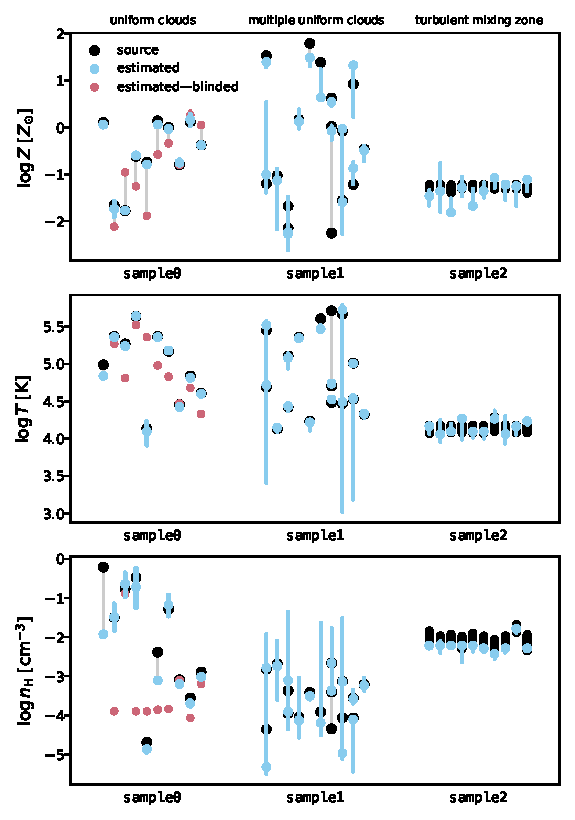
\includegraphics[width=\columnwidth]{figures/summary.pdf}
    \caption{
    The source properties (black) used to produce the synthetic absorption systems
    compared to the best estimates from parameter estimation across all three of our samples.
    Red are the parameter estimates from fully-blind modeling,
    and blue are the final parameter estimates.
    The lines span the 16th to 84th percentiles of the parameter-estimation posteriors or source data when available.
    The samples range from uniform clouds to a turbulent mixing zone.
    For the turbulent mixing zone the \ion{H}{I}-weighted average of the source data is shown.
    The parameter-estimation best estimates and the source data typically agree to $\lesssim$ ( 0.5 dex in $Z$, 0.3 dex in $T$, 1 dex in $n_{\rm H}$),
    excluding the blinded \texttt{sample0} estimates (\S\ref{s: results -- sample0}).
    }
    \label{f: summary}
\end{figure}

% \begin{figure}
%     \centering
%     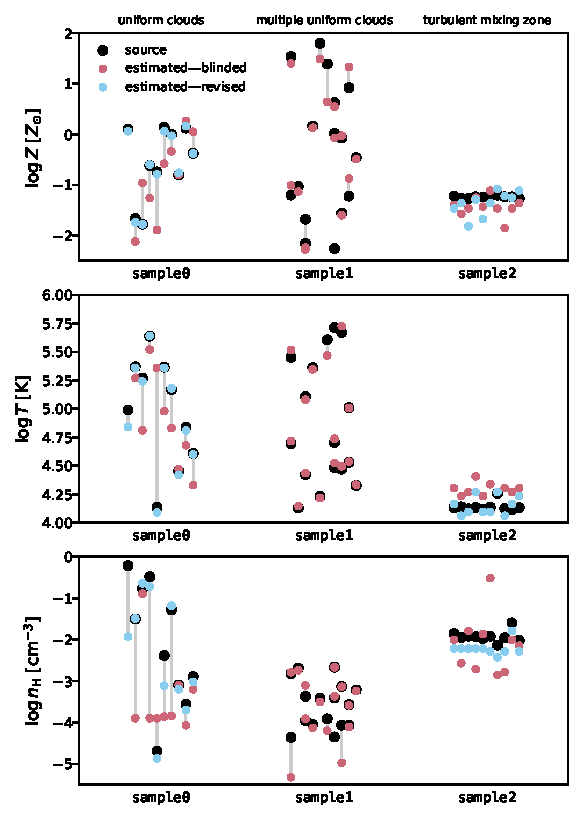
\includegraphics[width=\columnwidth]{figures/averages.pdf}
%     \caption{
%     The source properties (black) used to produce the synthetic absorption systems
%     compared to the best estimates from parameter estimation across all three of our samples.
%     Red are the parameter estimates from fully-blind modeling,
%     and blue are the parameter estimates following any revision.
%     The samples range from uniform clouds to a turbulent mixing zone.
%     For the turbulent mixing zone the \ion{H}{I}-weighted average of the source data is shown.
%     The parameter-estimation best estimates and the source data typically agree to $\lesssim$ ( 0.5 dex in $Z$, 0.3 dex in $T$, 1 dex in $n_{\rm H}$),
%     excluding the blinded \texttt{sample0} estimates (\S\ref{s: results -- sample0}).
%     }
%     \label{f: summary--average}
% \end{figure}

% \begin{figure}
%     \centering
%     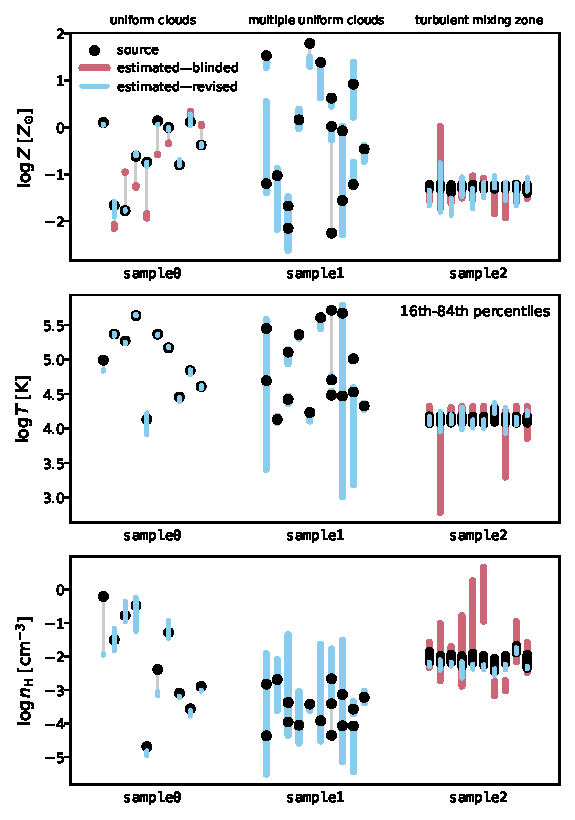
\includegraphics[width=\columnwidth]{figures/percentiles.pdf}
%     \caption{
%     Same as Figure~\ref{f: summary--average},
%     but with lines spanning the 16th to 84th percentiles of the parameter-estimation posteriors or source data when available.
%     Posteriors that overlap the source data suggest that the parameter estimation is sufficiently conservative to capture the range of possible properties for the absorbing gas.
%     For \texttt{sample1} and \texttt{sample2} the posteriors typically overlap with the source data,
%     with the exception of the \texttt{sample2}-revised $n_{\rm H}$ posteriors.
%     For \texttt{sample0} the parameter estimation methodology had to be adapted to work with a set of provided column densities instead of full spectra,
%     limiting the extent and interpretation of the provided errors.
%     }
%     \label{f: summary--widths}
% \end{figure}

% Summary of averages
We discuss the per-sample results in the following subsections,
while Figure~\ref{f: summary} summarizes some of the key results.
The overlap of points in Figure~\ref{f: summary} reflects the agreement between the parameter-estimation best estimates and the average source properties.
For \texttt{sample0} and \texttt{sample1} we show one value per cloud for both the source and parameter estimations.
For \texttt{sample2} the source data is a distribution of clouds, and therefore we show the \ion{H}{I}-weighted average of the source distributions compared to the \ion{H}{I}-weighted maximum likelihood estimates from parameter estimation.
The strongest disagreements are for the blinded estimates in \texttt{sample0} (\S\ref{s: results -- sample0}), although the densities are systematically underpredicted for \texttt{sample2}.

% Summary of widths
The lines in Figure~\ref{f: summary} summarize the extent to which the source data lies within the expected range of values from parameter estimation.
In \texttt{sample0} and \texttt{sample1} the source data are discrete values per cloud,
and correspondingly we show one posterior per cloud.
In \texttt{sample2} the black lines span the 16th to 84th percentiles of the \ion{H}{I}-weighted source distributions,
and the colored lines span the 16th to 84th percentiles of the combined \ion{H}{I}-weighted posteriors (the parameter estimation in \texttt{sample2} estimates a number of clouds, and the posteriors from each individual cloud are joined into a combined posterior).

\subsection{Column densities of uniform clouds --- \texttt{sample0}}
\label{s: results -- sample0}

% Trying removing this figure and just referring to the left panel of the preceding figures.
\begin{figure}
    \centering
    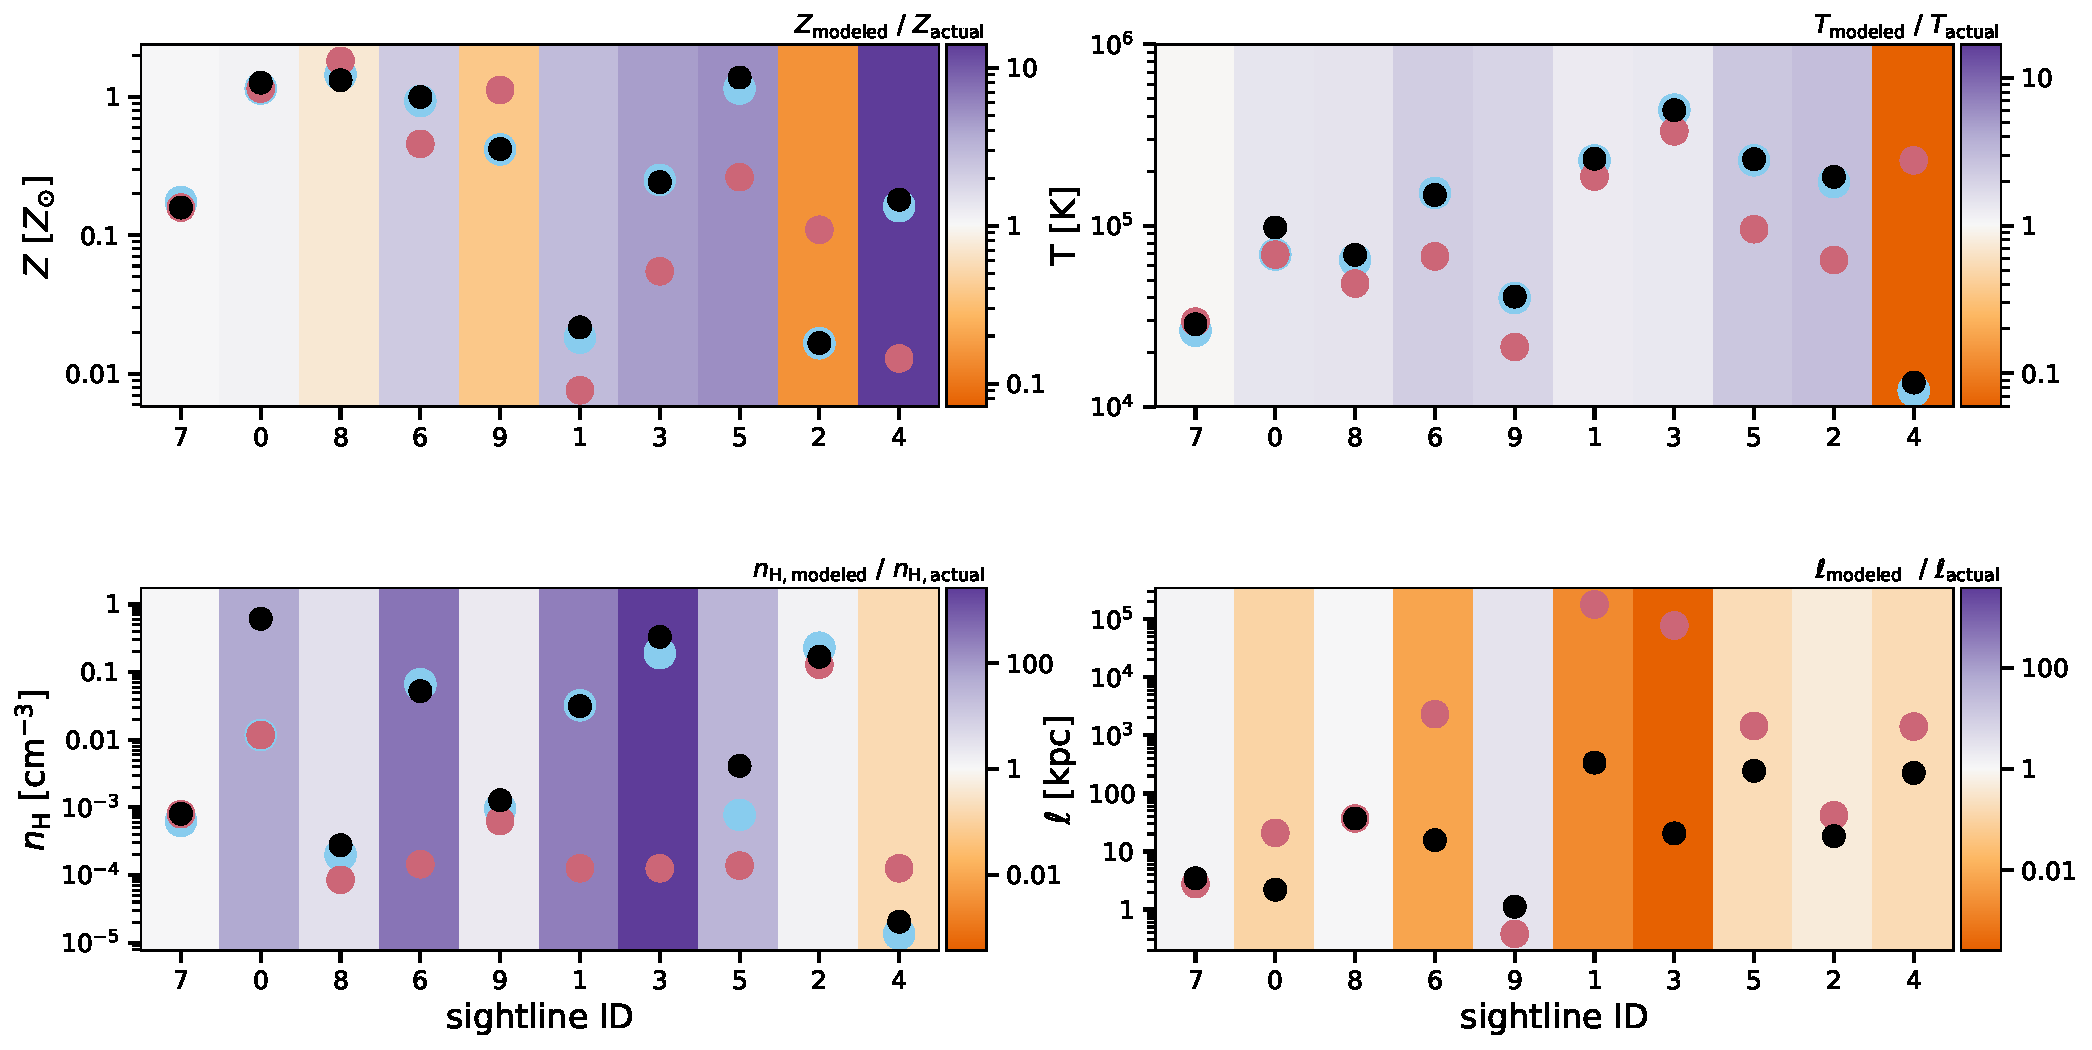
\includegraphics[width=\columnwidth]{figures/sample0/comparison.pdf}
    \caption{
    Comparison between estimated and source properties of highly-idealized absorption systems (\texttt{sample0}).
        Black, red, and blue points show the source, blinded, and revised values respectively for each property.
    Sightlines are ordered from left to right according to agreement between the blinded modeled metallicity and the source metallicity.
   The blinded parameter estimates assumed thermal equilibrium,
   while the revised estimates removed this assumption and had excellent recovery of the source properties.
   The revised recovery of the source properties is despite many of the source quantities having unusual combinations of density and temperature (Figure~\ref{f: idealized explanation}).
    }
    \label{f: idealized}
\end{figure}

\begin{figure}
    \centering
    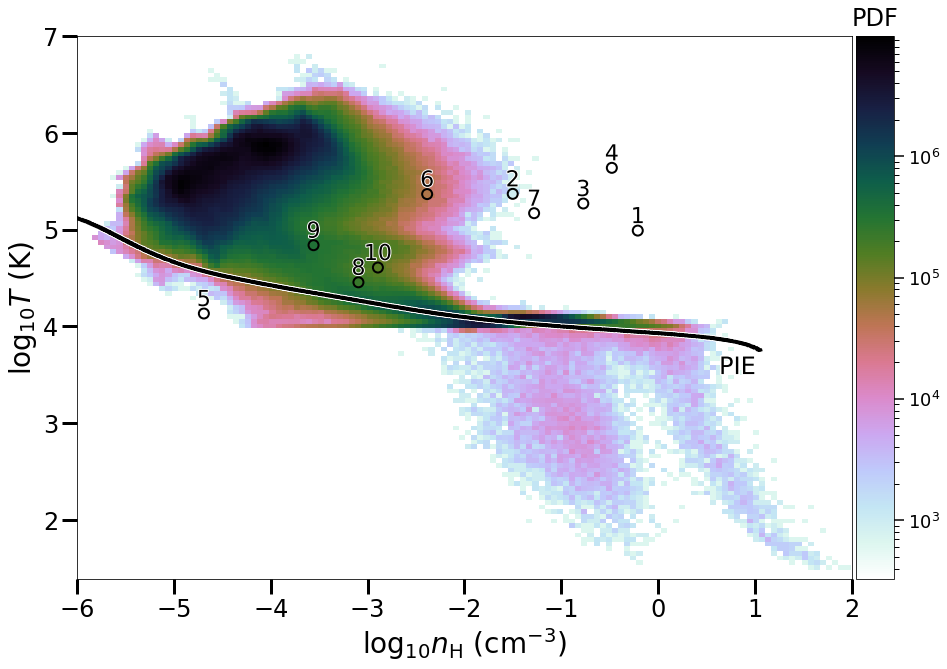
\includegraphics[width=\columnwidth]{figures/sample0/phase_space.png}
    \caption{
    Comparison between estimated and actual properties of \texttt{sample0} in the context of the temperature-vs-density distribution of CGM gas in a FIRE-2 cosmological simulation (black background distribution; scales with logarithmic PDF and includes satellite ISM).
    The solid black line shows the range of temperatures and densities where gas is in thermal equilibrium via photoheating.
    If thermal equilibrium is assumed during parameter estimation then when the assumption is inaccurate the estimated metallicity tends to be inaccurate.
    However, in the simulation there is a large population of CGM gas that is in approximate thermal equilibrium.
    }
    \label{f: idealized explanation}
\end{figure}

% Intro
Figure~\ref{f: idealized} shows the results of parameter estimation for \texttt{sample0}.
The blinded estimates (red)  are the observers' first estimates given the data and no additional information.
After the observers compared the blinded estimates to the revealed source properties they made adjustments to their methodology and performed parameter estimation again.
The results are the revised estimates (blue).
For \texttt{sample0} the primary revision to methodology was removing the assumption of thermal equilibrium.
The same procedure was also applied to all sightlines, instead of adapting the methodology to the sightline.

% A tale of priors
The discrepancies between the estimated properties and the source properties are driven by the assumptions made by both observers and theorists.
Theorists created \texttt{sample0} by randomly sampling properties from a uniform distribution for each property, assuming for simplicity the properties are independent.
Subsequently, while in isolation each property was characteristic of CGM gas, in combination the properties described gas atypical for the CGM.
This is seen in Figure~\ref{f: idealized explanation}, which compares the temperatures and densities of the source clouds to temperatures and densities typical for the CGM in a cosmological simulation (this particular data is part of the FIRE-2 public data release,~\citealt{wetzel2022Public}).
On the other hand, the observers modeled \texttt{sample0} with assumptions informed by current knowledge of the CGM.
For example, the observers tested if the column densities were consistent with thermal equilibrium driven by photo-ionization equilibrium, in which case the estimated temperature is a calculated from the estimated metallicity and density parameters.
Under these assumptions the observers found reasonable fits to the provided column densities for sightlines \texttt{06} through \texttt{10}.
Observers found reasonable observed-column-density fits for three of the other sightlines after fixing the density to an assumed $n_{\rm H} = 10^{-3.9}$ cm$^{-3}$ and assuming collisional ionization.
In this case, the temperature can be determined, but the metallicity also depends on the density,
which was not actually close to the assumed value.

In the revised modeling observers removed any assumptions of thermal equilibrium, and found much better agreement with the source properties.
Even still, in four of the ten sightlines (\textsc{01}, \textsc{02}, \textsc{06}, \textsc{07}) the best fit parameters had total \ion{H} column densities outside the parameter space \textsc{cloudy} is designed to handle, which required observers to identify and scale solutions with the same ion densities but less total mass.

To summarize, the \texttt{sample0} models were not realistic based on the parts of parameter space occupied by the synthetic data and the initial parameter estimation assumptions were too rigid.
The lesson learned is that there will be places in the real universe where heating and cooling do not balance, and the solution that observers obtain may not be unique.
This is particularly true for higher ionization gas (at $T \gtrsim 10^{5}$ K and/or $n_{\rm H} \lesssim 10^{-2}$ cm$^{-3}$),
but the effects may also be stronger because only ion column densities were provided (as opposed to full spectra).

\subsection{Spectra of multi-cloud systems --- \texttt{sample1}}
\label{s: results -- sample1}

\begin{figure*}
    \centering
    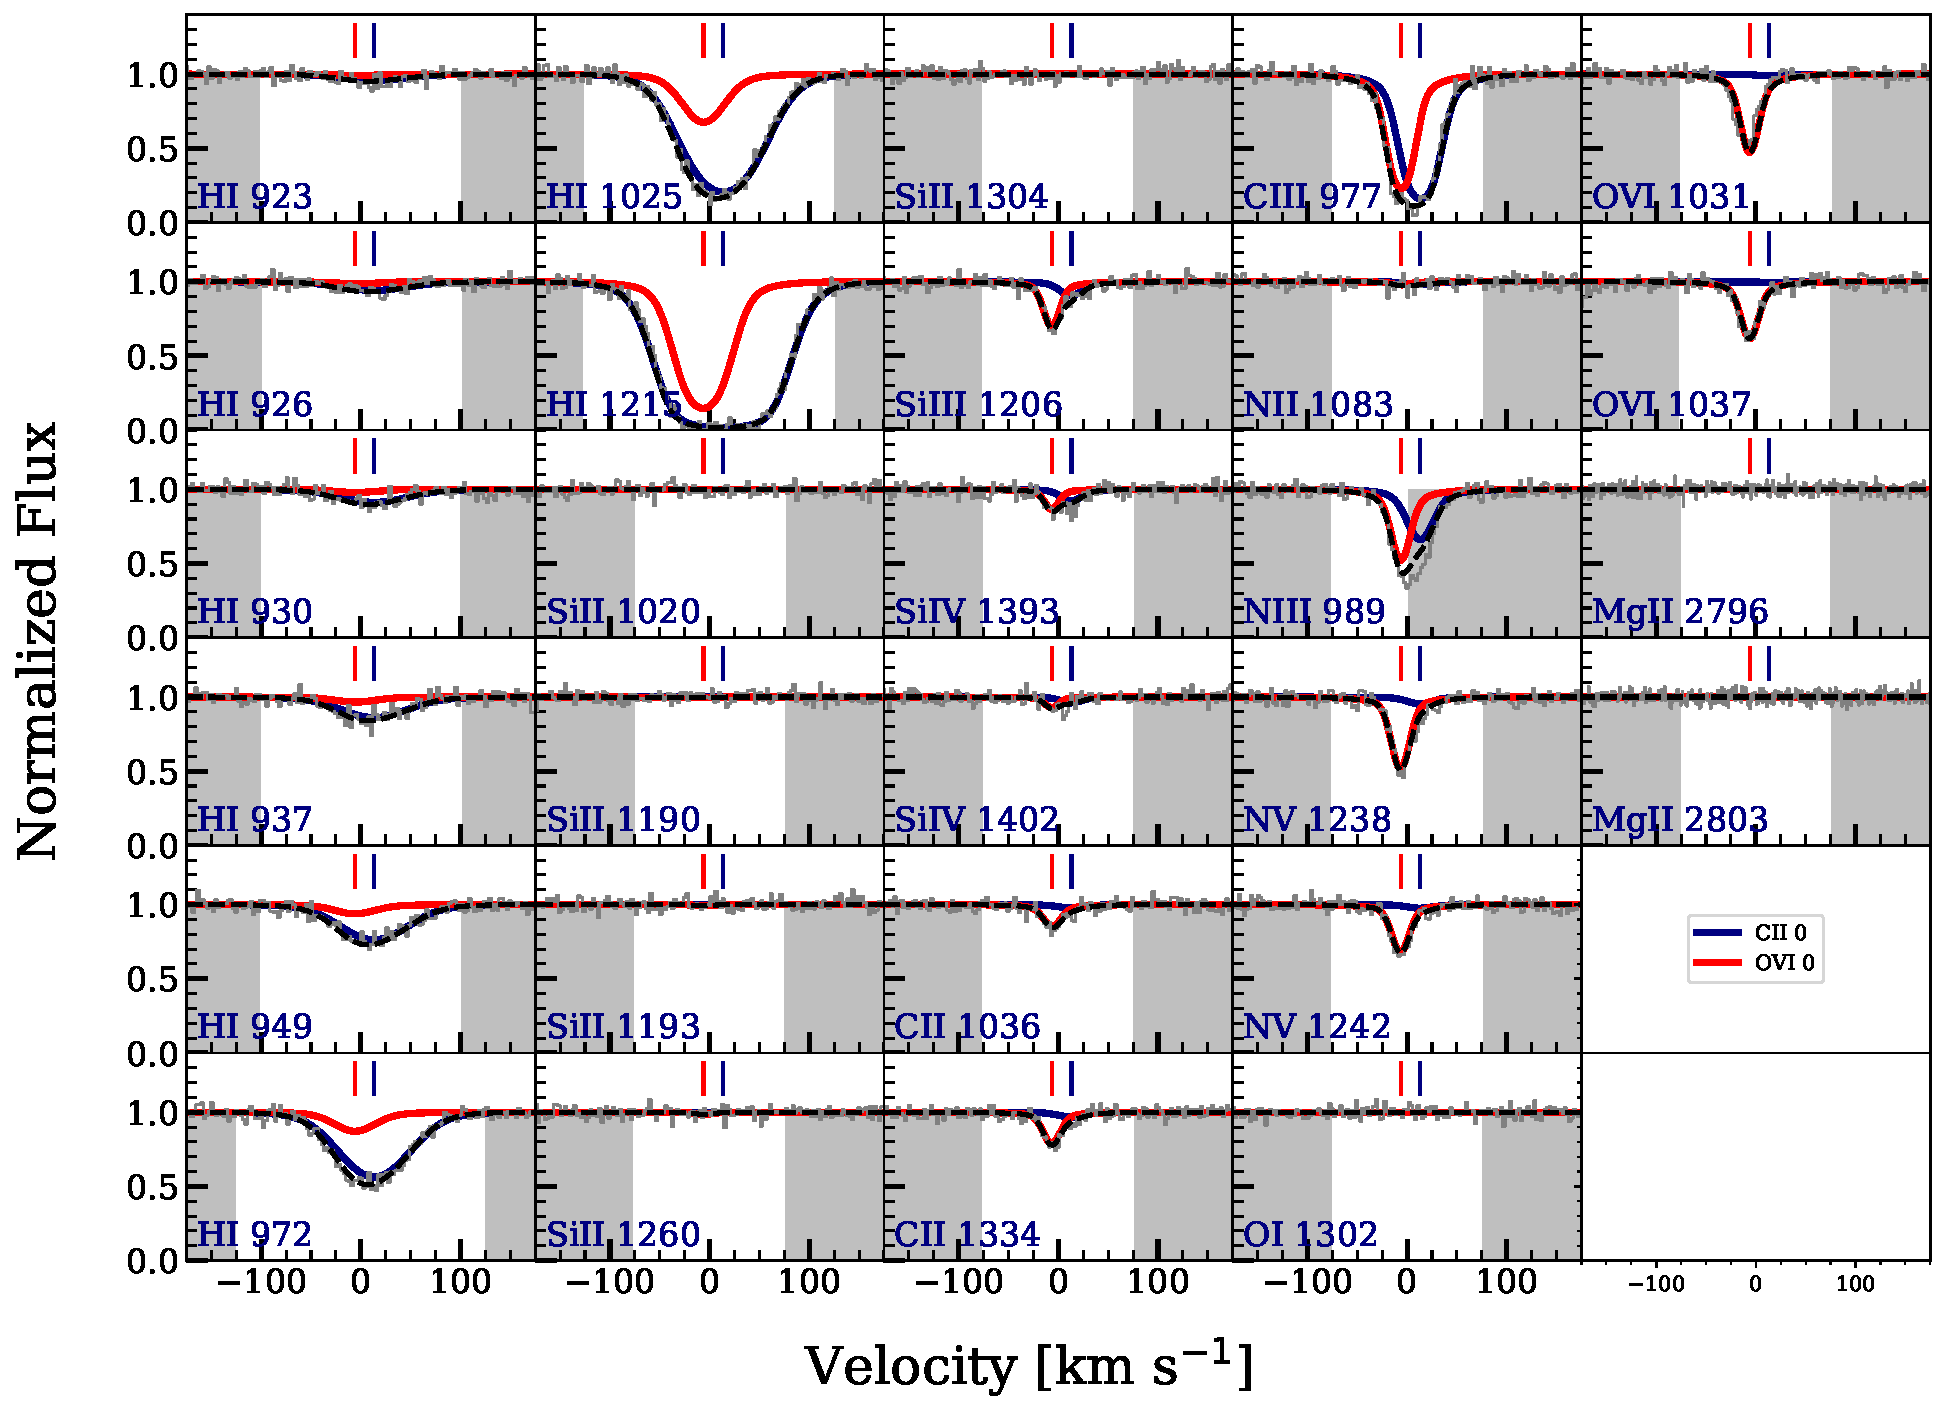
\includegraphics[width=\textwidth]{figures/sample1/Models_076.pdf}
    \caption{
    The source spectrum (grey steps) and the parameter-estimation best-fit spectrum (dashed black) for sightline 076 in \texttt{sample1}.
    The data are best fit by a two-cloud model, and the Voigt profiles of the individual components are shown in dark blue and red. 
    The dark blue curve traces the phase that produces the bulk of the \ion{H}{I} absorption, and the red curve traces the phase that produces \ion{O}{VI} absorption.
    The spectrum wavelength was converted to line-of-sight velocity in this image,
    and the velocity of each component is indicated by a vertical dash.
    The grey bands show the portion of the spectrum with no influence on parameter estimation.
    }
    \label{f: sample1 spectrum}
\end{figure*}

\begin{figure}
    \centering
    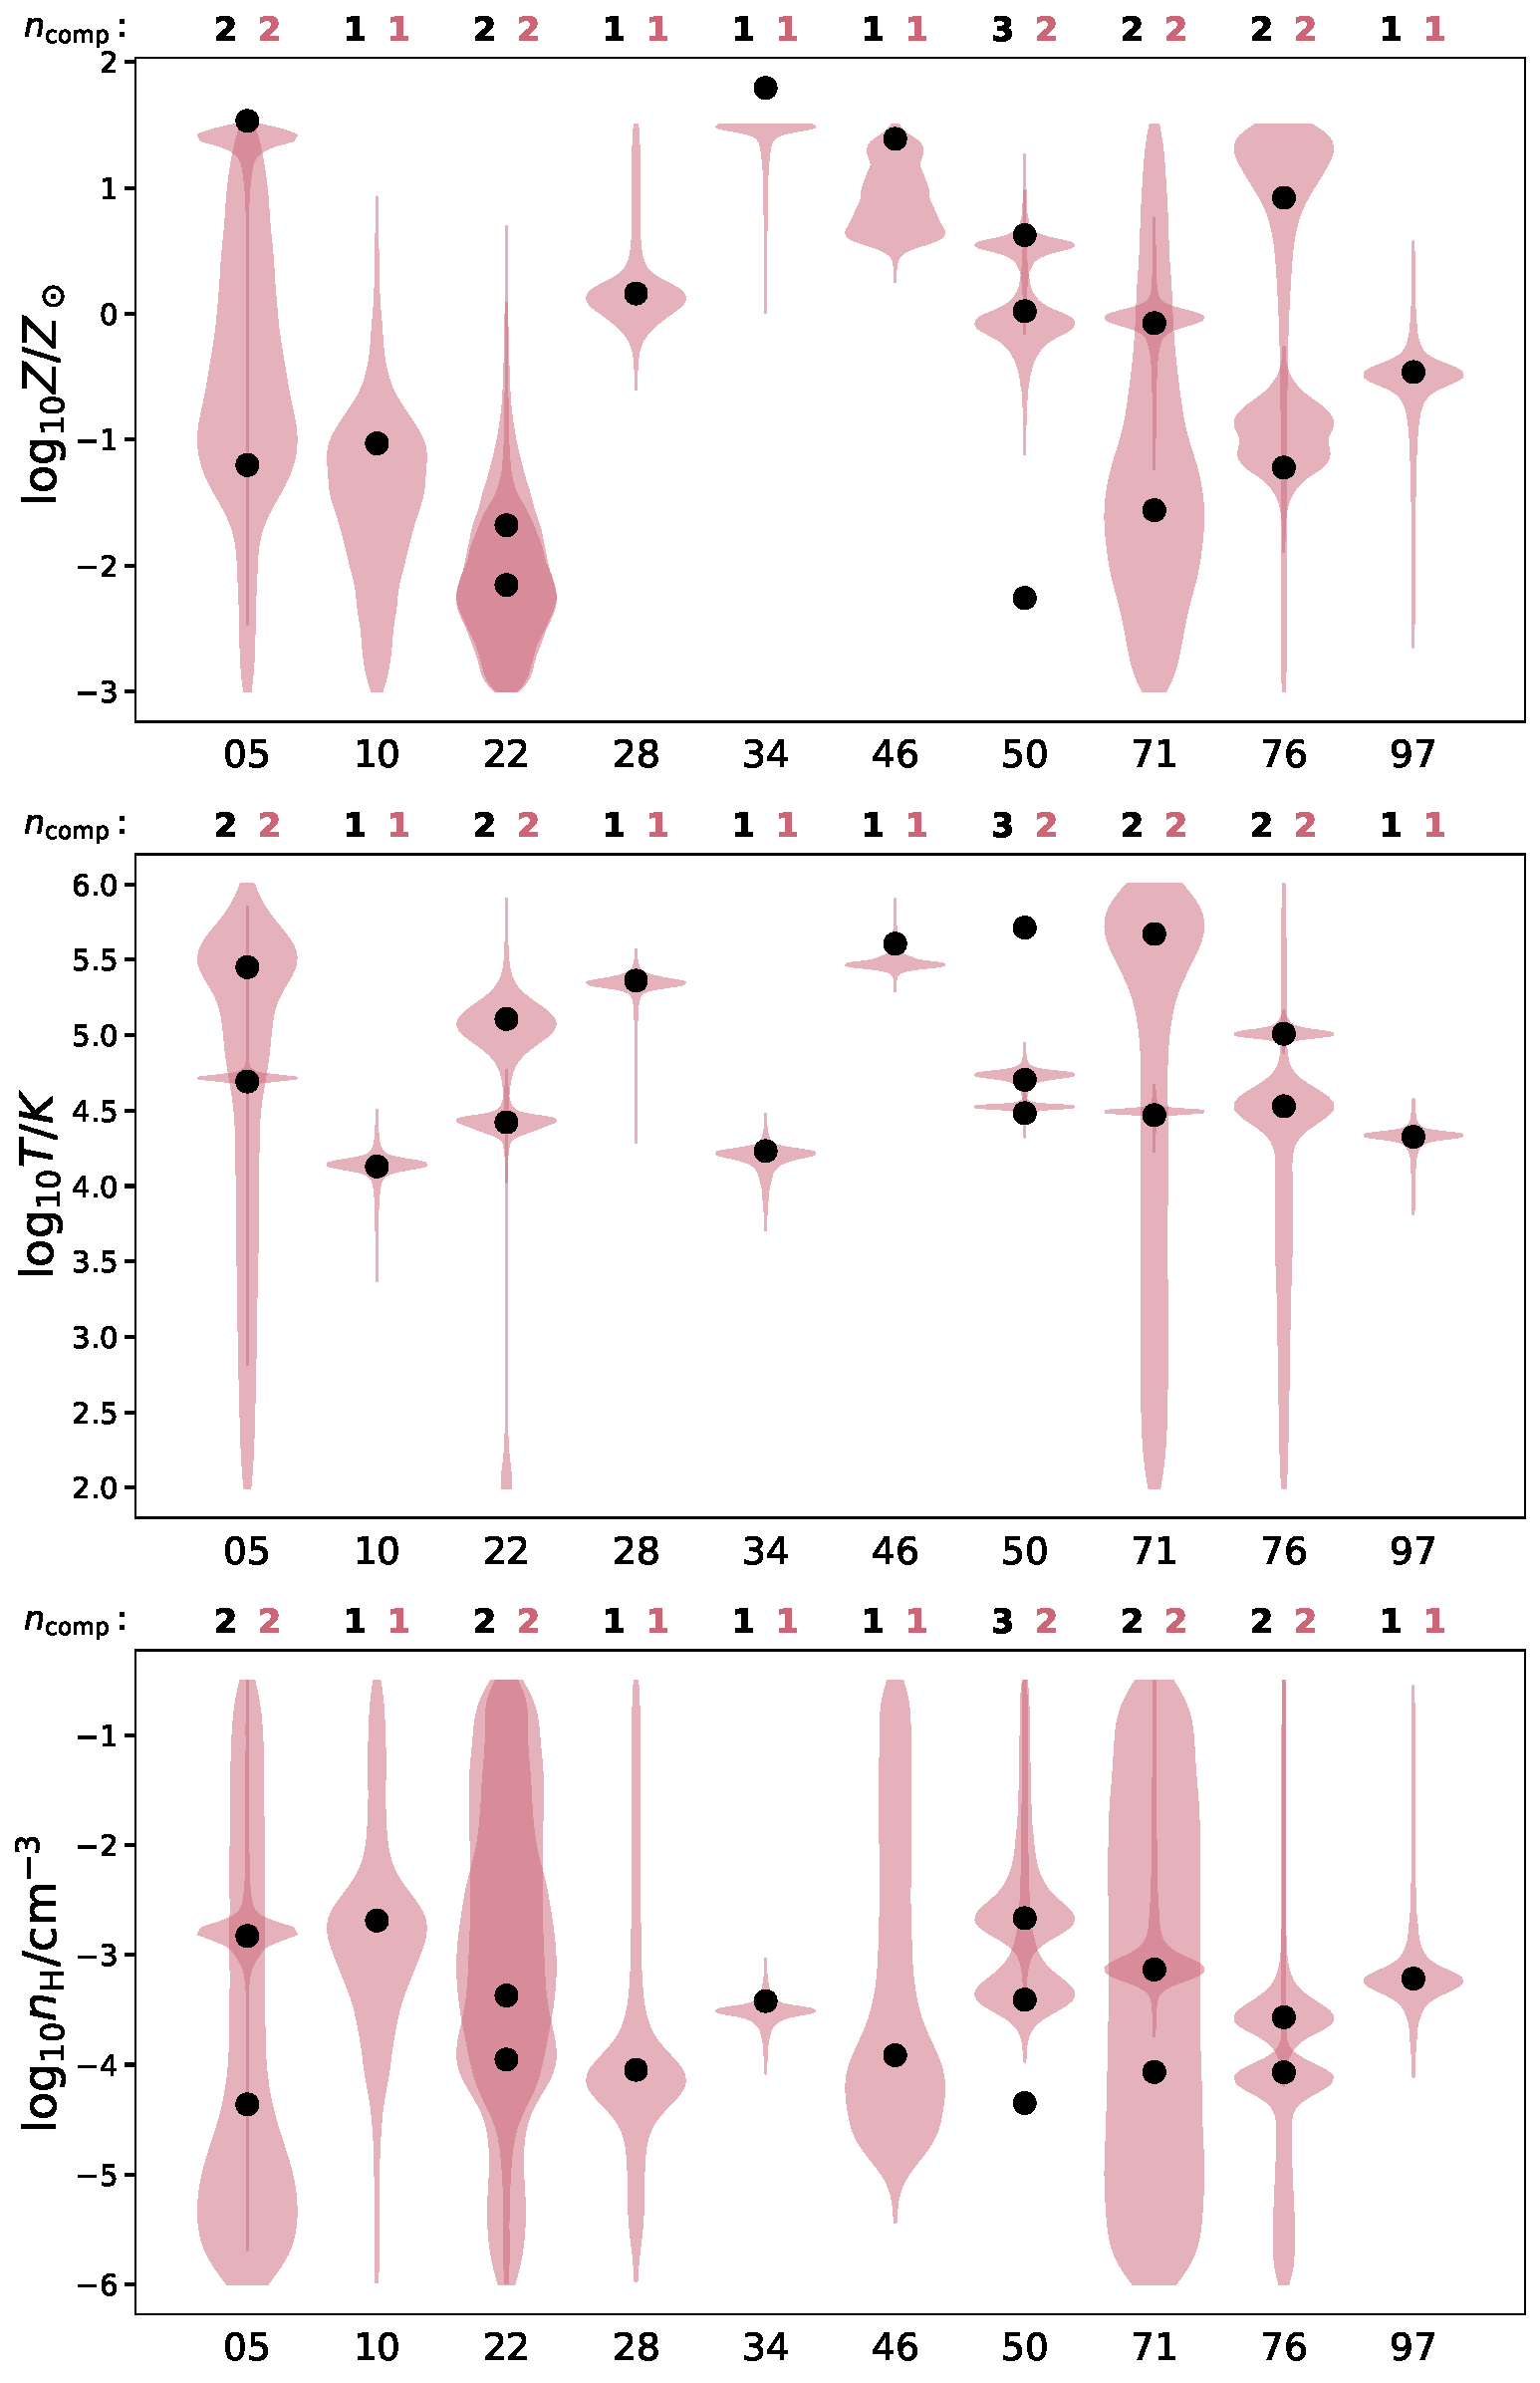
\includegraphics[width=\columnwidth]{figures/sample1/comparison.pdf}
    \caption{
    Synthetic data properties for multiple uniform clouds (\texttt{sample1}, black) compared to posteriors from parameter estimation (red).
    The wider the ``violin'' plots, the larger the value of the posterior at that parameter (e.g. temperature) value.
    The numbers above each sightline indicate the number of source clouds and the estimated number of clouds.
    The maximum likelihood estimates (the peak values of the posteriors) typically align with the source parameters.
    }
    \label{f: sample1 violin}
\end{figure}

% Spectra
In Figure~\ref{f: sample1 spectrum} we show an example spectrum provided to observers as part of \texttt{sample1}, and the Voigt profiles from the parameter-estimation best fits.
The grey bands indicate areas that are masked and do not contribute to parameter estimation because there is a blend known to contaminate the spectrum or because there is no detected absorption in the region.
For \texttt{sample1} the parameter-estimation best fit was selected from models with varying numbers of clouds. In this sightline, the data is best fit by two clouds, one with significant low-ion absorption (e.g. \ion{C}{III})  and one with significant high-ion absorption (e.g. \ion{O}{VI}).
\atsameer{How do you decide on your component names? It was pointed out to me that the \ion{O}{VI} component in Figure~\ref{f: sample1 spectrum} actually dominates the \ion{C}{II} absorption.}
In \texttt{sample1} the observers did not perform a revised parameter estimation because the blinded parameter estimates agreed well with the source data, in part because thermal equilibrium was not assumed.

% Comparison to data
Figure~\ref{f: sample1 violin} compares the posteriors from the parameter estimation to the properties of the source clouds.
Posterior probability distributions, or posteriors for short, describe the predicted probability of the source properties having a given value.
The posteriors are displayed via a violin plot,
where the width of the vertical distribution at a given value scales with the posterior probability distribution at that value.
Violin plots are equivalent to histograms rotated 90$^\circ$ and reflected to be symmetric.
In most cases the source properties reside well inside the posteriors, i.e. the posteriors are typically sufficiently broad.
As with the blind modeling for \texttt{sample0} some actual values lie outside the assumed range of possible values: 
some source clouds have $Z > 10^{1.5} Z_\odot$, while the parameters were estimated assuming $Z$ spans $\log_{10} Z/Z_\odot = [-3, 1.5]$ (where $\log_{10} Z/Z_\odot = 1.5$ is the default metallicity range for Cloudy).
However, the source $Z$ are within $< 0.5$ dex of the highest estimated metallicity, significantly less discrepant than blind modeling for \texttt{sample0}.

% Wide posteriors.
The widest posteriors in \texttt{sample1} are often associated with a hotter phase tracing the OVI for a few reasons.
First, the cooling of such a gas phase resembles that of collisional time-dependent gas cooling with no external radiation, and hence is independent of density.
\atsameer{I'm trying to understand this cooling better. Why is cooling not going as $n^2$? Do you have a reference I can look at to read up on this?}
Second, following the lessons learnt from \texttt{sample0}, the observers relaxed the priors such that the lowest temperature could be $10^2$ K, while the source data has a lower bound of $10^4$.
\atsameer{Why is the hottest gas also the one with posteriors reaching down to the lowest limits? If the issue is that it's hot, how come the posteriors aren't limited to $T \gtrsim 10^4.5$ K?}
A potential second mode is being reflected in the parameter estimates, which may not be realistic. 
Additional potential contributing factors to the wide posteriors include the absence of \ion{C}{IV} lines in the provided spectra (\ion{C}{IV} 1548, 1550 probe intermediate temperatures and are not covered by COS G130M or G160M at $z=0.25$), 
and the stated error in the provided spectra.

% Number of components
The modeling identifies the correct number of components in 9 of 10 sightlines.
The exception is sightline 050, which has a hot, low-density, low-metallicity absorber that produces little absorption in the ions provided to the observers.

\subsection{Spectra of high-resolution turbulent mixing --- \texttt{sample2}}
\label{s: results -- sample2}

\begin{figure*}
    \centering
    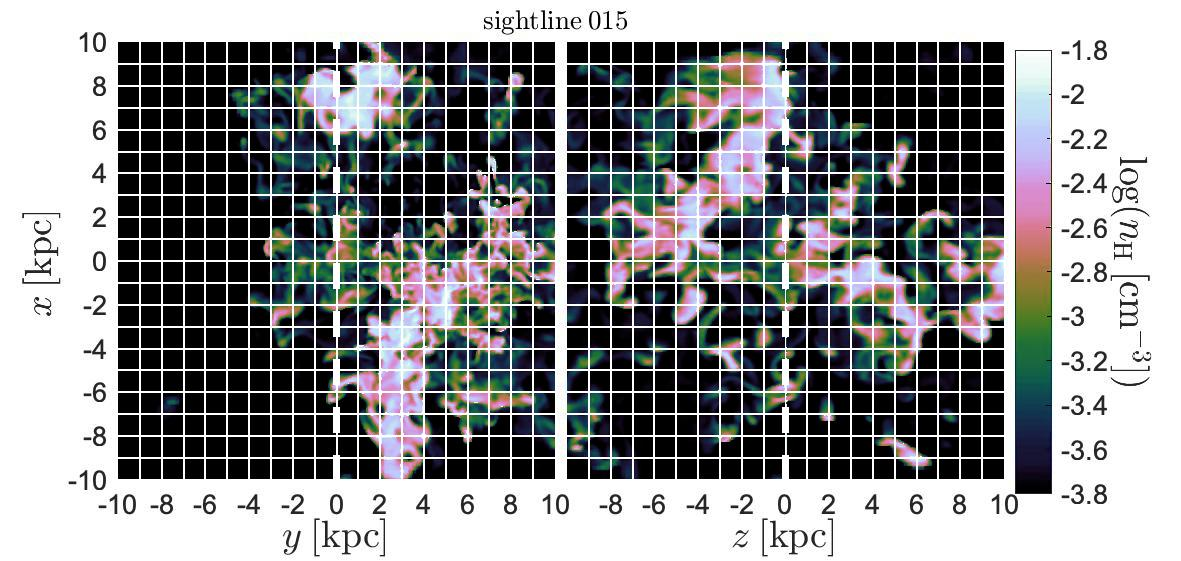
\includegraphics[width=0.49\textwidth]{figures/sample2/projections/density_projection_maps_SL_15.jpg}
    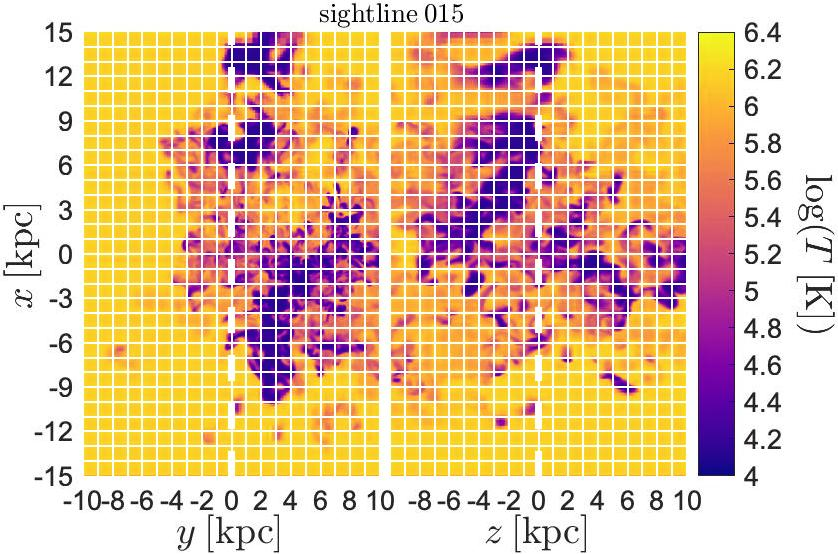
\includegraphics[width=0.49\textwidth]{figures/sample2/projections/temperature_projection_maps_SL_15.jpg} \\
    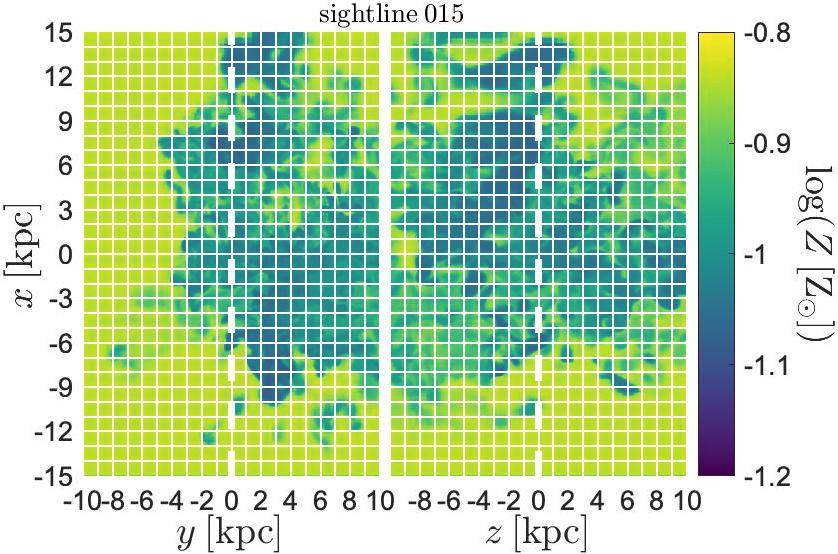
\includegraphics[width=0.49\textwidth]{figures/sample2/projections/metallicity_projection_maps_SL_15.jpg}
    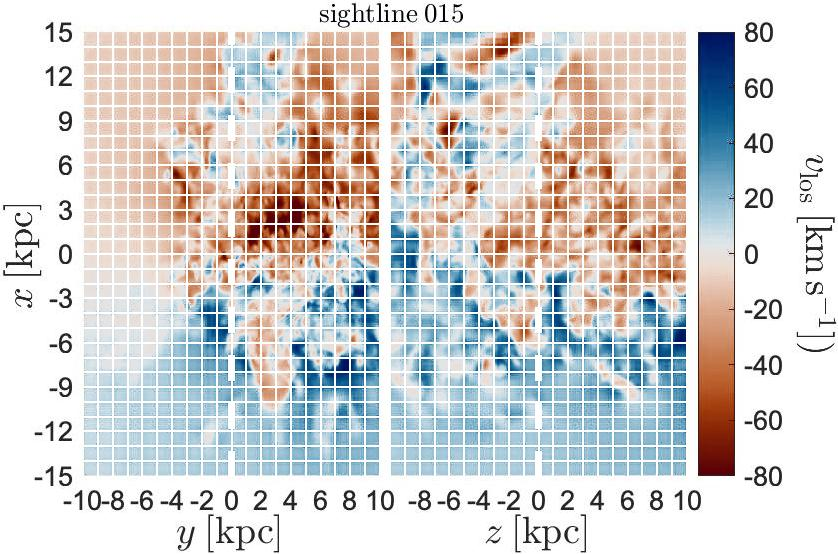
\includegraphics[width=0.49\textwidth]{figures/sample2/projections/velocity_projection_maps_SL_15.jpg}
    \caption{
    Density, temperature, metallicity, and line-of-sight velocity in a slice of the simulation used to generate \texttt{sample2}~\citep{mandelker2020Instability}.
    The dashed white line shows the location of one of the sightlines (sightline 15) forward-modeled to produce mock spectra.
    The simulation includes a turbulent mixing zone, and shows highly complex cloud structure.
    A grid with 1 kpc spacing is overlaid in white to help the viewer gauge cloud size.
    }
    \label{f: sample2 ray 15}
\end{figure*}

\begin{figure*}
    \centering
    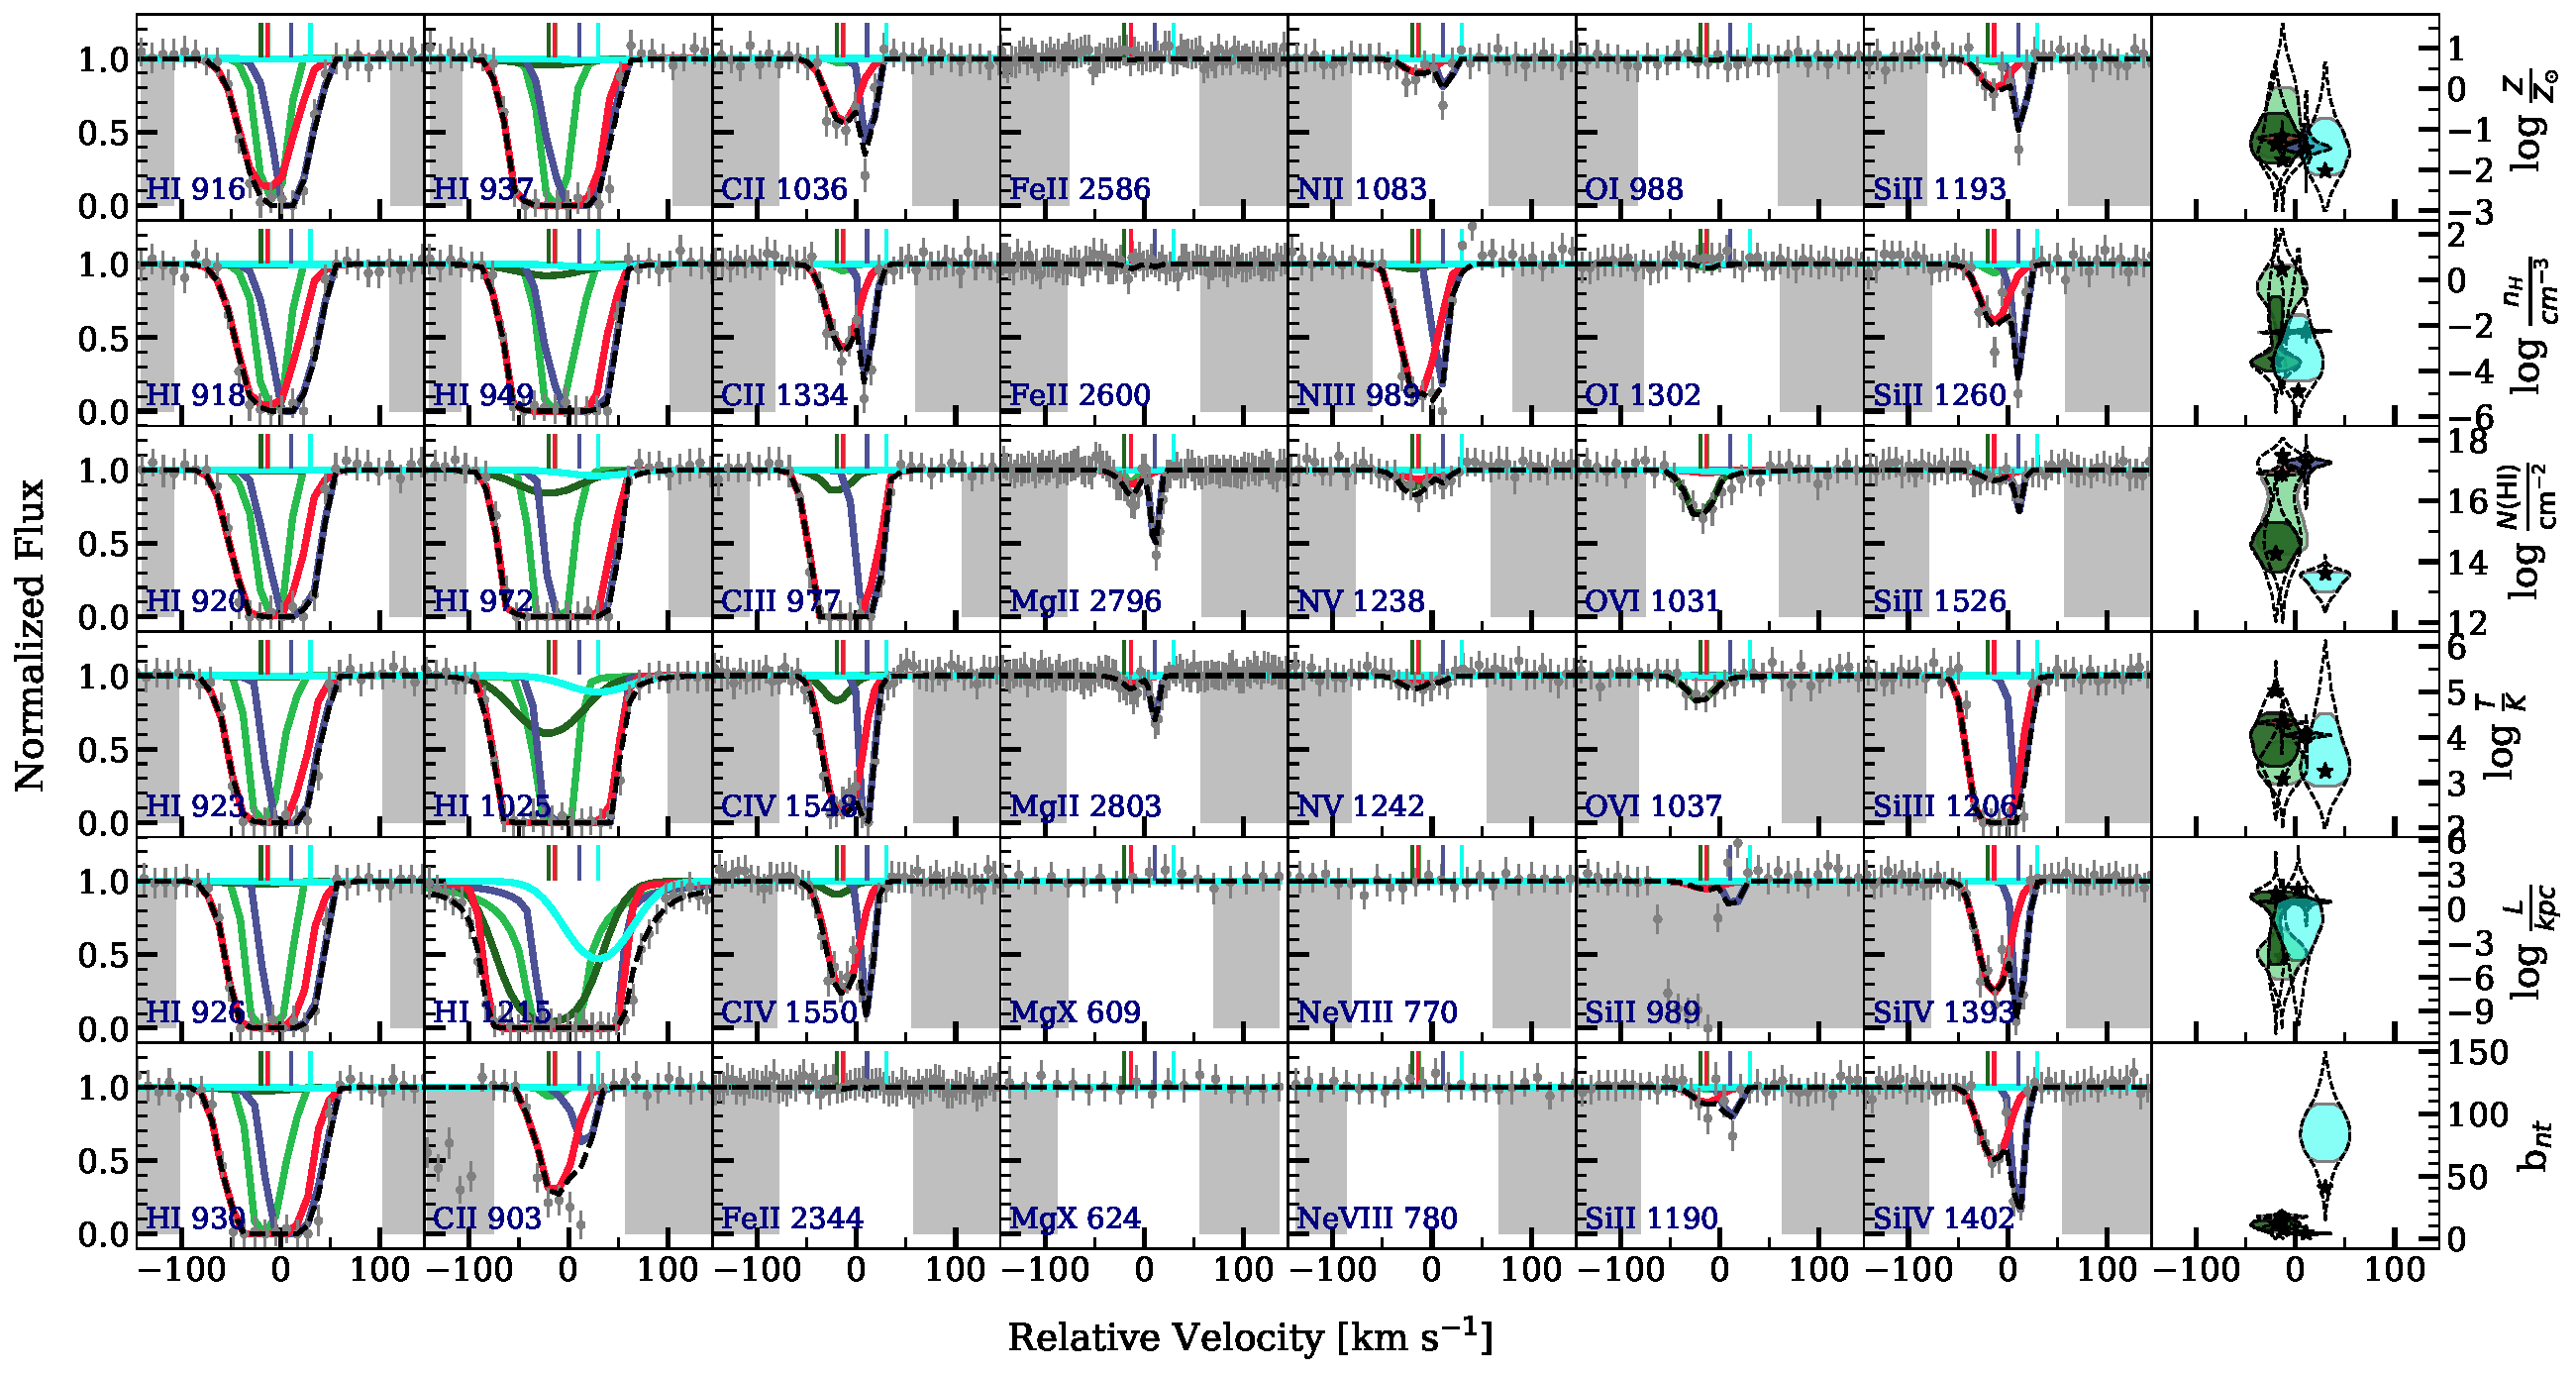
\includegraphics[width=\textwidth]{figures/sample2/best_fits/0015.pdf}
    \caption{
    Mock spectra for the sightline shown in Figure~\ref{f: sample2 ray 15},
    best fit absorption profiles found by observers,
    and the parameters of the best fits.
    The absorption along this sightline is best fit by five components.
    \atsameer{Are the stars MLEs? If so, why are some not at the distribution peak? Thanks for your answer, I've added further questions in the response.}
    }
    \label{f: sample2 spectrum 15}
    \end{figure*}

\begin{figure*}
    \centering
    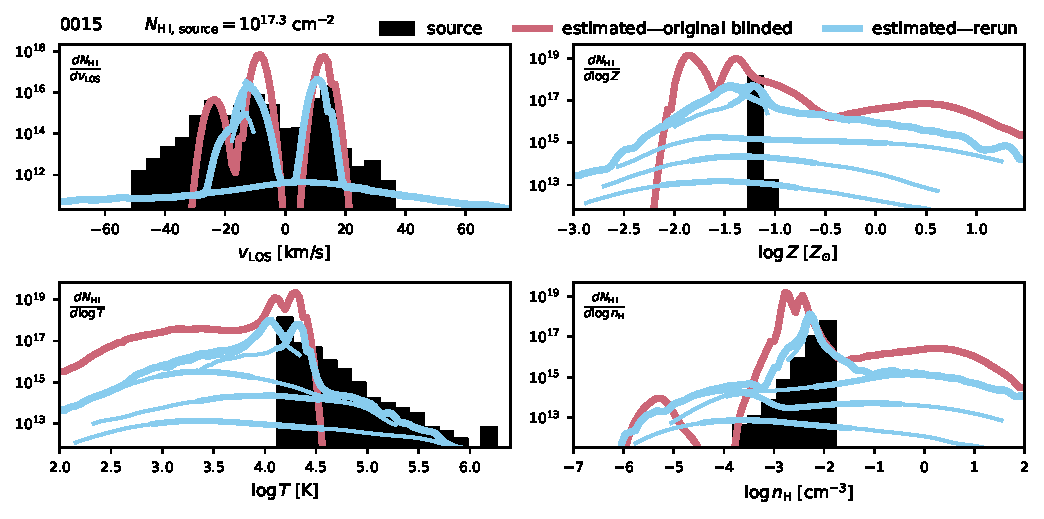
\includegraphics[width=\textwidth]{figures/sample2/high-z/sightline_0015.pdf}
    \caption{
    Estimated and source properties of gas along the sightline shown in Figures~\ref{f: sample2 ray 15} and \ref{f: sample2 spectrum 15}.
    Black shows the source properties used to produce the mock spectra.
    Blue show the posteriors from the parameter estimation. 
    The combined posteriors are indicated by thick lines (except for $v_{\rm LOS}$, where the posteriors are narrow enough to use vertical bars).
    We also show the posteriors for individual clouds as blue lines outlined in thick (thin) black, for the regions enclosing 68\% (99.7\%) of the posterior for a given cloud.
    }
    \label{f: sample2 15}
\end{figure*}

\begin{figure}
    \centering
    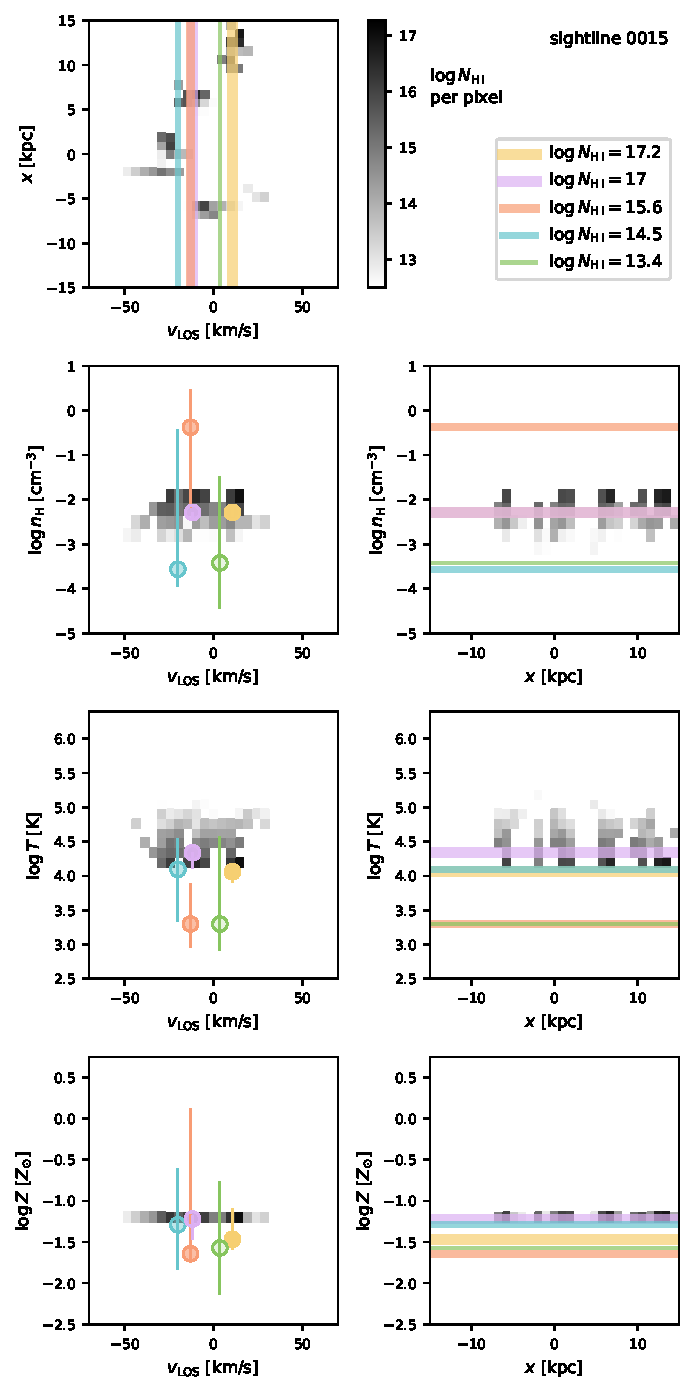
\includegraphics[width=\columnwidth]{figures/sample2/high-z/component_structure_0015.pdf}
    \caption{
    Physical- and velocity-space cloud structure for the sightline shown in Figures~\ref{f: sample2 ray 15}, \ref{f: sample2 spectrum 15}, and \ref{f: sample2 15}.
    The top left panel shows the relationship between position along the line of sight ($x$) and the line-of-sight velocity of the gas.
    Source properties are plotted with black 2D histograms,
    while the colors correspond to estimated components.
    The estimated components accurately describe the gas responsible for the vast majority of the absorption.
    However, gas aligned in velocity but physically separated can introduce confusion to the interpretation,
    and it is challenging to constrain the shape of the cloud property distributions.
    }
    \label{f: sample2 structure 15}
\end{figure}

\begin{figure*}
    \centering
    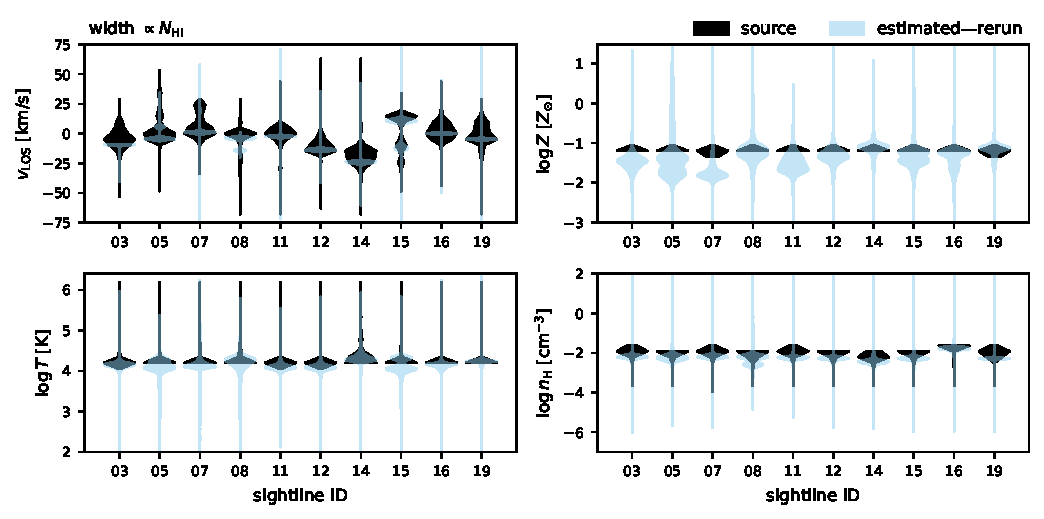
\includegraphics[width=\textwidth]{figures/sample2/violin_rerun.pdf}
    \caption{
    The distributions of $v_{\rm LOS}$, $Z$, $T$ and $n_{\rm H}$ for the synthetic source data (black) compared to the full posteriors from parameter estimation (revised only; blinded in Appendix~\ref{a: sample2 blinded}).
    The width of the violin plots scales with $N_{\ion{H}{I}}$.
    The parameter estimation accurately describes the properties of the gas responsible for the majority of the absorption.
    }
    \label{f: sample2 violin}
\end{figure*}

\begin{figure*}
    \centering
    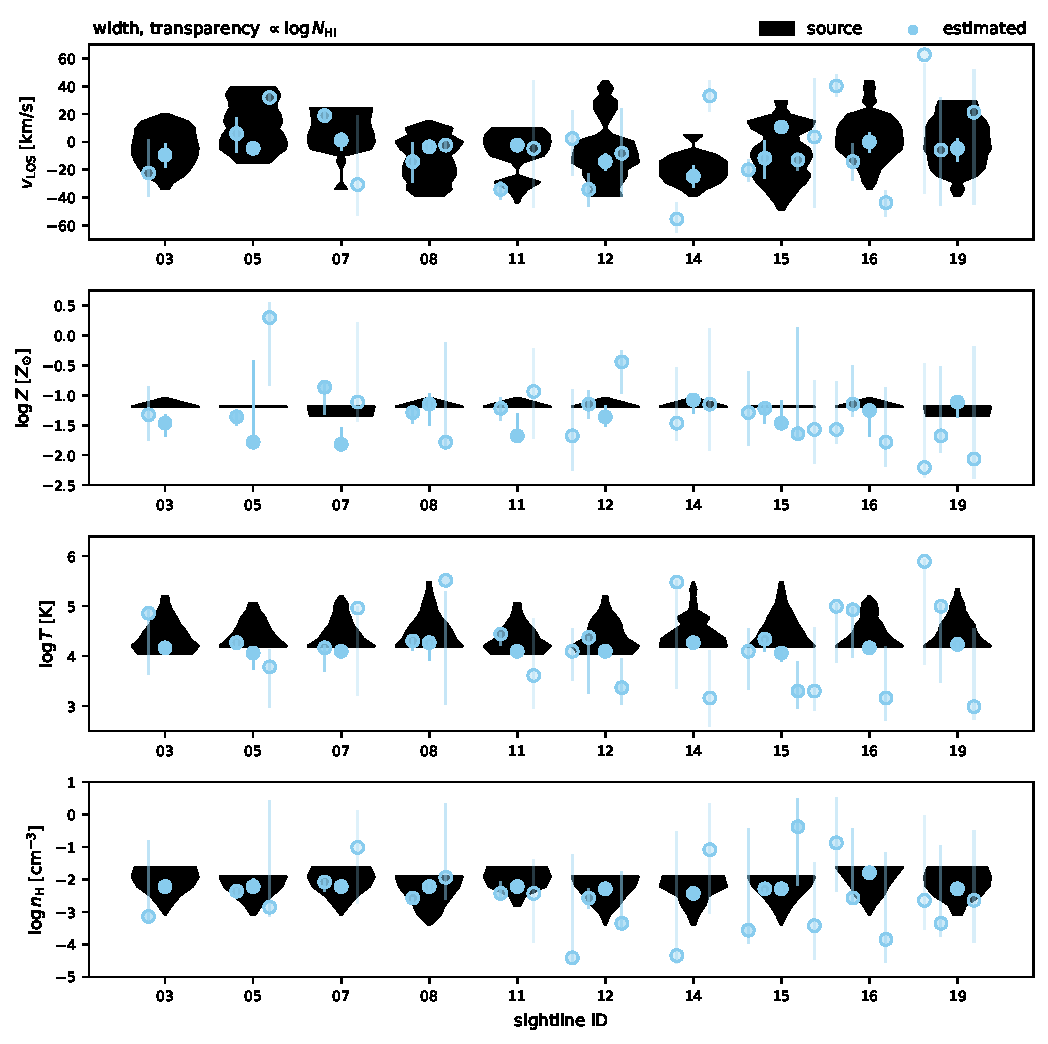
\includegraphics[width=\textwidth]{figures/sample2/violin_vs_components_rerun.pdf}
    \caption{
    The distributions of $v_{\rm LOS}$, $Z$, $T$ and $n_{\rm H}$ for the synthetic source data (black) compared to the best estimates for individual components comprising the parameter estimation.
    Each point is the maximum-likelihood estimate (MLE) of an individual component,
    and the associated bars enclose the 16th to 84th percentiles of the posterior.
    The width of the violin plots and the opacity of the points are scaled \textit{logarithmically} with $N_{\ion{H}{I}}$,
    such that if the parameter estimation perfectly agreed with the data all visible MLE points would lie within the source data violins.
    The MLE of the strongest-$N_{\ion{H}{I}}$ component typically describes the parameters of most of the absorbing gas---the largest errors are in $Z$ and at a $\lesssim 1$ dex level.
    The lower-$N_{\ion{H}{I}}$ components trace some features of the underlying distribution,
    but arguably the lower-$N_{\ion{H}{I}}$ structure present in the source data is not retrieved.
    \todo{Is there something going on with these components? Check. E.g. SL 15 vs the 1D version for vlos.}
    }
    \label{f: sample2 violin vs components}
\end{figure*}

% Individual example description
Figure~\ref{f: sample2 ray 15} shows an example sightline (sightline 0015) passing through the simulation used to generate \texttt{sample2}.
Figure~\ref{f: sample2 spectrum 15} shows the resulting mock spectra,
the best fit from parameter estimation,
and the posteriors for derived properties.
The best fit for sightline 0015 uses five clouds.
Figure~\ref{f: sample2 15} compares the parameter-estimation posteriors for the sightline to the source property distributions.
Both the source data and the posteriors are weighted by associated \ion{H}{I} column density.
As mentioned previously, the properties of cool gas are easier to estimate with UV absorption spectra than the properties of hot gas,
so weighting by \ion{H}{I} focuses the comparison on the regime parameter estimation can probe best.
Integrating over the source data for any property yields the total \ion{H}{I} column density.
Integrating over any property posterior for a component yields the median estimated \ion{H}{I} column for that component.
The combined posterior is the result of co-adding the normalized single-component distributions.

% Original blinded
In \texttt{sample2} the ``original blinded'' data provided to the observers was a $z=2$ simulation ``observed'' at $z=0.13$ (\S\ref{s: data generation -- sample2}).
This choice complicated the interpretation of the parameter estimates,
so the observers reran their parameter estimation on the same $z=2$ sightlines but now also ``observed'' at $z=2$.
In our analysis we utilize the ``rerun'' parameter estimates,
and relegate the original blinded parameter estimates to Appendix~\ref{a: sample2 blinded}.
We emphasize that, while not strictly blinded, the observers did not revise their methodology prior to analyzing \texttt{sample2} ``observed'' at $z=2$.

The maximum likelihood estimate (MLE) of the combined distribution is usually dominated by the strongest component,
and agrees relatively well with the peak values of the source data.
The lower-column-density components are not perfect tracers of the source distribution, but still capture some features.
For example, the four MLEs of the individual cloud posteriors approximately span the high-$T$ and low-$n_{\rm H}$ source data.

% Sightline 15 comparison
Figure~\ref{f: sample2 structure 15} shows for sightline 0015 the relationship between gas properties as a function of line-of-sight position vs as a function of line-of-sight velocity.
% From Figure~\ref{f: sample2 ray 15} we see that the sightline 0015 pierces through $n_{\rm H} \sim 10^{-2}$ cm$^{-2}$ gas over $6$ kpc $ \lesssim x \lesssim 9$ kpc,
% intersects $n_{\rm H} \sim - 10^{-2} - 10^{-3}$ cm$^{-2}$ gas over $-2$ kpc $\le x \le 2$ kpc,
% briefly intersects $n_{\rm H} \sim 10^{-2.5}$ cm$^{-2.5}$ gas at $x \approx -4$ kpc,
% and briefly intersects $n_{\rm H} \sim 10^{-2} - 10^{-2.5}$ cm$^{-2}$ at $x \approx -6$ kpc.
The gas sightline 0015 pierces in Figure~\ref{f: sample2 ray 15} shows up as $\approx 5$ roughly-separated regions in $v_{\rm LOS}$-$x$ space (the top left panel of Figure~\ref{f: sample2 structure 15}).
This is the same number regions as there are components derived from parameter estimation,
though each estimated component does not clearly correspond to a specific region.
Two of these regions are responsible for the majority of the \ion{H}{I} absorption,
and the parameter estimation describes these regions with a $\log N_{\ion{H}{I}} \approx 17.2$ component (yellow) and a $\log N_{\ion{H}{I}} \approx 17$ component (pink).
The density, temperature, and metallicity of these two strongest components are well-constrained, and consistent with the source data.
The parameter estimation also correctly predicts these components as having kpc-scale pathlengths (Figure~\ref{f: sample2 spectrum 15} lower right).
The properties of the remaining, weaker absorption, components are not as well constrained, and the best estimates of ($n_{\rm H}$, $Z$, $T$) can disagree with the source data to $\sim 1$ dex.
Note that while there are a few roughly separated regions, the ($n_{\rm H}$, $Z$, $T$) distributions for each region are very similar.

% Strongest component
Figure~\ref{f: sample2 violin} extends the comparison between estimated parameters and source data properties from one sightline to the full sample.
Each violin shape is a 1D distribution like those shown in Figure~\ref{f: sample2 15}, rotated 90 degrees and scaled linearly.
The linear scale emphasizes the dominant $v_{\rm LOS}$, $Z$, $T$ and $n_{\rm H}$ for both the source and parameter estimation.
The shape of the $v_{\rm LOS}$ posteriors closely traces the actual distribution of $v_{\rm LOS}$ for both parameter estimations.
The metallicity is accurate to within $\lesssim 1$ dex,
and the temperature and density are accurate to within $\lesssim 0.5$ dex.
Due to changes in the redshift at which the synthetic data is ``viewed'', the revised estimates are in better agreement with the source data,
as discussed below.

% Component structure
Figure~\ref{f: sample2 violin vs components} reveals the extent to which parameter estimation can capture the structure of the source distributions.
Each violin is proportional to the \textit{logscale} 1D source-data distribution,
where only bins that contain $N_{\ion{H}{I}} > 10^{12.5}$ cm$^{-2}$ are shown.
This value was selected because there are few parameter-estimation components with lower column densities.
For example, for $\log Z$ we set the thickness of the violin to zero for $\frac{dN_{\ion{H}{I}}}{d\log Z} < 10^{12.5} {\rm cm}^{-2} / \delta Z \approx 10^{12.5} {\rm cm}^{-2} / 0.145 \approx 2.2 \times 10^{19} cm^{-2} $.
The points show the MLEs for each component the parameter-estimation fit is composed of,
with the opacity scaled logarithmically by $N_{\ion{H}{I}}$ of the component.
The components become completely invisible as $N_{\ion{H}{I}} \rightarrow 10^{12.5}$ cm$^{-2}$.
The MLEs of the components with the highest $N_{\ion{H}{I}}$ contributions agree well with the properties at the peaks of the source data.
However, the high temperature tail is largely not captured, because such gas is hard to constrain with the provided set of ion lines.
The MLEs of some components describe gas that is $\sim 1$ dex cooler, denser, and more metal-poor than present in the source data.
In the simulations this gas does not exist because the UVB provides an effective temperature floor,
below which CGM gas has trouble cooling because it is photo-heated by background radiation.
However, following \texttt{sample0} the decision was made to perform parameter estimation without restricting the parameter space by assuming thermal equilibrium.
This is discussed further in \S\ref{s: discussion -- cloud structure}.

\section{Discussion}
\label{s: discussion}

\subsection{The cloud structure of absorbing gas}
\label{s: discussion -- cloud structure}

\subsubsection{Extent of recovery}
\label{s: discussion -- cloud structure -- recovery}

% Cloud structure goals
The goal of parameter estimation is not just to estimate the average properties of absorbing gas,
but also to disentangle the contributions of multiple clouds.
The modeling challenge spans three regimes of ``cloud structure'':
a single uniform cloud,
multiple uniform clouds,
and multiple distributions of clouds.
Many quantities relevant to constraining the physics of the CGM only require cloud structure to be separated on the level of one or multiple uniform clouds (e.g., metallicity can help determine if absorbing gas is pristine inflow or enriched outflow without requiring resolving many clouds; \citealt{hafen2017Lowredshift}).
On the other hand, the role complex multiphase gas plays in the physics of the CGM has been a focus of much recent research~\citep[e.g.][]{voit2015Precipitationregulated, esmerian2021Thermal, smith2023Arkenstone, tan2023Cloudy},
and constraining this observationally may require identifying cloud structure on the level of multiple distributions of clouds.

% A uniform cloud
Our analysis confirms that parameter estimation can successfully extract the properties of uniform clouds.
This is apparent from the revised \texttt{sample0} estimates and the \texttt{sample2} estimates when averaged as a single cloud (Figure~\ref{f: summary}).
Parameter estimation was similarly successful at disentangling multiple uniform clouds (\texttt{sample1}).

% Turbulent mixing layers expectations
The \texttt{sample2} analysis also probes the regime of multiple distributions of clouds.
The gas probed in \texttt{sample2} consists of both $T \sim 10^4$ K and $T \sim 10^6$ K gas,
and turbulent mixing layers at the interface of the cool and hot gas.
Analytic theory and numerical simulations predict that each turbulent mixing layer has a fractal structure~\atnir{What are your favorite citations for this?}.
With a fractal structure any sightline that pierces a turbulent mixing layer will probe a distribution of temperatures and densities, regardless of the velocity resolution of the spectra.
\cite{Tan2021Model} derive the temperature distribution of a single turbulent mixing layer and find a bimodal and roughly symmetric mass-weighted distribution, with one mode at $T\sim 10^4$ K and one mode at $T\sim10^6$ K.
The full temperature distribution probed by a spectrum is therefore a function of the number and size of turbulent mixing layers, the mass of cool gas, the mass of hot gas, and the ions used to probe the gas.
Figures~\ref{f: sample2 15} and~\ref{f: sample2 structure 15} show the resultant temperature and density distributions for an example sightline, weighted by \ion{H}{I} to compare to the ions UV absorption is most sensitive to.
As expected for \ion{H}{I}-weighting, the $T\sim10^4$ K gas and the lower-temperature-mode of the TML distribution dominate the absorption.

\todo{Revise the primary-components comparison post new plots.}

% Distributions of clouds --- velocity structure
For \texttt{sample2} with its multiple distributions of clouds we ask whether parameter estimation can recover:
a) the primary velocity components,
b) the primary metallicities,
c) the primary ionization states, and
d) the shapes of the property distributions.
Regarding capturing the bulk of the velocity structure, Figure~\ref{f: sample2 violin vs components} shows that in approximately half the \texttt{sample2} sightlines the component best estimates span the full width of the $v_{\rm LOS}$ distribution.
In the remaining sightlines there is $N_{\ion{H}{I}}>10^{13}$ cm$^{-2}$ source gas without a corresponding estimated component.
This occurs both in cases where the source $v_{\rm LOS}$ is a broad unimodal distribution with tails that extend beyond the estimates (e.g. sightlines 03 and 08),
and in cases where the parameter estimates do not identify all modes of a multimodal $v_{\rm LOS}$ distribution (e.g. sightlines 12 and 14).

% Distributions of clouds --- metallicities
Concerning metallicity, in all \texttt{sample2} sightlines the metals were well-mixed, resulting in a narrow metallicity distribution peaked at {\metallicity} $\sim -1.2$.
Parameter estimation identified at least one component with this metallicity in all sightlines.
However, in $\sim 6$ / 10 sightlines parameter estimation also identified a significantly-contributing component with a metallicity $>0.5$ dex higher or lower than the source metallicity,
albeit with 16th-84th percentile uncertainties that often are consistent with the source metallicities.

% Distributions of clouds --- ionization states
Regarding the main ionization states of distributions of clouds,
the parameter estimation captures the majority of the low-ionization gas well in all three samples, but the properties of $T \gtrsim 10^5$ K gas are more poorly-constrained.
In \texttt{sample1} the components with the largest uncertainties were $T \gtrsim 10^5$ K gas,
and the only cloud not identified had $T \sim 10^{5.7}$ K.
In \texttt{sample2} the source data is a continuous distribution spanning $T \sim 10^4 - 10^6$ K,
for which one approximation would be three components at $T\sim 10^4$, $10^{4.5}-10^5$, and $10^{5.5}-10^6$ K.
Of the sightlines in Figure~\ref{f: sample2 violin vs components}, 
all sightlines identify the $T \sim 10^4$ K gas,
4 / 10 sightlines identify an intermediate $T \sim 10^5$ K component,
and 3 / 10 sightlines identify a high-temperature component.
In addition, roughly half the sightlines identify a low-absorption $T \sim 10^3$ K gas component, which is a value not present in the simulation due to heating from the UVB.
It is especially difficult to estimate the parameters of the high-temperature gas in \texttt{sample2} because the pathlength necessary to accrue significant absorption is longer than any sightline through the \texttt{sample2} simulations.
Difficulty recovering higher-temperature gas can also result from lack of access to high-ionization absorption lines such as \ion{Ne}{VIII} and \ion{Mg}{X},
although in \texttt{sample2} the observers had access to these lines.
In addition, at $T \gtrsim 10^5$ K, gas cooling becomes independent of radiation field, and hence the density. 
Therefore, the inferred properties for high temperature gas are generally more uncertain.

% Distributions of clouds --- shapes
Finally, regarding the shapes of the property distributions,
the employed parameter estimation approximates the absorption as arising in several uniform clouds,
and as such fundamentally cannot constrain distribution shape.
This is an area of future work that some alternative parameter-estimation methods address~\citep[Multidensity Cool Cloud Model;][]{stern2016Universal}.
One path to explore is to model each absorption system as a linear combination of a $T \sim 10^4$ K absorption profile, a $T \sim 10^6$ K absorption profile, and a TML absorption profile.

\subsubsection{Factors affecting recovery}
\label{s: discussion -- cloud structure -- factors}

\atsameer{This is where I discuss the implications of sample2 in regards to the importance of vlos, flagged at your request.}

% v_LOS of gas
All sightlines in \texttt{sample2} had very similar source $Z$, $T$, and $n_{\rm H}$ distributions,
similar column densities ($N_{\ion{H}{I}} \sim 10^{17}-10^{18}$ cm$^{-2}$),
and widely varying source $v_{\rm LOS}$ distributions. 
As such, \texttt{sample2} provides a test of how line-of-sight velocities affect parameter estimation.
From Figure~\ref{f: sample2 violin vs components} we can see that varying $v_{\rm LOS}$ distributions drive significant variety in recovery of $Z$, $T$, and $n_{\rm H}$, particularly for weak, low density, high temperature components.

% Best-case scenario
For \texttt{sample2} the lines available to the observers provided extensive coverage of $T \sim 10^4$ K gas.
The provided data also had a high S/N and no contamination from gas separated in physical space but overlapping in velocity space.
To that end, the data may describe a best-case scenario for detailed modeling of cloud properties.
This suggests that it may be difficult to distinguish absorption from many small clouds from absorption from one large one.
However, parameter estimation may be more successful if the many small clouds have narrower profiles or are more widely distributed in velocity space than in \texttt{sample2}.
Related, in \texttt{sample0} the theorists provided ion column densities instead of full spectra.
While this simplified the data it also removed important information.

% % Column densities vs spectra
% Related, the theorists provided ion column densities for \texttt{sample0}, instead of providing ion spectra.
% The motivation was to decrease the barrier for participation in the challenge by skipping the extraction of column densities from the spectra.
% However, the observers that did participate employed a parameter-estimation pipeline built to accept spectra as input.
% Therefore providing the column densities as the synthetic data both required the parameter estimation team to adapt their pipeline, and limited the information possible to extract.
% For example, in \texttt{sample1} the observers used the spectra profile shapes to successfully predict the number of contributing clouds.

% Ions
The ions available for fitting determine much of how well cloud structure can be retrieved.
Utilizing multiple Lyman-series lines reduces the contamination from noise during identification of coincident-in-velocity-absorption.
Intermediate ionization states, especially strong ions such as \ion{C}{IV}, play an important role in separating gas phases because they often have contributions from both a lower and a higher ionization transition.
This is shown with the \ion{C}{III} absorption in Figure~\ref{f: sample1 spectrum}.

\subsubsection{Implications for existing results}
\label{s: discussion -- cloud structure -- implications}

% Small dense clouds
In several studies, it has been found that small, dense clouds are required to explain observed absorption profiles~\citep{Rigby2002, Narayanan2008, Muzahid2018}.
Across all samples in the present study the density of the strongest absorbing component is not overestimated,
suggesting that the high density estimates are not a common artifact of parameter estimation.
However, some of the poorly-constrained components or components nonessential for a good fit can have overestimated densities---in 4 / 10 of the sightlines of \texttt{sample2} there exists such a component where the best estimate for the density is $\sim 1-2$ dex higher than found in the source data.
This suggests that the best estimate of poorly-constrained components is not good evidence for small, dense gas clouds.
However, the 16th-84th percentile uncertainties of these components overlap the source density,
so these components are not discrepant with the source data.
We reiterate that none of the strong, well-constrained components have over-estimated densities.
\atsameer{I revised this text to address your overleaf comments (copied into the text as a comment).}
% Jane's commentary:
% In all four cases, the 1 sigma error bar overlaps with the source distribution so this is not meaningful.  Simulations do not allow densities higher than a certain value because they do not allow structures less than the cell size.  If the density is very high across an entire cell that would lead to a higher total H column density than these simulations allow.  There is no such limitation on size or density in the real Universe.  This may be worth noting, but most importantly, there is no discrepancy here even with the poorly constrained components.  They are just poorly constrained and not discrepant.
% Most importantly, the previous studies of Rigby et al. etc. always had detections of low and intermediate ionization transitions and when those are detected for sample two clouds, the densities are not overestimated as you say.

Grid-based simulations such as those employed here can struggle to simulate high-density gas.
This raises the question of whether the immediately-above conclusion regarding lack of density overestimates is subject to numerical issues.
This is not the case in our analysis---the sharp cutoffs seen in the \texttt{sample2} density distributions (e.g. Figure~\ref{f: sample2 violin vs components})  at maximum densities of $n_{\rm H} \sim 10^{-2}$ cm$^{-3}$ are well below any numerical density ``ceiling'' of these simulations.
Instead these cutoffs are likely related to an effective ceiling from photoionization.
\atnir{I inferred this from 1e-2 being a CGM density well within what grid-based codes can typically simulate, and because the point at which the density cutoff changes depending on the sightline. Do you have a good citation for this though?}

% Resolution requirements
In our analysis the parameter estimation excels at recovering the properties of the dominant absorbing gas
but the properties of weaker components are poorly constrained,
possibly due to limitations in the provided spectra.
% Jane's suggested text:
% there can be ambiguities in the properties of weaker components, particularly those arising from higher temperature gas such that their contributions to UV absorption are small.
% Zach's response:
% I edited the text to what it is above, based on similar language for the abstract
This has implications for the required resolution for simulations for mock observations.
Because thermally unstable gas has a fractal structure, fully resolving the gas is effectively impossible.
However, if spectra do not provide enough data to distinguish structure beyond the dominant properties then the resolution required to produce accurate mock observations may be less stringent.
One suggestion for the target resolution for mock observations is the resolution at which the mass of cool gas converges~\citep[e.g.][, though such a scale may not exist]{mccourt2018Characteristic},
which is still well below the resolution of most cosmological simulations.
Further resolving the simulated gas may yield more complex cloud structure,
but it may also be below the resolution of the observations, particularly for very cold gas~\citep[e.g.][]{jones2010Bare}.
% % Additional directions to discuss further:
% FOGGIE paper on sim resolution affect on spectra.
% Souqing Ji's column density paper(s).
% Freeke's high-res paper.
% https://ui.adsabs.harvard.edu/abs/2022arXiv220313915B/abstract

% For analyses that infer a physical picture from individual sightlines
Some works argue that it is possible to extract detailed information about the origin of absorbing gas with the aid of additional observations of the galaxy associated with the absorption system.
For example, \cite{peroux2013SINFONI} argue that one of their identified absorption systems is dominated by gas originating in an outflow, and \cite{peroux2017Nature} suggest that a separate absorption system has little contribution from outflows.
Making statements regarding the origin or fate of absorbing gas may require being able to identify and separate multiple clouds along a given line of sight,
because sightlines are predicted to frequently penetrate multiple clouds with multiple origins~\citep[e.g.][]{hafen2019Origins, hafen2020Fates}.
Our results indicate that clouds with distinct, uniform properties can indeed be distinguished from one another successfully (Figure~\ref{f: sample1 violin}).
On the other hand, \texttt{sample2} is spectra of a filament falling in from the IGM and passing through a metal-enriched halo.
In this case individual clouds that produce weak absorption cannot be easily identified in the provided spectra,
but the average properties of the filament can be identified clearly.
and these properties may allow observers to constrain the \ion{H}{I}-weighted origin of absorbing gas if constraining origin via e.g. metallicity.

\subsection{Choices in parameter estimation}
\label{s: discussion -- modeling choices}

\subsubsection{Discrete uniform clouds versus distributions of clouds}

% Motivations
Modeling absorption as arising in discrete components is in part motivated by observed profiles that are often quite symmetrical,
suggesting a single region with a given density and temperature. 
This is especially relevant for colder clouds traced with low ionization absorption.
Some components are also observed to be quite narrow~\citep[e.g.][]{churchill1999Population, churchill2001Kinematics}, 
which requires cloud distributions to either be confined to specific regions of the CGM,
or for separate regions to coincidentally have similar $v_{\rm LOS}$.
The former is plausible:
idealized simulations, analytic theory, and cosmological simulations suggest that mixing and perturbations from cold gas may be primary drivers of further cold gas growth~\citep[e.g.][]{nelson2020Resolving, esmerian2021Thermal, gronke2021Survival, gronke2022Cooling, ramesh2022Circumgalactic},
suggesting that cool cloud distributions may be limited to regions of the CGM with adjacent or already-present cool gas.

% Sample2
The most realistic among our samples, \texttt{sample2}, consists not of discrete clouds, but of a complex cloud structure with a distribution of properties.
This is consistent with analytic theory and high-resolution simulations that predict turbulent mixing layers have fractal structure with a continuous distribution of temperatures~\citep[e.g.][]{Tan2021Model}.
The implication is that any fully-successful model of absorption systems should also include absorption from gas with a distribution of properties.
Such models exist~\citep[e.g.][]{stern2016Universal}, but are not commonly employed in parameter estimation.
However, the difficulty in extracting information beyond the ion-weighted averages of absorbing gas (as stated above) may not be a result of the employed parameter estimation,
but instead a limitation of the data (as is suggested by the difficulty recovering information about gas that produces weaker absorption).
In such a case using a qualitatively different methodology may not provide a clear improvement.

\subsubsection{Assumptions about thermal and ionization equilibrium}

% Thermal equilibrium
At the first step of our analysis the observers assumed thermal equilibrium.
This assumption resulted in inaccurate estimates of the parameters of \texttt{sample0}, though the magnitude of the errors was significantly exacerbated by source properties with unrealistic temperatures and densities.
Removing this assumption produced very good fits to the data regardless of temperature-density phase-space location.
In \texttt{sample2}, gas in the source simulation is allowed to cool below $T \sim 10^4$ K,
but photo-heating from the UVB provides an effective temperature floor.
The estimated components with the strongest absorption have estimated $T \sim 10^4$ K,
consistent with the source data despite not assuming thermal equilibrium.
This suggests that, for modeling the majority of absorbing gas, the safest option is to forgo assumptions of thermal equilibrium.
However, in approximately half the \texttt{sample2} sightlines the best estimates for some individual, lower-$N_{\ion{H}{I}}$ components fall below the effective temperature floor (Figure~\ref{f: sample2 violin vs components}),
inconsistent with the source data.
This may suggest that estimating the parameters of poorly-constrained clouds without requiring the clouds to exist in a physically-expected region of parameter space can result in unlikely-to-be-real estimated values.

% Ionization equilibrium
Throughout the analysis, the participating observers and theorists assumed ionization equilibrium, with contributions from both collisional- and photo-ionization.
On the data-generation side, this is a common assumption in cosmological and idealized hydrodynamical simulations, largely driven by the challenge in modeling non-equilibrium chemistry~\citep[e.g.][]{richings2014Nonequilibrium}.
However, in some cases non-equilibrium chemistry can have a significant effect on the properties of absorbing gas in the CGM, including providing one explanation for the observed bimodality in \ion{O}{VI} around low-redshift galaxies~\citep{oppenheimer2016Bimodality}.
The effect of ionization equilibrium has also been studied in focused simulations of turbulent mixing layers~\citep[e.g.][]{ji2019Simulations}.
Note that the ionization and recombination timescales are different for every ion.
It is possible that at a given ($Z$, $T$, $n_{\rm H}$) some ions are ionization equilibrium while others are not.
The effect of assuming ionization equilibrium on parameter estimation is a promising avenue of further research.

\subsubsection{Absorption modeling ``by hand''}

There are a number of works that use a less-algorithmic, more people-driven approach to model sightlines~\citep[e.g.][]{churchill1999Multiple, charlton2000anticipating, charlton2003high, ding2003quadruple, ding2003multiphase, ding2005absorption, zonak2004absorption, masiero2005models, lynch2007physical, misawa2008supersolar, lacki2010z, jones2010bare, muzahid2015Extreme, richter2018New, rosenwasser2018understanding, norris2021Discovery}.
The methods employed by the observers (CMBM; \citealt{sameer2021Cloudbycloud, sameer2022Probing}) are based on these earlier models but with significant improvements.
CMBM selects a set of possible properties, generates spectra, and repeats the process based on agreement with the observed spectra.
This algorithmic approach covers a wider range of parameter space than feasible when modeling ``by-hand'', including quantifying the likelihood of the range of possible models.
Additional beneficial features include
a $\sim 10-100 \times$ automation-enabled decrease in human hours,
the ability to vary all parameters independently (including temperature),
the output includes the full posterior for each cloud,
and the self-consistent inclusion of all transitions, weighted by noise level.
CMBM also handles blending well, an issue in real observations that is largely not present here
(the only line with slight blending was \ion{Si}{II} 989 from \ion{N}{III} 989, and this was included in the modeling).

\subsection{Comparison to similar analyses}

% Interpreting multi-component spectra
Absorbing gas with the same LOS velocity is not necessarily co-spatial, but instead a single absorption component can correspond to multiple clouds of gas that are physically separated.
In an analysis of mock absorption spectra from cosmological simulations, \cite{marra2022Examining} show that only $\sim 30-50\%$ of absorption components are composed of a single, contiguous cloud, and $\sim 50\%$ of multiple clouds contributing to a single component are separated by $\gtrsim 3-12$ kpc depending on the ion.
Further, \cite{marra2022Examining} find that the amount of mass in common between velocity-aligned absorption from different ions varies widely, with $\sim 1/3$ of \ion{Si}{II} and \ion{C}{IV} absorbers sharing $>50\%$ of their mass.
Note that multiple well-separated clouds giving rise to absorption at the same LOS velocity is a physically-distinct scenario than a mist of clouds or a turbulent mixing zone, and corresponds more closely to \texttt{sample1} than \texttt{sample2}.

% Mock CGM analyses of robustness of modeling.
Regarding estimates of the bulk properties of gas along a LOS,
\cite{liang2018Observing} determined that a Bayesian method of modeling absorption lines was able to derive LOS \ion{H}{I} mass-weighted average properties.
\cite{marra2021.cosmo.sims.test.observational.modeling} confirmed this finding using a blind study of spectra from cosmological simulations of a $z=1$ Milky Way-type galaxy and a $z=0$ dwarf galaxy.
Approaching this problem from the observer side yields similar results:
\cite{sameer2021Cloudbycloud} showed that the HI-weighted average metallicities of multiple components agree with the single values that earlier modeling had found by using total column densities as constraints.
However, a single valued property washes out the different physical processes that could be responsible for those different components.
\cite{acharya2021How} test the robustness of density and metallicity to changes in the UV background, and find that these quantities are uncertain by factors of $\approx 4-6.3$ and $\approx 1.6-3.2$ respectively.

\subsection{Recommendations}

Based on our analysis we provide brief recommendations for observers estimating the parameters of real and mock spectra and for theorists producing mock spectra.

\subsubsection{For observers}

\begin{enumerate}
    \item Avoid restricting the parameter space of derived properties, including temperature, density, and metallicity. 
    \item The distribution of possible values is more informative than a single best value. Even when the best estimated value and the real value are not the same, the real value is typically among the likely values (Figure~\ref{f: sample1 violin}).
    \item Be cautious when identifying multiple contributing clouds---while the \ion{H}{I}-weighted averages can reliably be recovered, successful parameter estimation of multiple clouds depends on how distinct the cloud properties are and the per-cloud contribution to observable ion absorption (Figure~\ref{f: sample2 violin vs components}).
    \todo{Return to this after our meeting, regarding what information can indeed be taken away accurately.}
\end{enumerate}
% Jane's suggested text:
% I think the first two points here are good, but this one doesn't emphasize quite the right aspects I don't think.  "It is important to use methods that can isolate regions with very different properties (density, temperature, metallicity) across a simulation box.   Though \ion{H}{I}-weighted averages are reliably recovered, they are limiting the information that can be extracted.  It is also important to note the limitations of access only to UV transitions in absorption.  Though cool/warm regions can be correctly isolated,  the properties of hotter, more diffuse gas will be uncertain given their weak contributions to {\HI} absorption."   Something like that.  We want to emphasize it is worth getting properties of multiple clouds and that multiphase can be determined with this type of modeling.  But we also want to emphasize that we can't do much to measure properties of hotter regions other than to say they are present in some form.

\subsubsection{For theorists}

\begin{enumerate}
    \item Avoid source properties that are overly pathological. While testing the limits of  parameter estimation is useful, unusual source properties are disproportionately likely to be poorly modeled (Figure~\ref{f: idealized explanation}).
    \item Provide mock spectra when available, not just column densities.
    \item When comparing simulated source data to the results of parameter estimation, visualizing the sightline can provide important context.
    % \item Be aware that forward-modeling simulation output using a different UVB than the one used to produce the simulation can have undesirable consequences.
\end{enumerate}
% Jane suggested text: For example, the summed length of contributing cells with certain properties, at a certain velocity range, can allow better comparisons between real and derived properties.
% Zach: left this out because we don't actually do this

\section{Conclusions}
\label{s: conclusions}

In \textit{the Halo21 absorption modeling challenge} we generated ``observed'' column densities or spectra for three datasets,
and tested the ability of parameter estimation to derive the source properties ($Z$, $T$, $n_{\rm H}$, and $v_{\rm LOS}$) of the underlying gas.
We started with simple source data and ramped up the complexity over the course of the challenge.
For \texttt{sample0} theorists provided the column densities of uniform clouds, with the properties randomly selected from ($Z$, $T$, $n_{\rm H}$) expected to be typical of the CGM, though the combined properties were not necessarily typical.
For \texttt{sample1} theorists provided absorption spectra of multiple uniform clouds, with properties drawn from gas found in the CGM of the EAGLE cosmological simulations~\citep[e.g.][]{schaye2015EAGLE}.
For \texttt{sample2} theorists provided absorption spectra of a high-resolution simulation of a $T \sim 10^4$ K filament embedded in a $T \sim 10^6$ K halo~\citep{mandelker2020Instability}.
The sample2 spectra pierced turbulent-mixing zones, and subsequently had a complex cloud structure.
For all three samples the observers estimated parameters via cloud-by-cloud, multiphase, Bayesian ionization modeling (CMBM) methods~\citep{sameer2021Cloudbycloud, sameer2022Probing}.
CMBM enabled observers to systematically explore parameter space to identify the number of clouds and their properties that provided an acceptable fit to the data.
Our conclusions are as follows.

\begin{enumerate}
    \item \textbf{Best estimates:} Across all three samples the maximum-likelihood estimates from parameter estimation agree well with the bulk properties of the absorbing gas (Figure~\ref{f: summary}), \textit{provided} temperature and density are allowed to vary independently as part of the fitting process (\S\ref{s: results -- sample0}).
    \item \textbf{Estimation uncertainty:} The inferred range of feasible gas properties is broad for weakly-absorbing components. The source parameters typically lie within the 16th to 84th percentiles of the posterior distribution, suggesting errors are typically sufficiently conservative.
    \item \textbf{Recovery of cloud structure:} Parameter estimation successfully recovered the number and properties of uniform clouds (Figure~\ref{f: sample1 violin}). When the source is a distribution of clouds parameter estimation recovered the full extent of source gas $v_{\rm LOS}$ in approximately half the sightlines (Figure~\ref{f: sample2 violin vs components}), and similar for temperature. For the same data, in $\sim 6$ / 10 of the sightlines parameter estimation predicted a metallicity distribution broader than the source distribution. The shape of the property distributions was not recovered.
    \item \textbf{Highlighted factors affecting parameter estimation:} the imprint of the source line-of-sight velocity distribution on absorption spectra can strongly affect recovery of $Z$, $T$, and $n_{\rm H}$ (\S\ref{s: discussion -- cloud structure -- factors}). Ionization state also plays an important role, with better recovery of lower-ionization, $T \sim 10^4$ K gas.
\end{enumerate}
% Some suggested wording from resolved comments below:
% Jane:
% When only column densities are used to infer constraints on parameters (sample 0), the results can be ambiguous. Profile shapes are important to obtaining multiphase component structure.
% Component-by-component modeling works well for clouds that contribute significantly to observed absorption profiles. It cannot capture diffuse, hot gas, especially in low S/N data.

% Future work -- resolution
As briefly discussed in \S\ref{s: discussion -- cloud structure -- implications},
provided the average temperature, density, and metallicity distributions are well-converged,
hydrodynamic simulations may only need to surpass the ``resolution'' of the observations and parameter estimations to produce sufficiently realistic mock spectra.
To rephrase, \textit{if} the simulations are converged with respect to bulk properties it may not be necessary to further resolve the gas structure, as spectra may not provide enough information to extract that structure.
The evidence for this is that there are a distribution of properties within the simulations, but only the dominant
However this warrants further analysis.
% Jane's comment:
% I disagree with this for low ionization systems.  Let me try to explain again.  Say for example that a structure exists along the sightline that is 0.01 parsecs in extent.  Say that its density is 1/cc.  Such structures exist in the Milky Way ISM.  Such structures cannot exist in simulations if the simulations have a resolution of 1 parsec, for example.  The material that would have collapsed to form that cloud would have to be spread over the whole cell in the simulation so it would not have the high density that a real structure might have.  High density, small structures will be missed by simulations.  Such structures do come out of analysis of real, observational data though.

% Future work -- error vs error
Reasonable agreement in ion column densities does not necessarily signal that the modeled properties are consistent with the actual properties (\S\ref{s: results -- sample0}, Appendix \ref{a: error vs error}).
However, this results is found under unusual circumstances---observers were only provided with ion column densities rather than spectra, and the source data lay in a region of parameter space not typically occupied by CGM gas.
A promising future direction may be to evaluate spectra goodness-of-fit as a predictor of accuracy of and uncertainty in $Z$, $T$, and $n_{\rm H}$.

\section*{Acknowledgements}

This work exists thanks to the Halo21 KITP virtual conference, organized by Cameron Hummels, Ben Oppenheimer, Mark Voit, and Jess Werk.
This research was supported in part by the National Science Foundation under Grant No. NSF PHY-1748958. CBH is supported by NSF grant AAG-1911233, and NASA grants HST-AR-15800, HST-AR-16633, and HST-GO-16703.  Nastasha Wijers was supported in part by a CIERA Postdoctoral Fellowship.
% for the EAGLE data processing
This work used the DiRAC@Durham facility managed by the Institute for Computational
Cosmology on behalf of the STFC DiRAC HPC Facility (www.dirac.ac.uk). The equipment was funded by BEIS capital funding via STFC capital grants ST/K00042X/1, ST/P002293/1, ST/R002371/1 and ST/S002502/1, Durham University and STFC operations grant ST/R000832/1. DiRAC is part of the National e-Infrastructure.

%%%%%%%%%%%%%%%%%%%%%%%%%%%%%%%%%%%%%%%%%%%%%%%%%%
\section*{Data Availability}

The FIRE-2 simulation data used in Figure~\ref{f: idealized explanation} is available as part of a public data release~\citep{wetzel2022Public}.
The EAGLE simulation data \citep{EagleTeam2017} and halo catalogues \citep{McAlpine2016} are publicly available. 

The inclusion of a Data Availability Statement is a requirement for articles published in MNRAS. Data Availability Statements provide a standardised format for readers to understand the availability of data underlying the research results described in the article. The statement may refer to original data generated in the course of the study or to third-party data analysed in the article. The statement should describe and provide means of access, where possible, by linking to the data or providing the required accession numbers for the relevant databases or DOIs.

%%%%%%%%%%%%%%%%%%%% REFERENCES %%%%%%%%%%%%%%%%%%

% The best way to enter references is to use BibTeX:

\bibliographystyle{mnras}
\bibliography{hafen_references, wijers_references, newerref} % if your bibtex file is called example.bib

%%%%%%%%%%%%%%%%%%%%%%%%%%%%%%%%%%%%%%%%%%%%%%%%%%

%%%%%%%%%%%%%%%%% APPENDICES %%%%%%%%%%%%%%%%%%%%%

\appendix

\section{Goodness of fit as an indicator of parameter estimation accuracy}
\label{a: error vs error}

\begin{figure*}
    \centering
    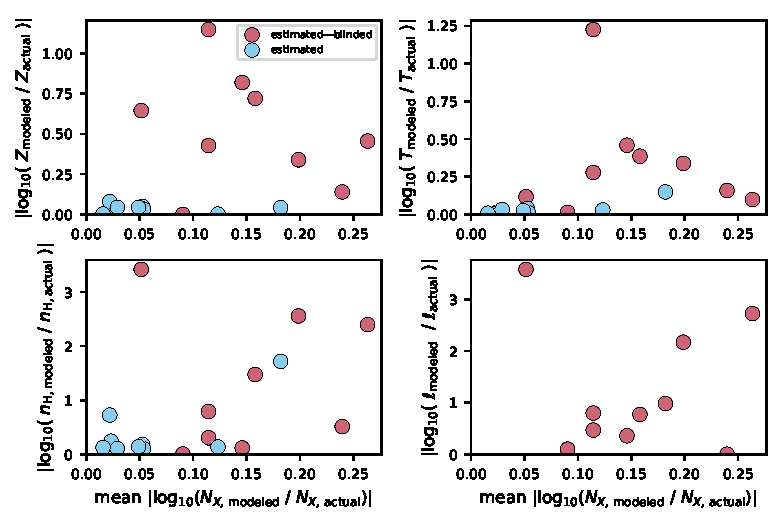
\includegraphics[width=\textwidth]{figures/sample0/error_vs_error.pdf}
    \caption{
    Error in properties of the absorbing gas vs error in column densities for \texttt{sample0}.
    The x-axis shows average log-space difference between column densities across all ions, weighted by the provided uncertainty.
    The original models fit the data decently (mean $\vert \log_{10}( N_{X,\,{\rm modeled}}$ / $N_{X,\,{\rm actual}}) \vert < 0.3$), but do not accurately recover the properties of the absorbing gas (e.g. $\vert \log_{10}( n_{\rm H,\,modeled} / n_{\rm H,\,actual}) \vert \gtrsim 1$).
    The revised models (which do not assume thermal equilibrium) recover the properties of the gas much better (e.g. $\vert \log_{10}( Z_{\rm modeled} / Z_{\rm actual}) \vert \lesssim 0.1$), and typically fit the data to mean $\vert \log_{10}( N_{X,\,{\rm modeled}}$ / $N_{X,\,{\rm actual}}) \vert \lesssim 0.05$.
    }
    \label{f: error vs error}
\end{figure*}

% Degenerate column densities
Analysis of \texttt{sample0} (\S\ref{s: results -- sample0}) suggests reasonable agreement between modeled and actual ion column densities is possible, even when the modeled temperature, density, and metallicity are inconsistent with the actual values.
We demonstrate this in Figure~\ref{f: error vs error},
which compares the per-sightline disagreement between the estimated and provided properties to the disagreement between the estimated and provided column densities, averaged across all fit ions. 
The revised estimates are in much better agreement with the actual properties, but the revised ion column densities are adjusted by only $\lesssim 0.2$ dex relative to the column densities modeled blind.
% A complicating element is that the errors theorists applied to the column densities were independent, e.g. $N_{\ion{H}{I},\,{\rm provided}} > N_{\ion{H}{I},{\rm ,actual}}$ does not mean $N_{\ion{Mg}{II},\,{\rm provided}} > N_{\ion{Mg}{II},\,{\rm actual}}$.
More broadly, this exemplifies the issue where multiple inconsistent parameter estimates provide equally good descriptions of the data.

\section{\texttt{sample2} blinded parameter estimation}
\label{a: sample2 blinded}

\begin{figure*}
    \centering
    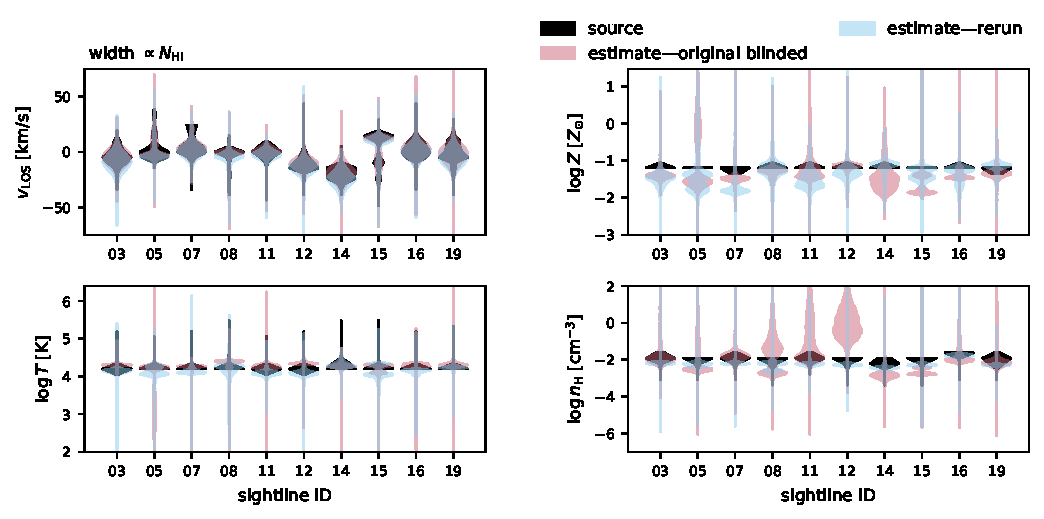
\includegraphics[width=\textwidth]{figures/sample2/violin.pdf}
    \caption{
    The distributions of $v_{\rm LOS}$, $Z$, $T$ and $n_{\rm H}$ for the synthetic source data (black) compared to the full posteriors from parameter estimation.
    The width of the violin plots scales with $N_{\ion{H}{I}}$.
    The posteriors for both the blinded and revised parameter estimations overlap with the source distributions in most cases, suggesting the parameter estimation is typically sufficiently conservative.
    Exceptions are
    both the blinded and revised posteriors of $Z$ for \texttt{07},
    the blinded posteriors of $Z$ for \texttt{14} and \texttt{15},
    most of the blinded posteriors of $T$,
    and both the blinded and revised posteriors of $n_{\rm H}$ for \texttt{12}, \texttt{14}, and \texttt{15}.
    }
    \label{f: sample2 violin both}
\end{figure*}


\begin{figure*}
    \centering
    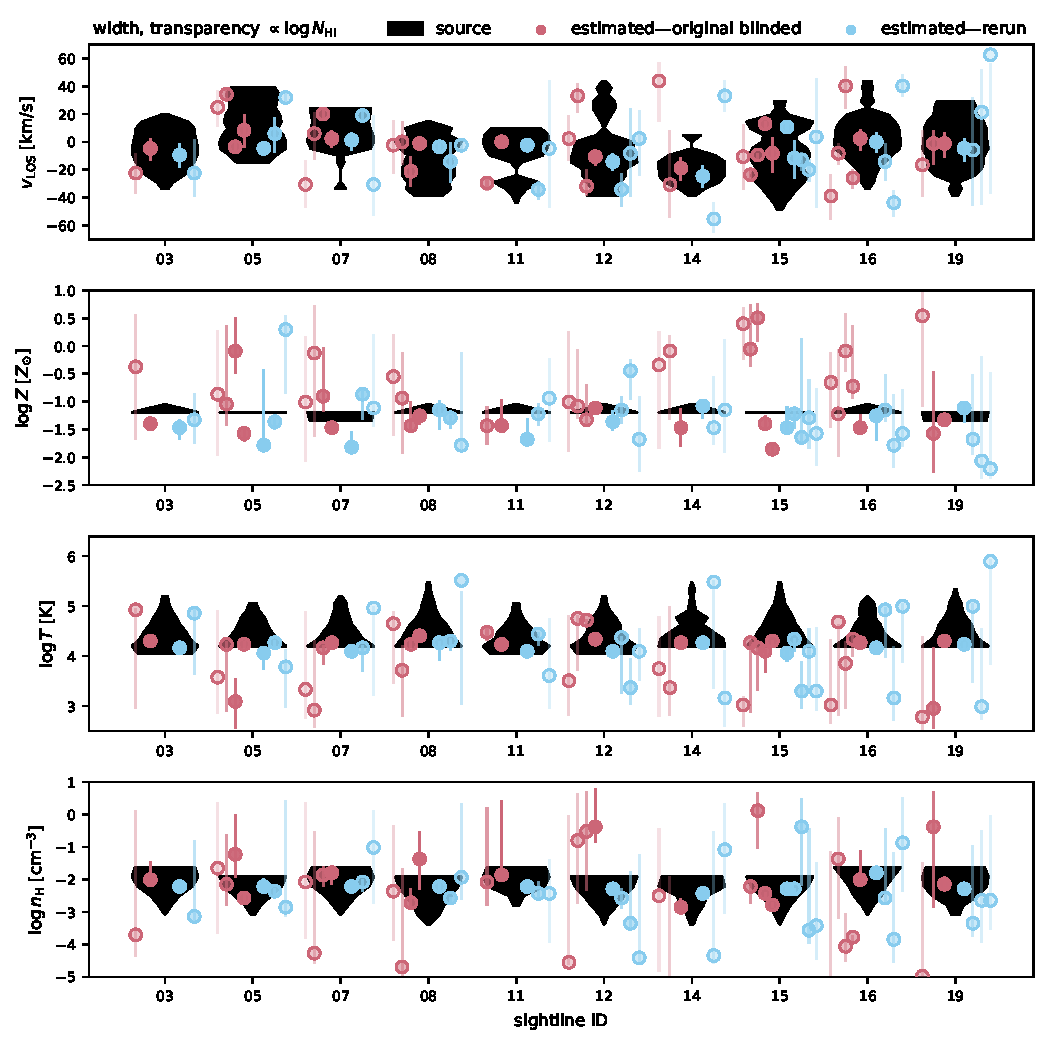
\includegraphics[width=\textwidth]{figures/sample2/violin_vs_components.pdf}
    \caption{
    The distributions of $v_{\rm LOS}$, $Z$, $T$ and $n_{\rm H}$ for the synthetic source data (black) compared to the best estimates for individual components comprising the parameter estimation.
    Each point is the maximum-likelihood estimate (MLE) of an individual component,
    and the associated bars enclose the the 16th to 84th percentiles of the posterior.
    The width of the violin plots and the opacity of the points are scaled \textit{logarithmically} with $N_{\ion{H}{I}}$,
    such that if the parameter estimation perfectly agreed with the data all visible MLE points would lie within the source data violins.
    The MLE of the strongest component typically aligns with the peak of the source distribution, but can be off by $\lesssim 1$ dex for $Z$ and $n_{\rm H}$, especially for the blinded estimates.
    The best fit for parameter estimation consistently includes lower-column-density components with properties not found in the source data.
    }
    \label{f: sample2 violin vs components both}
\end{figure*}

% Blinded sample
The primary difference between the blinded and revised estimates lies in the source data and the employed UVB,
rather than the estimation methodology.
The temperature, density, metallicity, LOS velocity, and total column for \texttt{sample2} were extracted from $z=2$ sightlines passing through a high-resolution simulation of a turbulent mixing zone.
To avoid providing any hints about the origin of the data the synthetic generators aimed to provide $z \sim 0 - 0.25$ spectra,
as was done for the preceding samples.
To this end, for the blinded \texttt{sample2} the synthetic generators took the $z=2$ absorbing-gas properties,
generated spectra using the $z=0.13$ UV ionization table,
and provided synthetic observations mimicking COS observations of gas at $z=0.13$.
The concept was to generate absorption from $z=0.13$ gas,
independent of the mechanisms responsible for setting the properties of the gas.

% Revised sample
The revised \texttt{sample2} synthetic spectra used a $z=2$ ionization table,
had a wavelength resolution of 0.05 \AA,
a line spread function with a FWHM of 7 km/s,
and included the ions \ion{H}{I}, \ion{Si}{II}, \ion{Si}{III}, \ion{Si}{IV}, \ion{C}{II}, \ion{C}{III}, \ion{C}{IV}, \ion{O}{I}, \ion{O}{VI}, \ion{N}{II}, \ion{N}{V}, \ion{Fe}{II}, \ion{Mg}{X}, and \ion{Ne}{VIII}.
The ($Z$, $n_{\rm H}$, $T$, $\NHI$) of the source data were not modified.
These changes followed discussion between the theorists and observers.
The better agreement between the revised parameter estimation and the source properties is likely related to the changes in the provided spectra.
For example, the blinded estimates of $T$ are consistently high by $\sim 0.1$ dex,
while the revised estimates agree better.

\section{Sightline-by-sightline comparisons for \texttt{sample2}}
\label{a: all sightlines for sample2}

\begin{figure*}
    \centering
    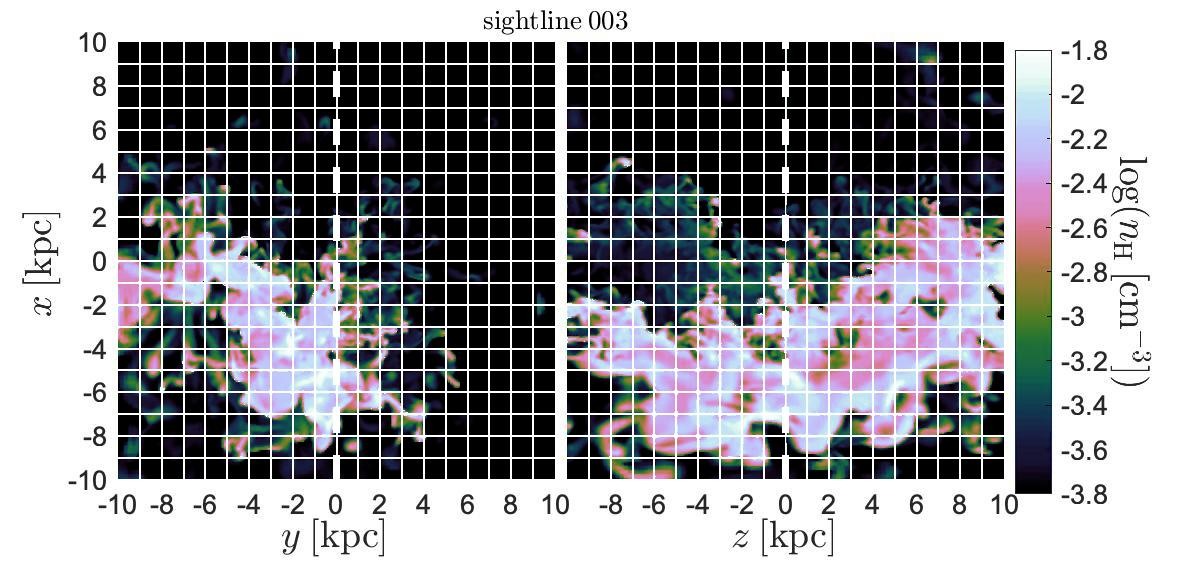
\includegraphics[width=0.49\textwidth]{figures/sample2/projections/density_projection_maps_SL_03.jpg}
    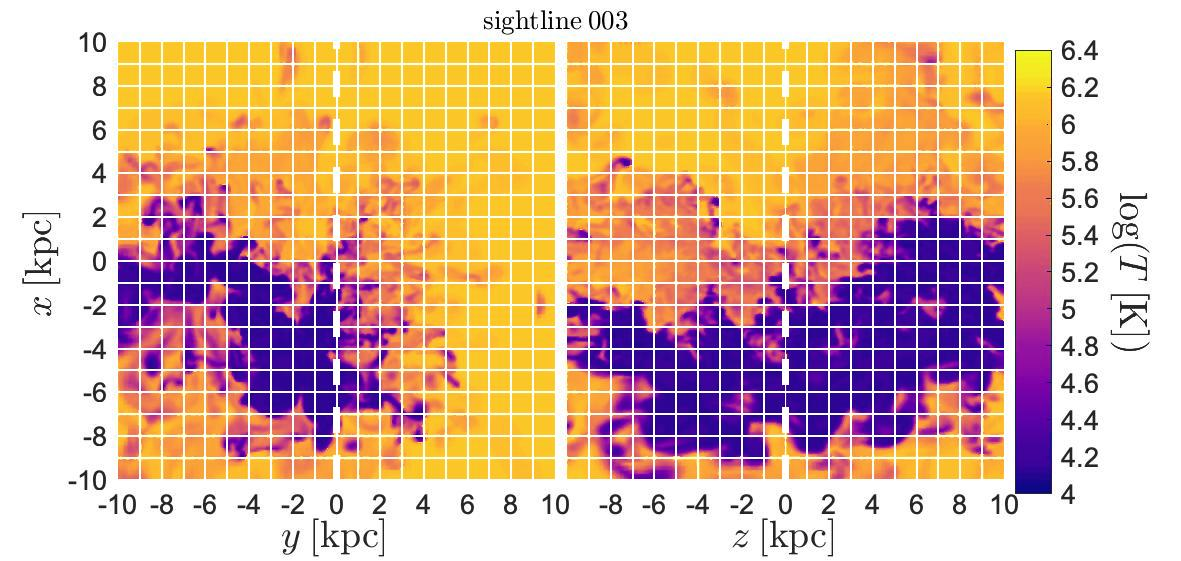
\includegraphics[width=0.49\textwidth]{figures/sample2/projections/temperature_projection_maps_SL_03.jpg} \\
    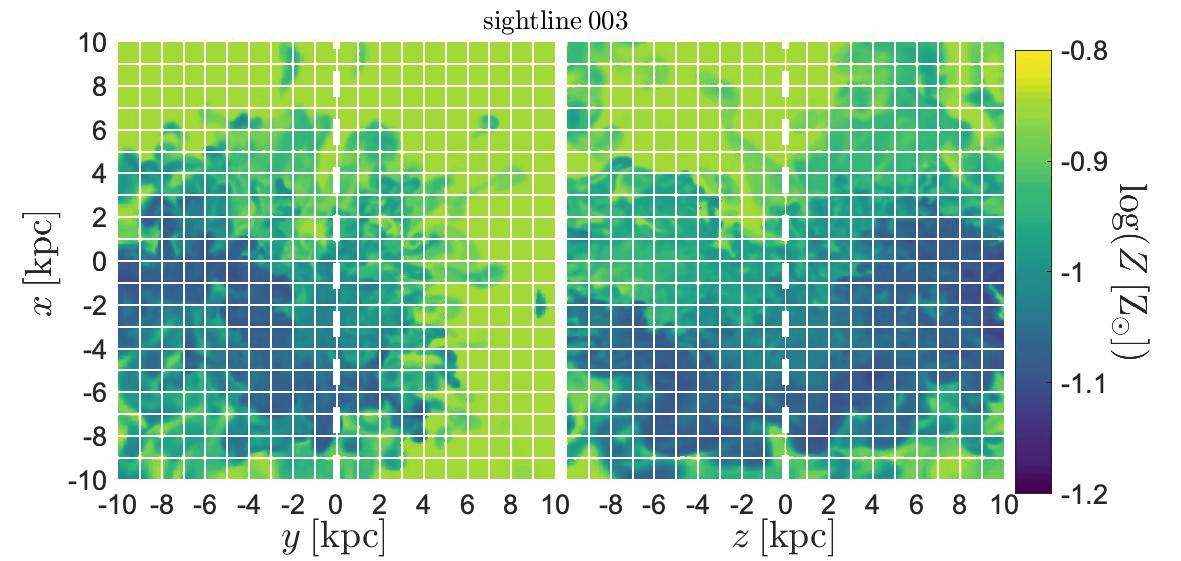
\includegraphics[width=0.49\textwidth]{figures/sample2/projections/metallicity_projection_maps_SL_03.jpg}
    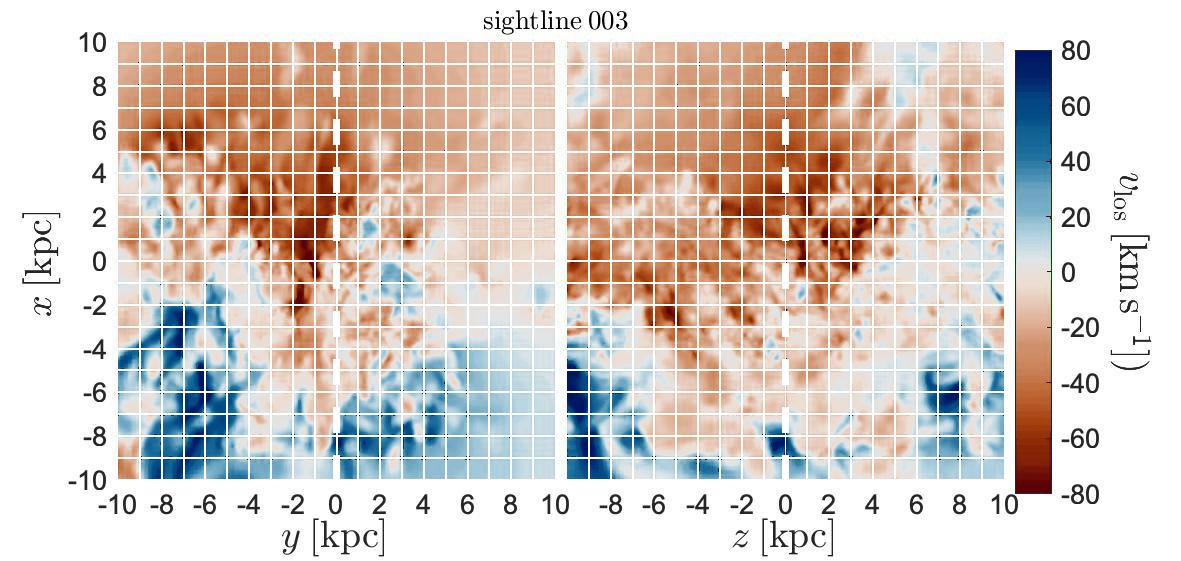
\includegraphics[width=0.49\textwidth]{figures/sample2/projections/velocity_projection_maps_SL_03.jpg}
    \caption{
    Density, temperature, metallicity, and line-of-sight velocity in a slice of the simulation used to generate \texttt{sample2}~\citep{mandelker2020Instability}.
    The dashed white line shows the location of one of the sightlines (sightline 03) forward-modeled to produce mock spectra.
    }
    \label{f: sample2 ray 03}
\end{figure*}

\begin{figure*}
    \centering
    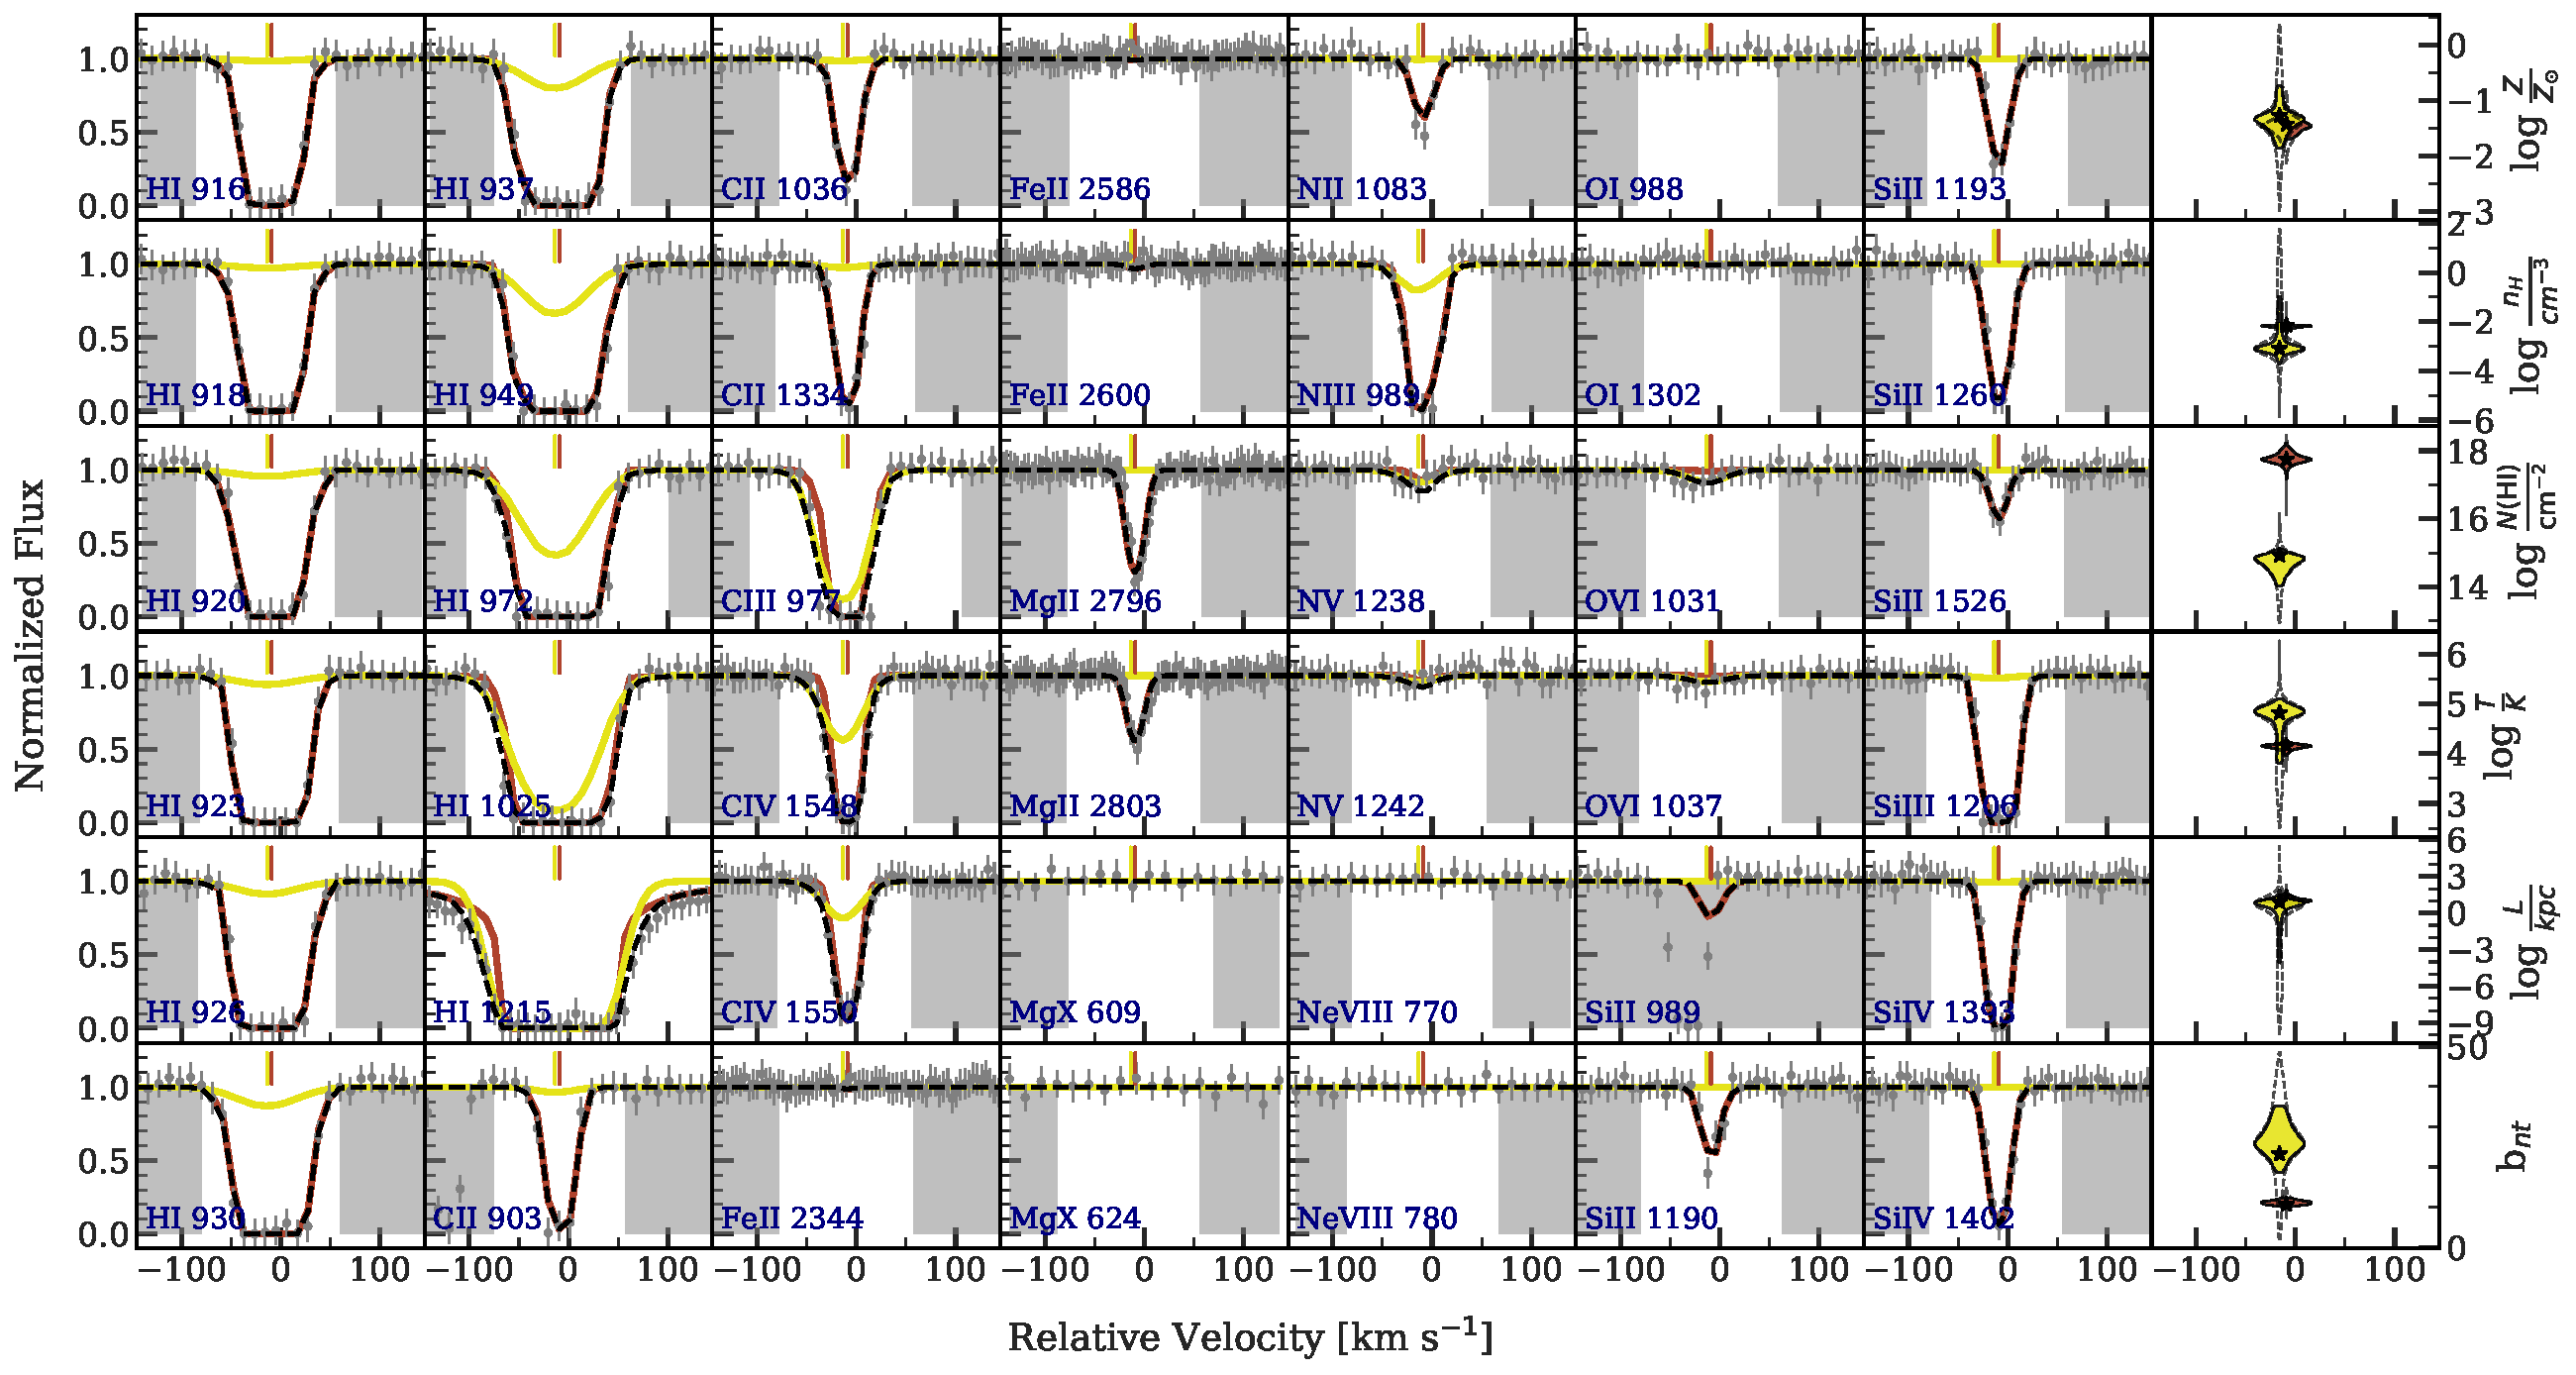
\includegraphics[width=\textwidth]{figures/sample2/best_fits/0003.pdf}
    \caption{
    Mock spectra for sightline 03,
    best fit absorption profiles found by observers,
    and the parameters of the best fits.
    }
    \label{f: sample2 spectrum 03}
\end{figure*}

\begin{figure*}
    \centering
    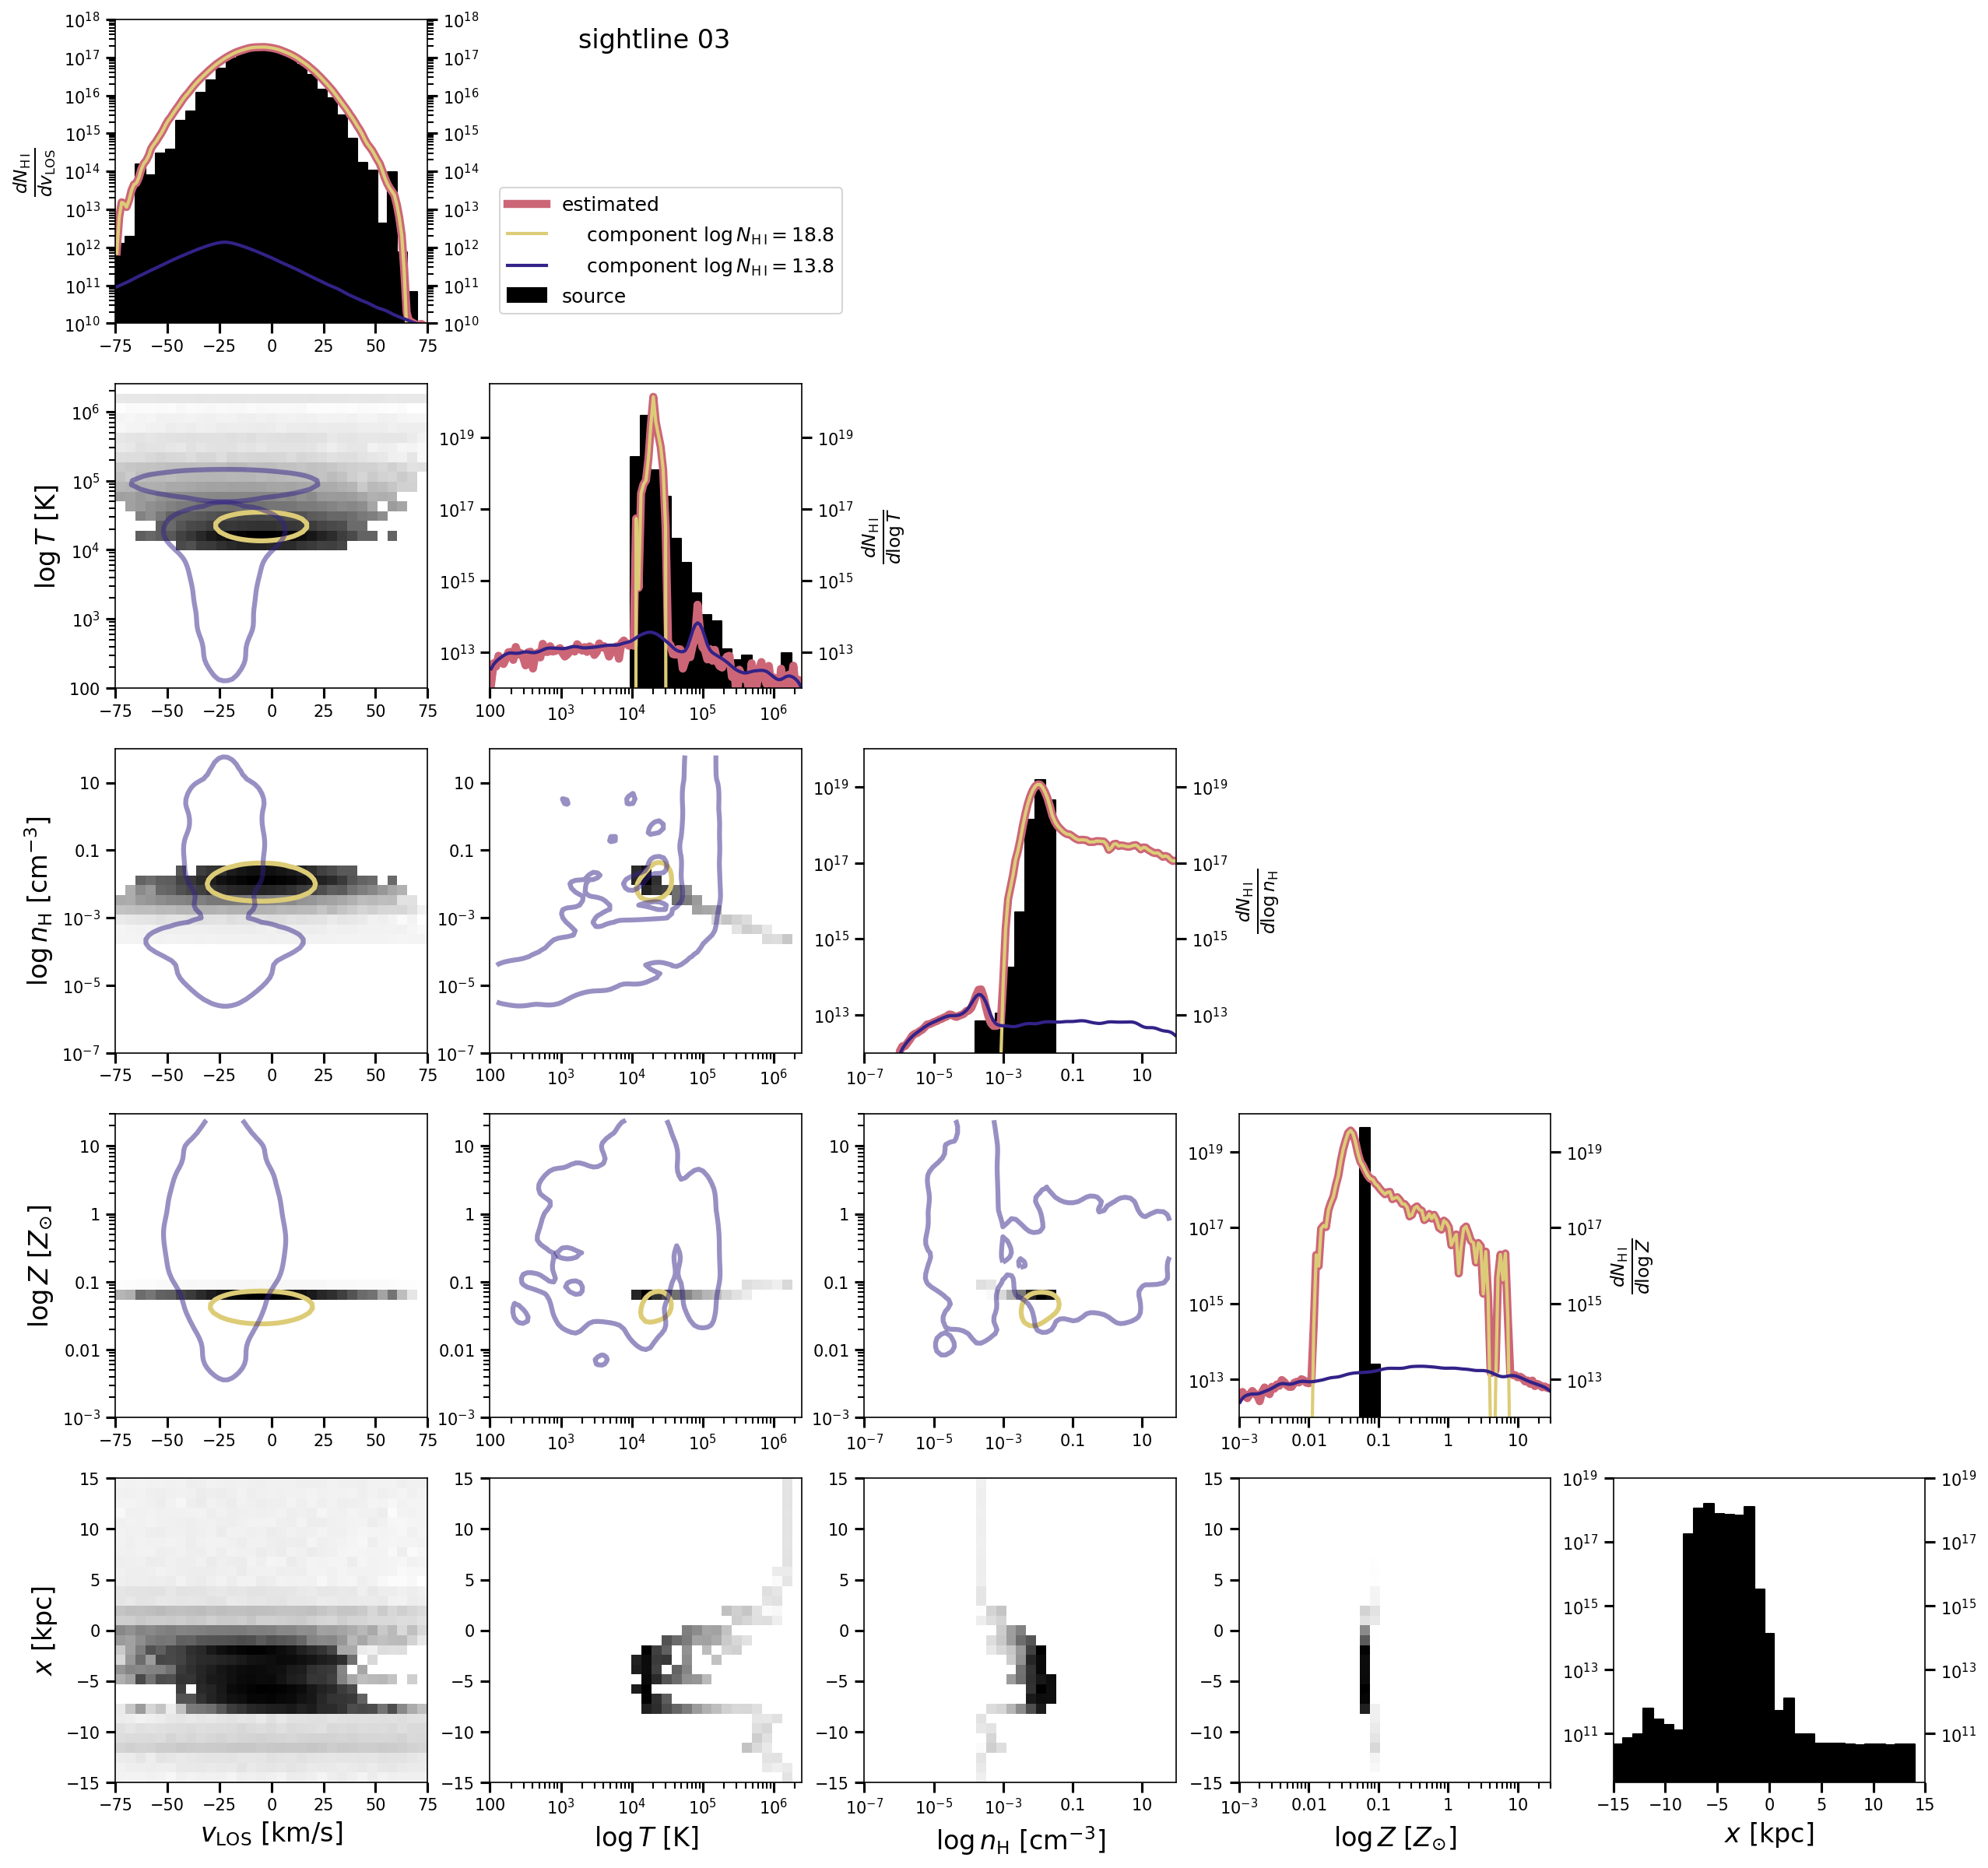
\includegraphics[height=0.45\textheight]{figures/sample2/original/sightline_0003.png}
    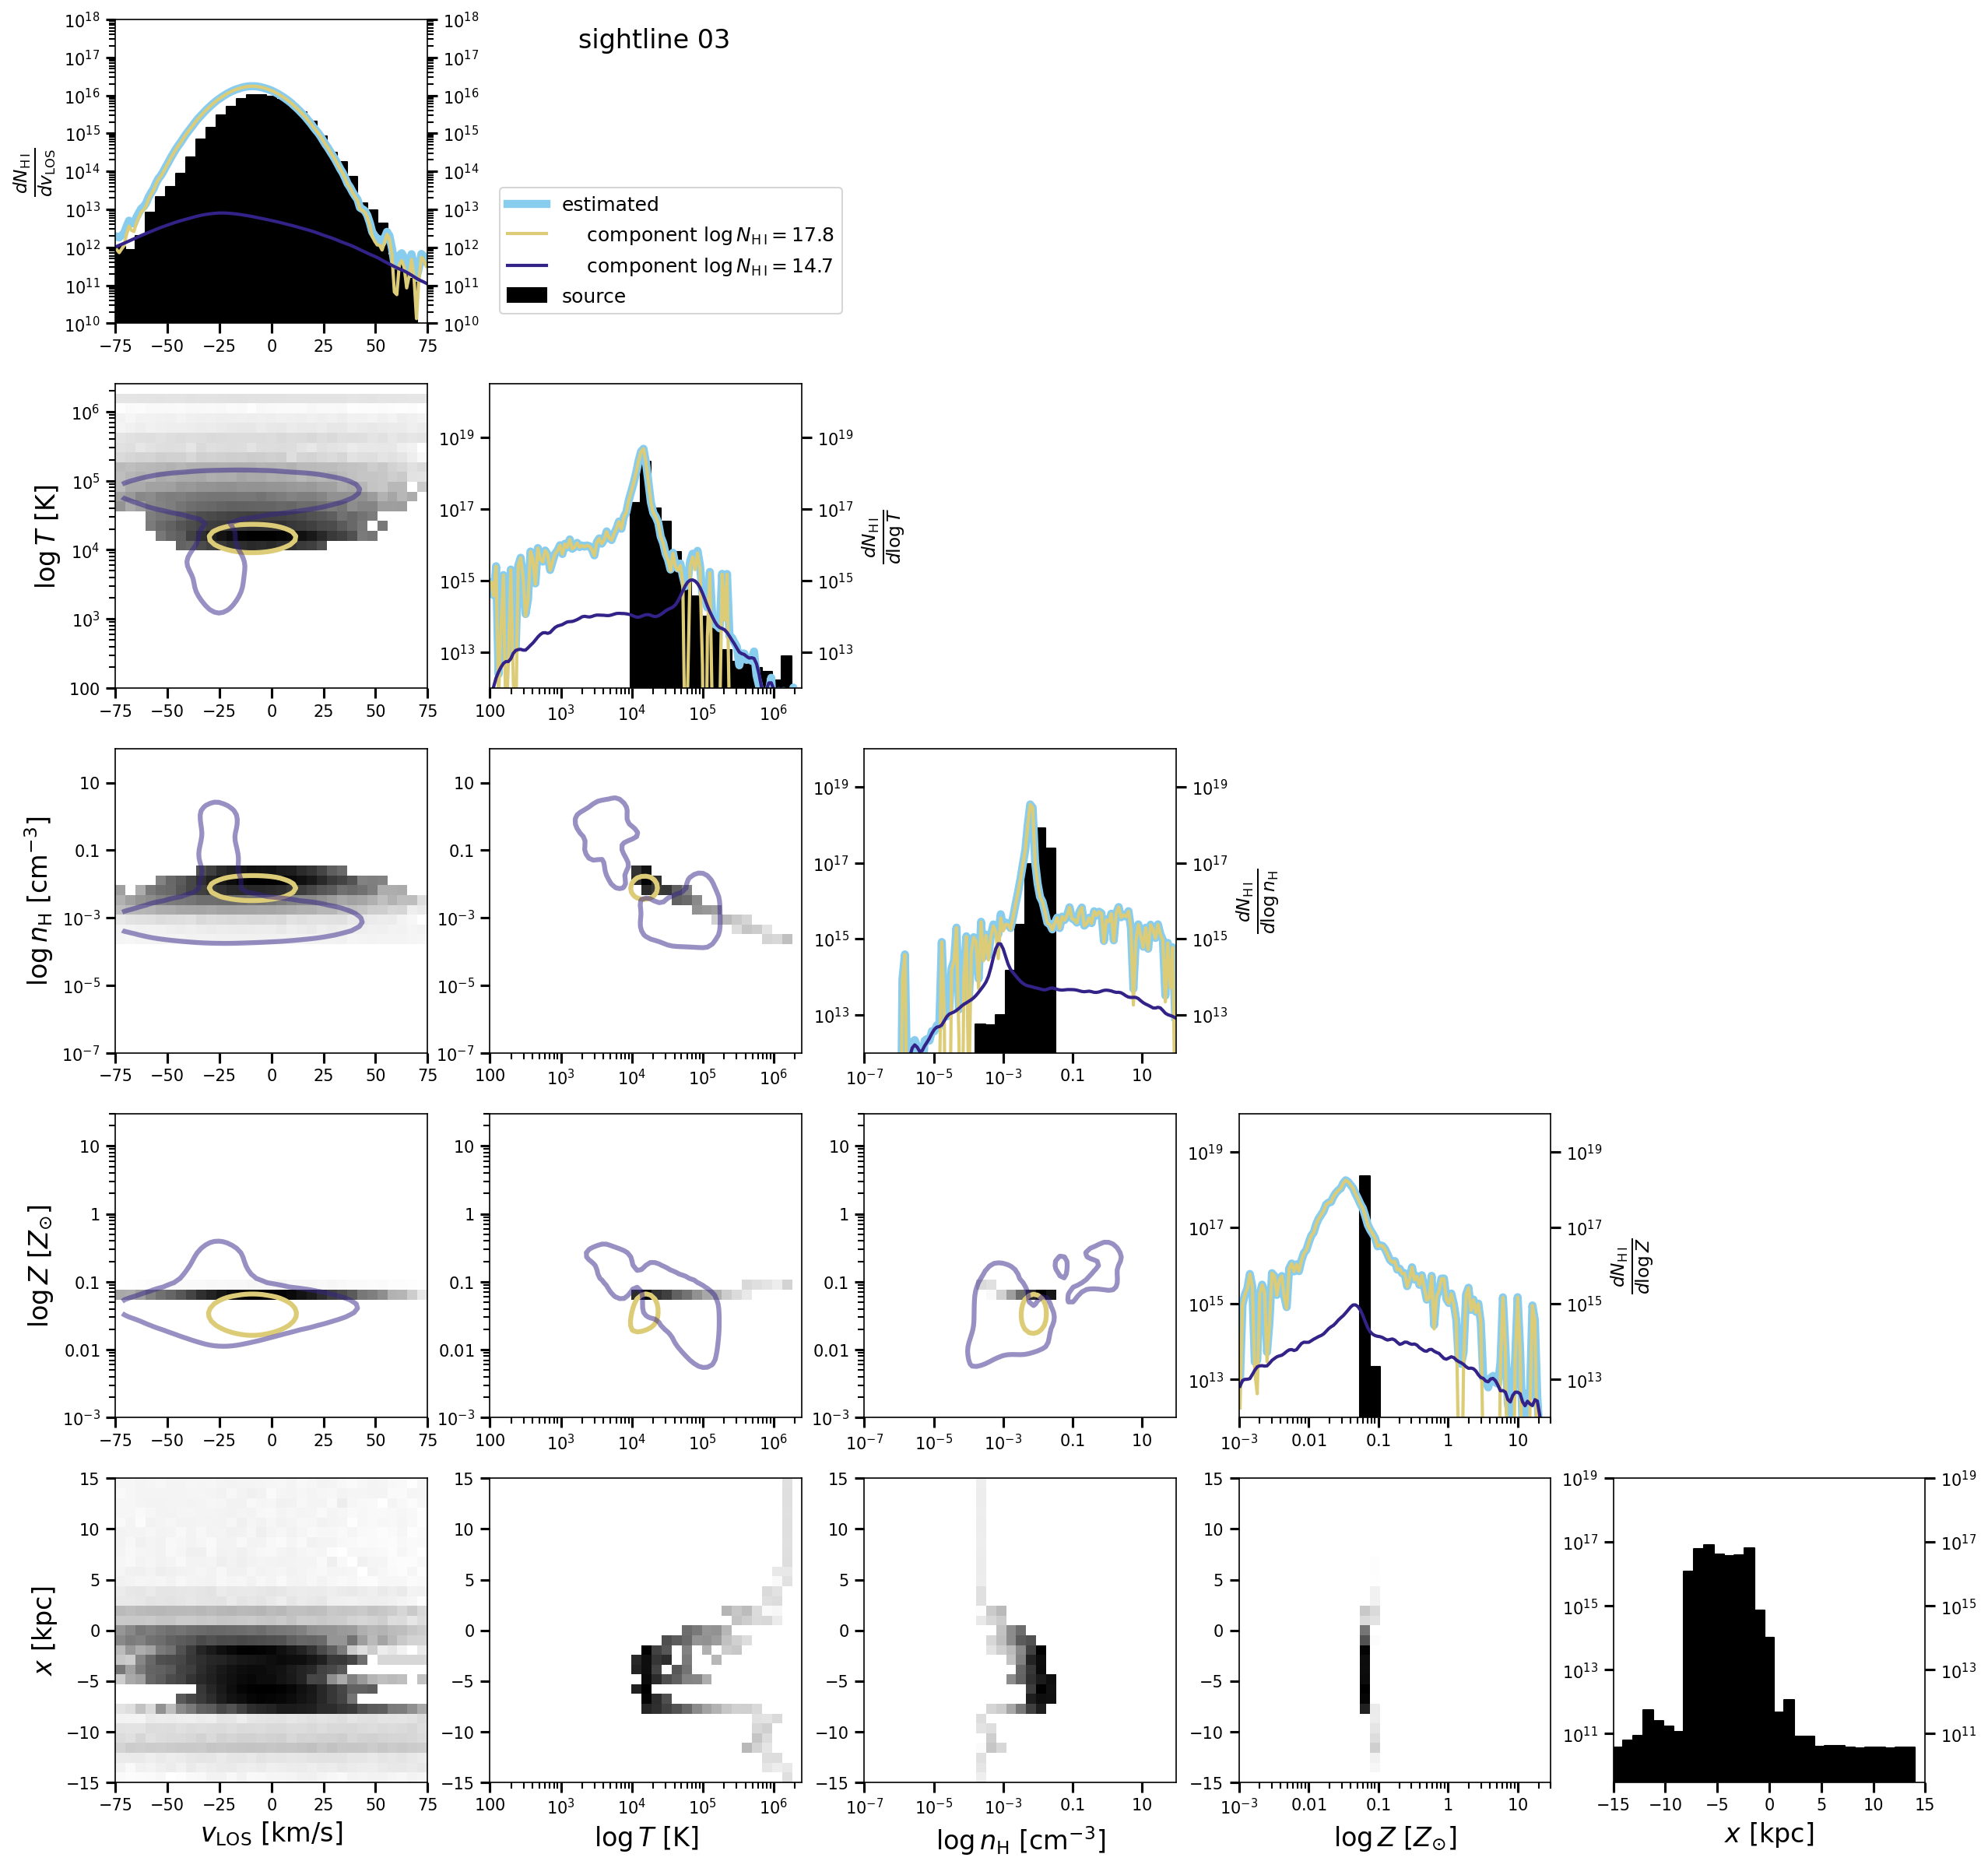
\includegraphics[height=0.45\textheight]{figures/sample2/high-z/sightline_0003.png}
    \caption{Corner plot for sightline 03.}
    \label{f: sample2 corner 03}
\end{figure*}

\begin{figure*}
    \centering
    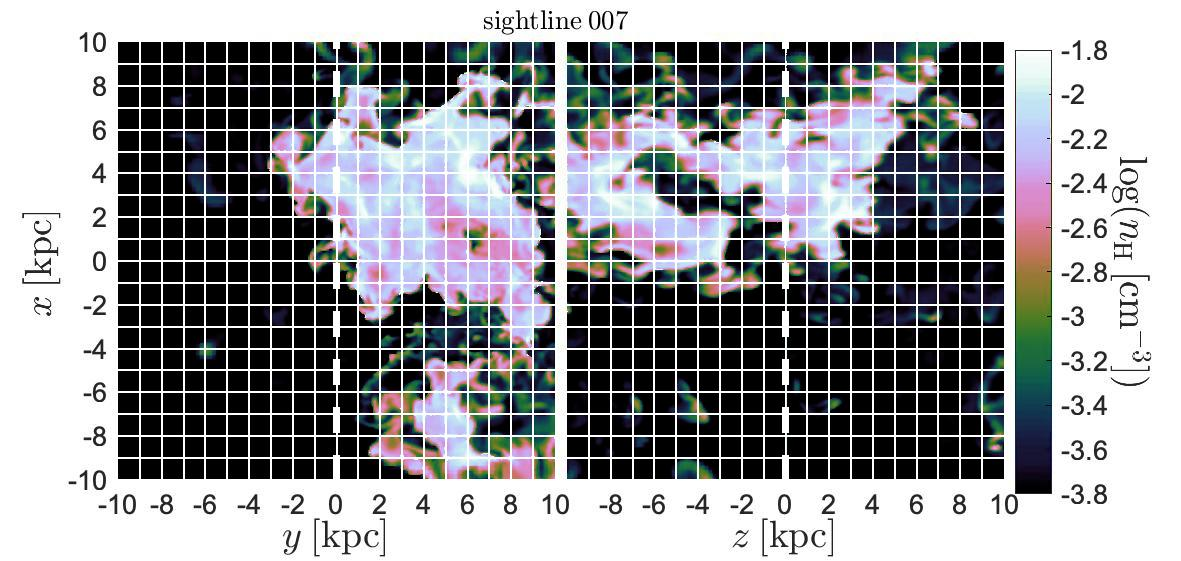
\includegraphics[width=0.49\textwidth]{figures/sample2/projections/density_projection_maps_SL_07.jpg}
    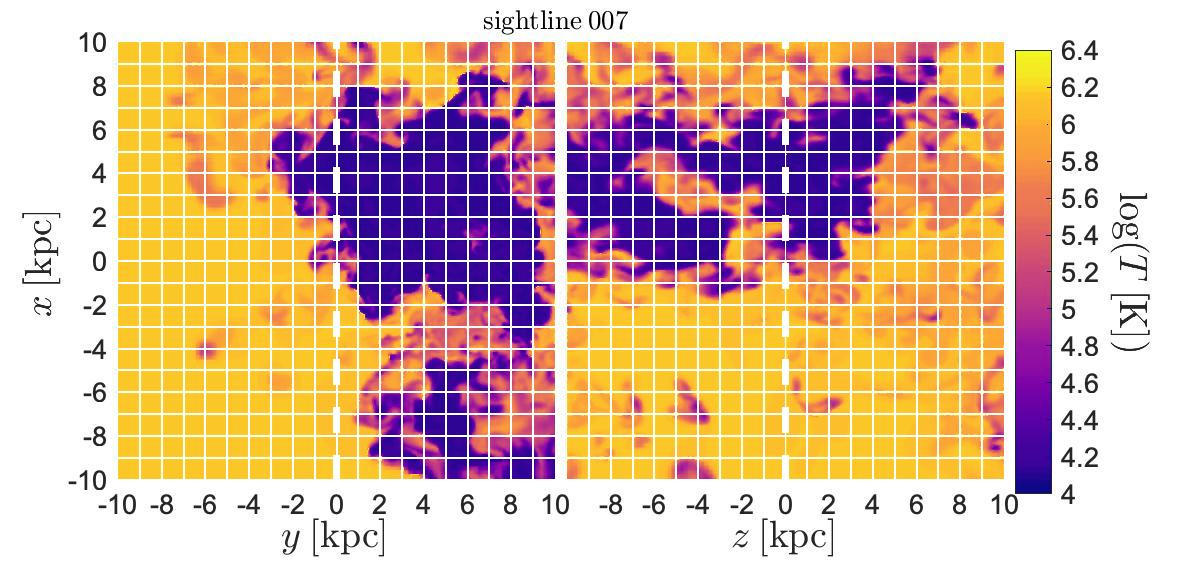
\includegraphics[width=0.49\textwidth]{figures/sample2/projections/temperature_projection_maps_SL_07.jpg} \\
    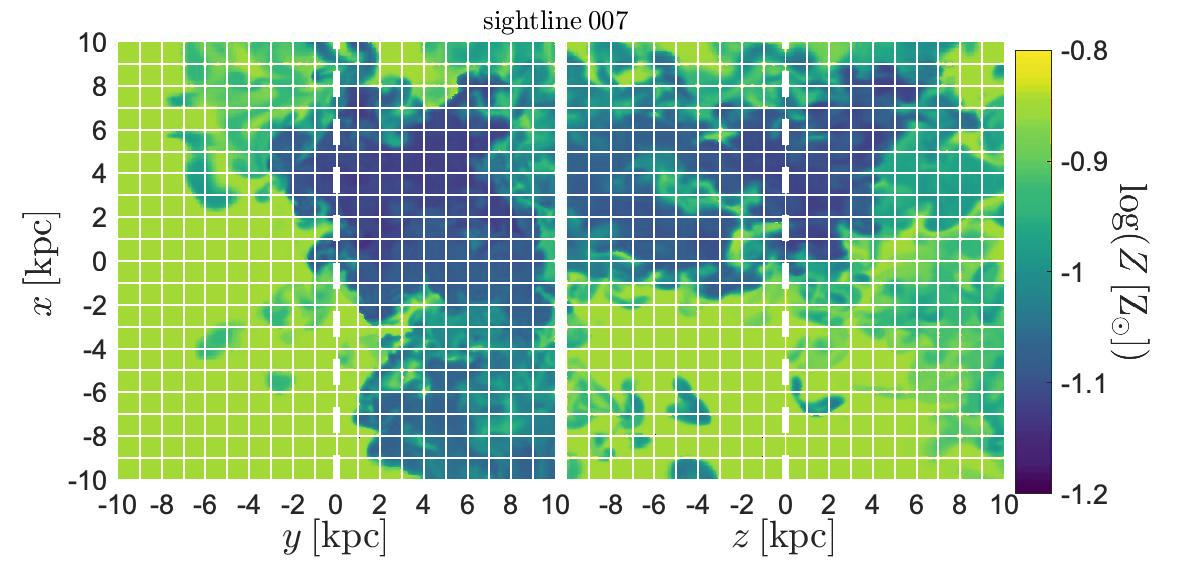
\includegraphics[width=0.49\textwidth]{figures/sample2/projections/metallicity_projection_maps_SL_07.jpg}
    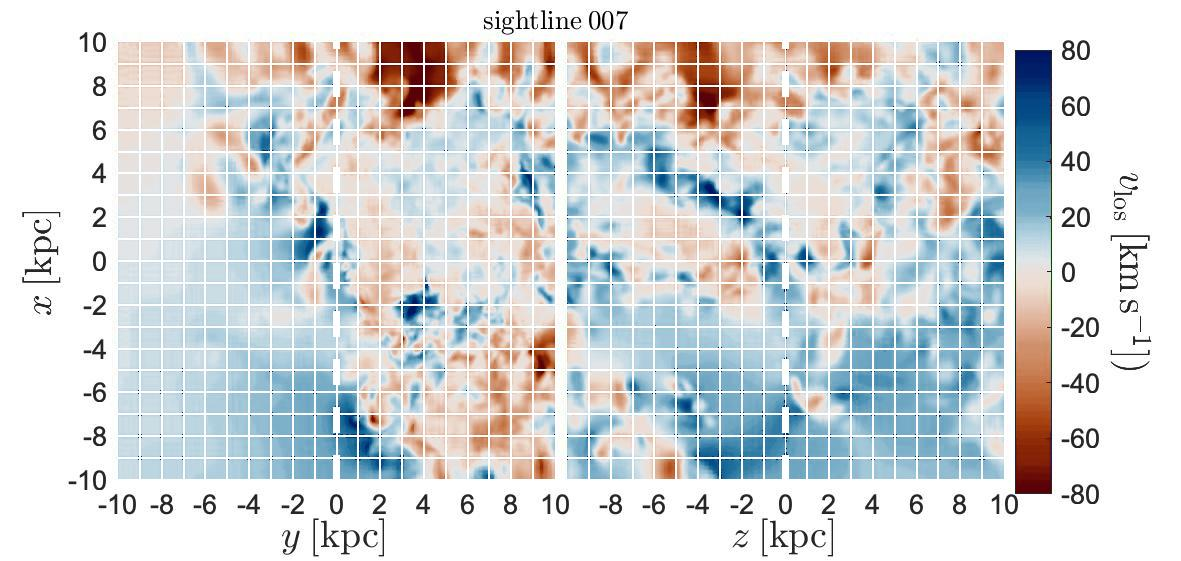
\includegraphics[width=0.49\textwidth]{figures/sample2/projections/velocity_projection_maps_SL_07.jpg}
    \caption{
    Density, temperature, metallicity, and line-of-sight velocity in a slice of the simulation used to generate \texttt{sample2}~\citep{mandelker2020Instability}.
    The dashed white line shows the location of one of the sightlines (sightline 07) forward-modeled to produce mock spectra.
    }
    \label{f: sample2 ray 07}
\end{figure*}

\begin{figure*}
    \centering
    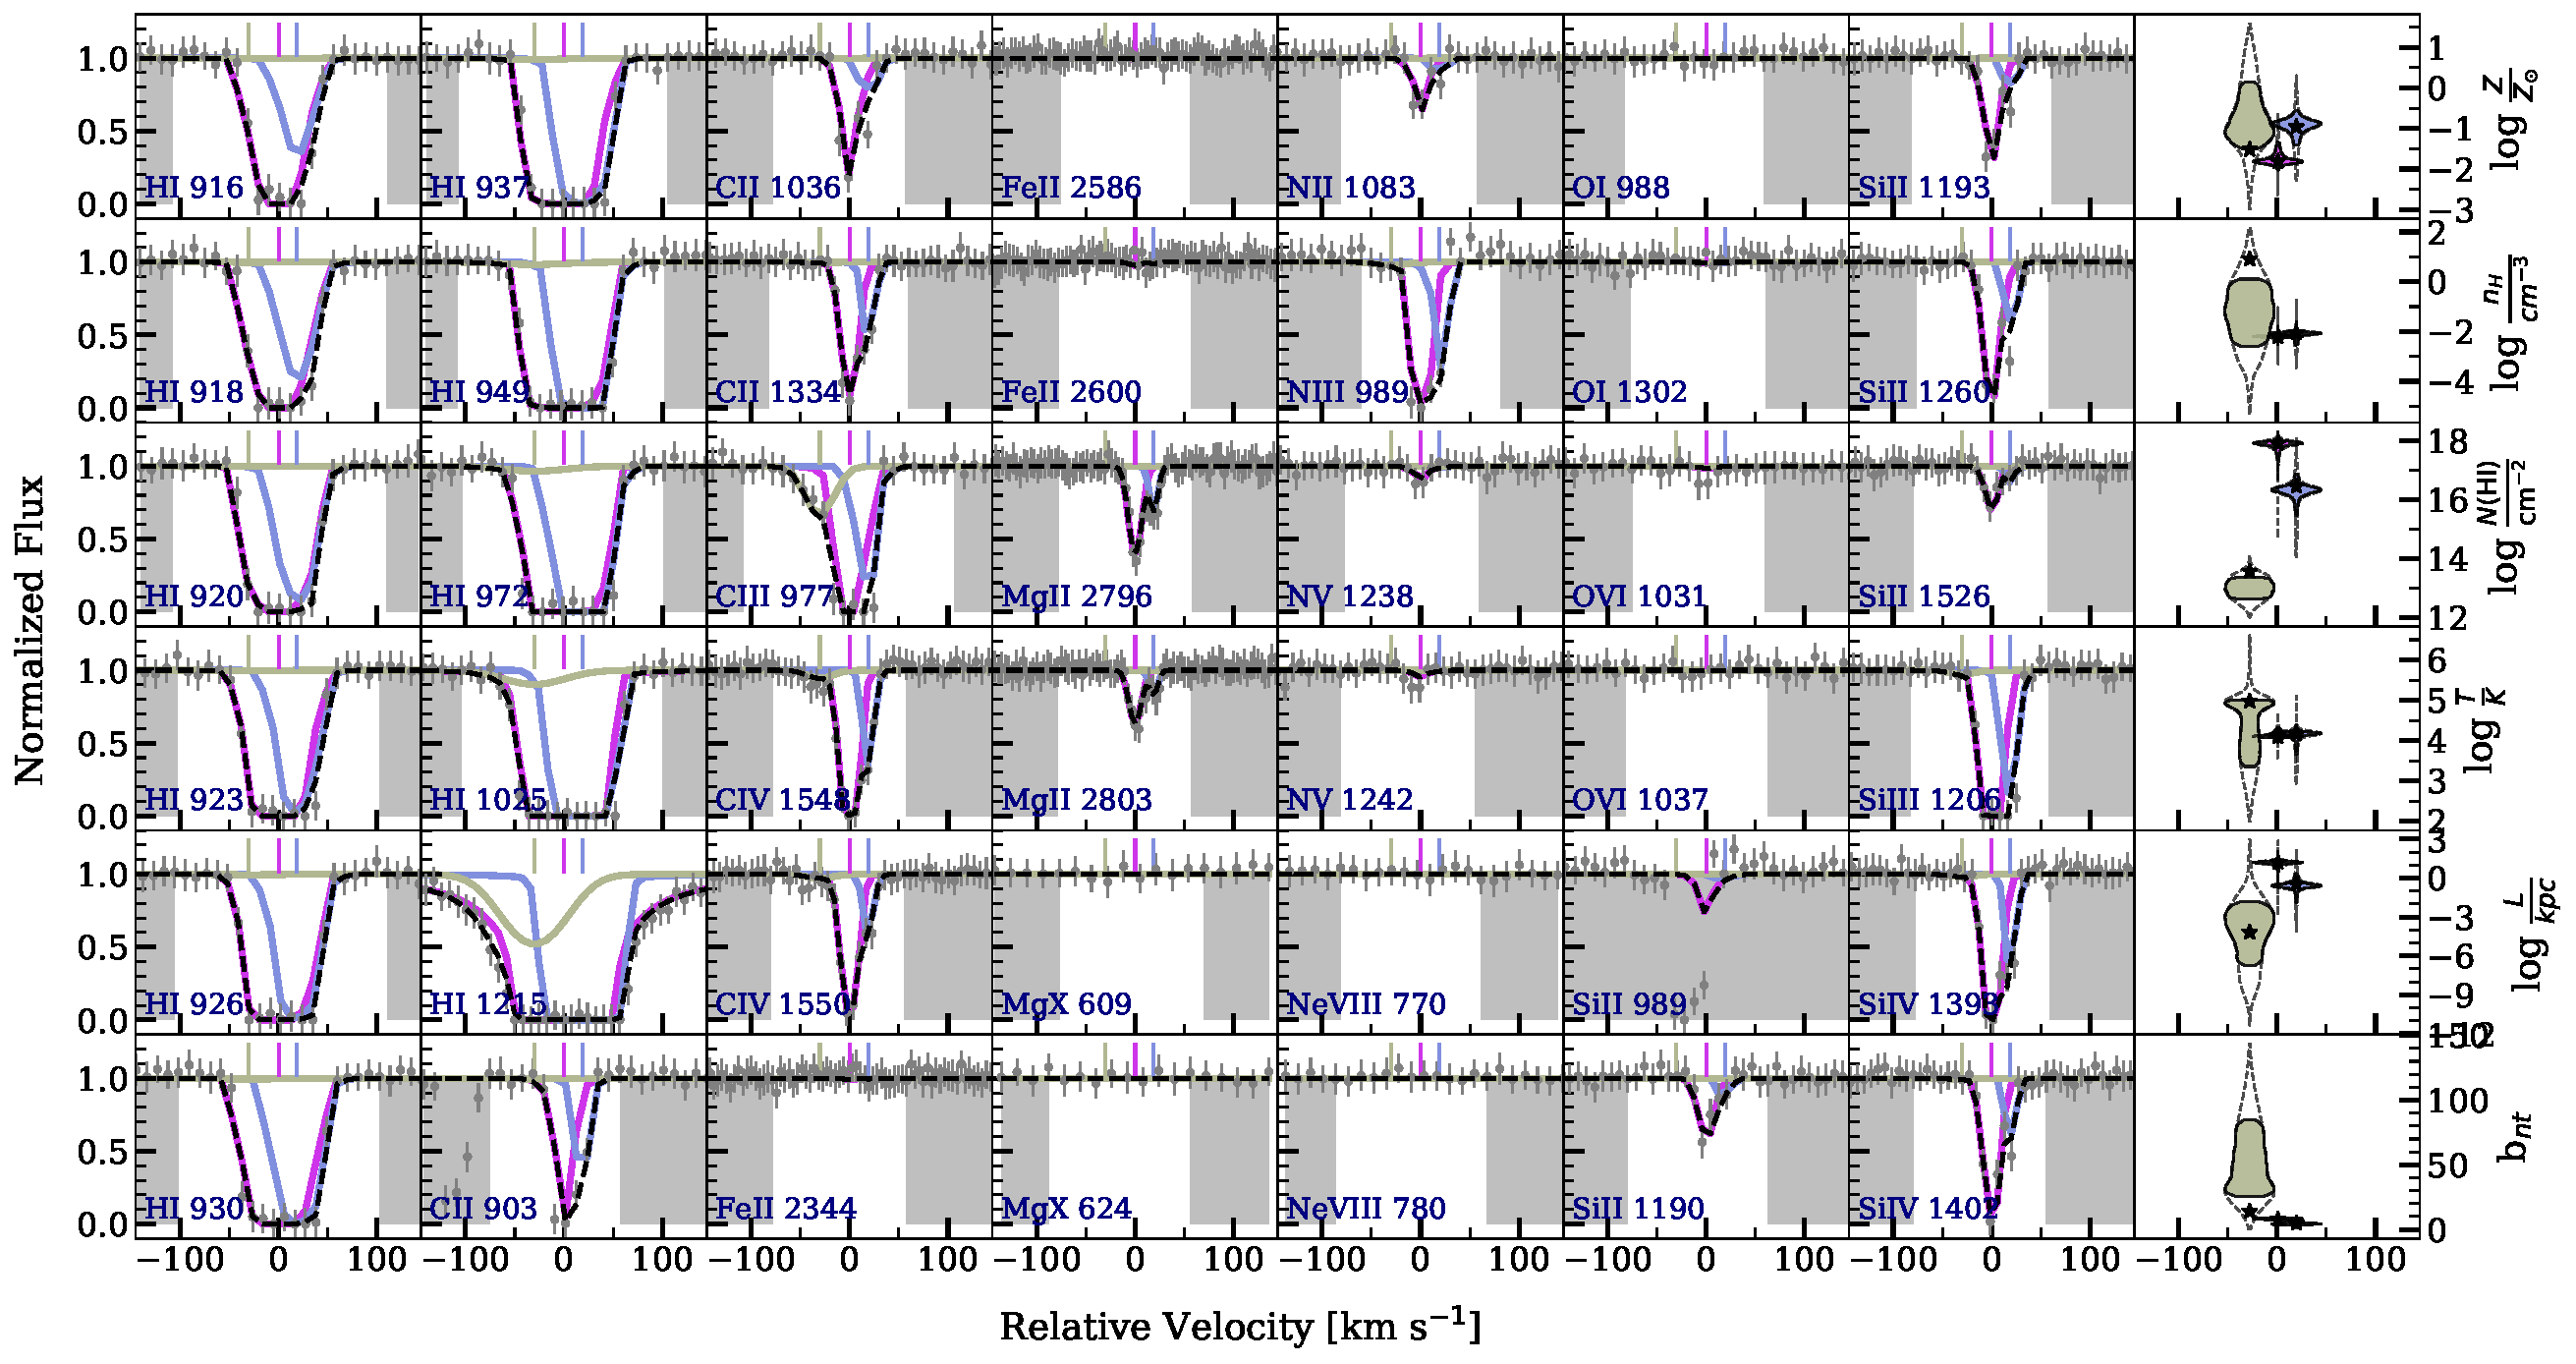
\includegraphics[width=\textwidth]{figures/sample2/best_fits/0007.pdf}
    \caption{
    Mock spectra for sightline 07,
    best fit absorption profiles found by observers,
    and the parameters of the best fits.
    }
    \label{f: sample2 spectrum 07}
\end{figure*}

\begin{figure*}
    \centering
    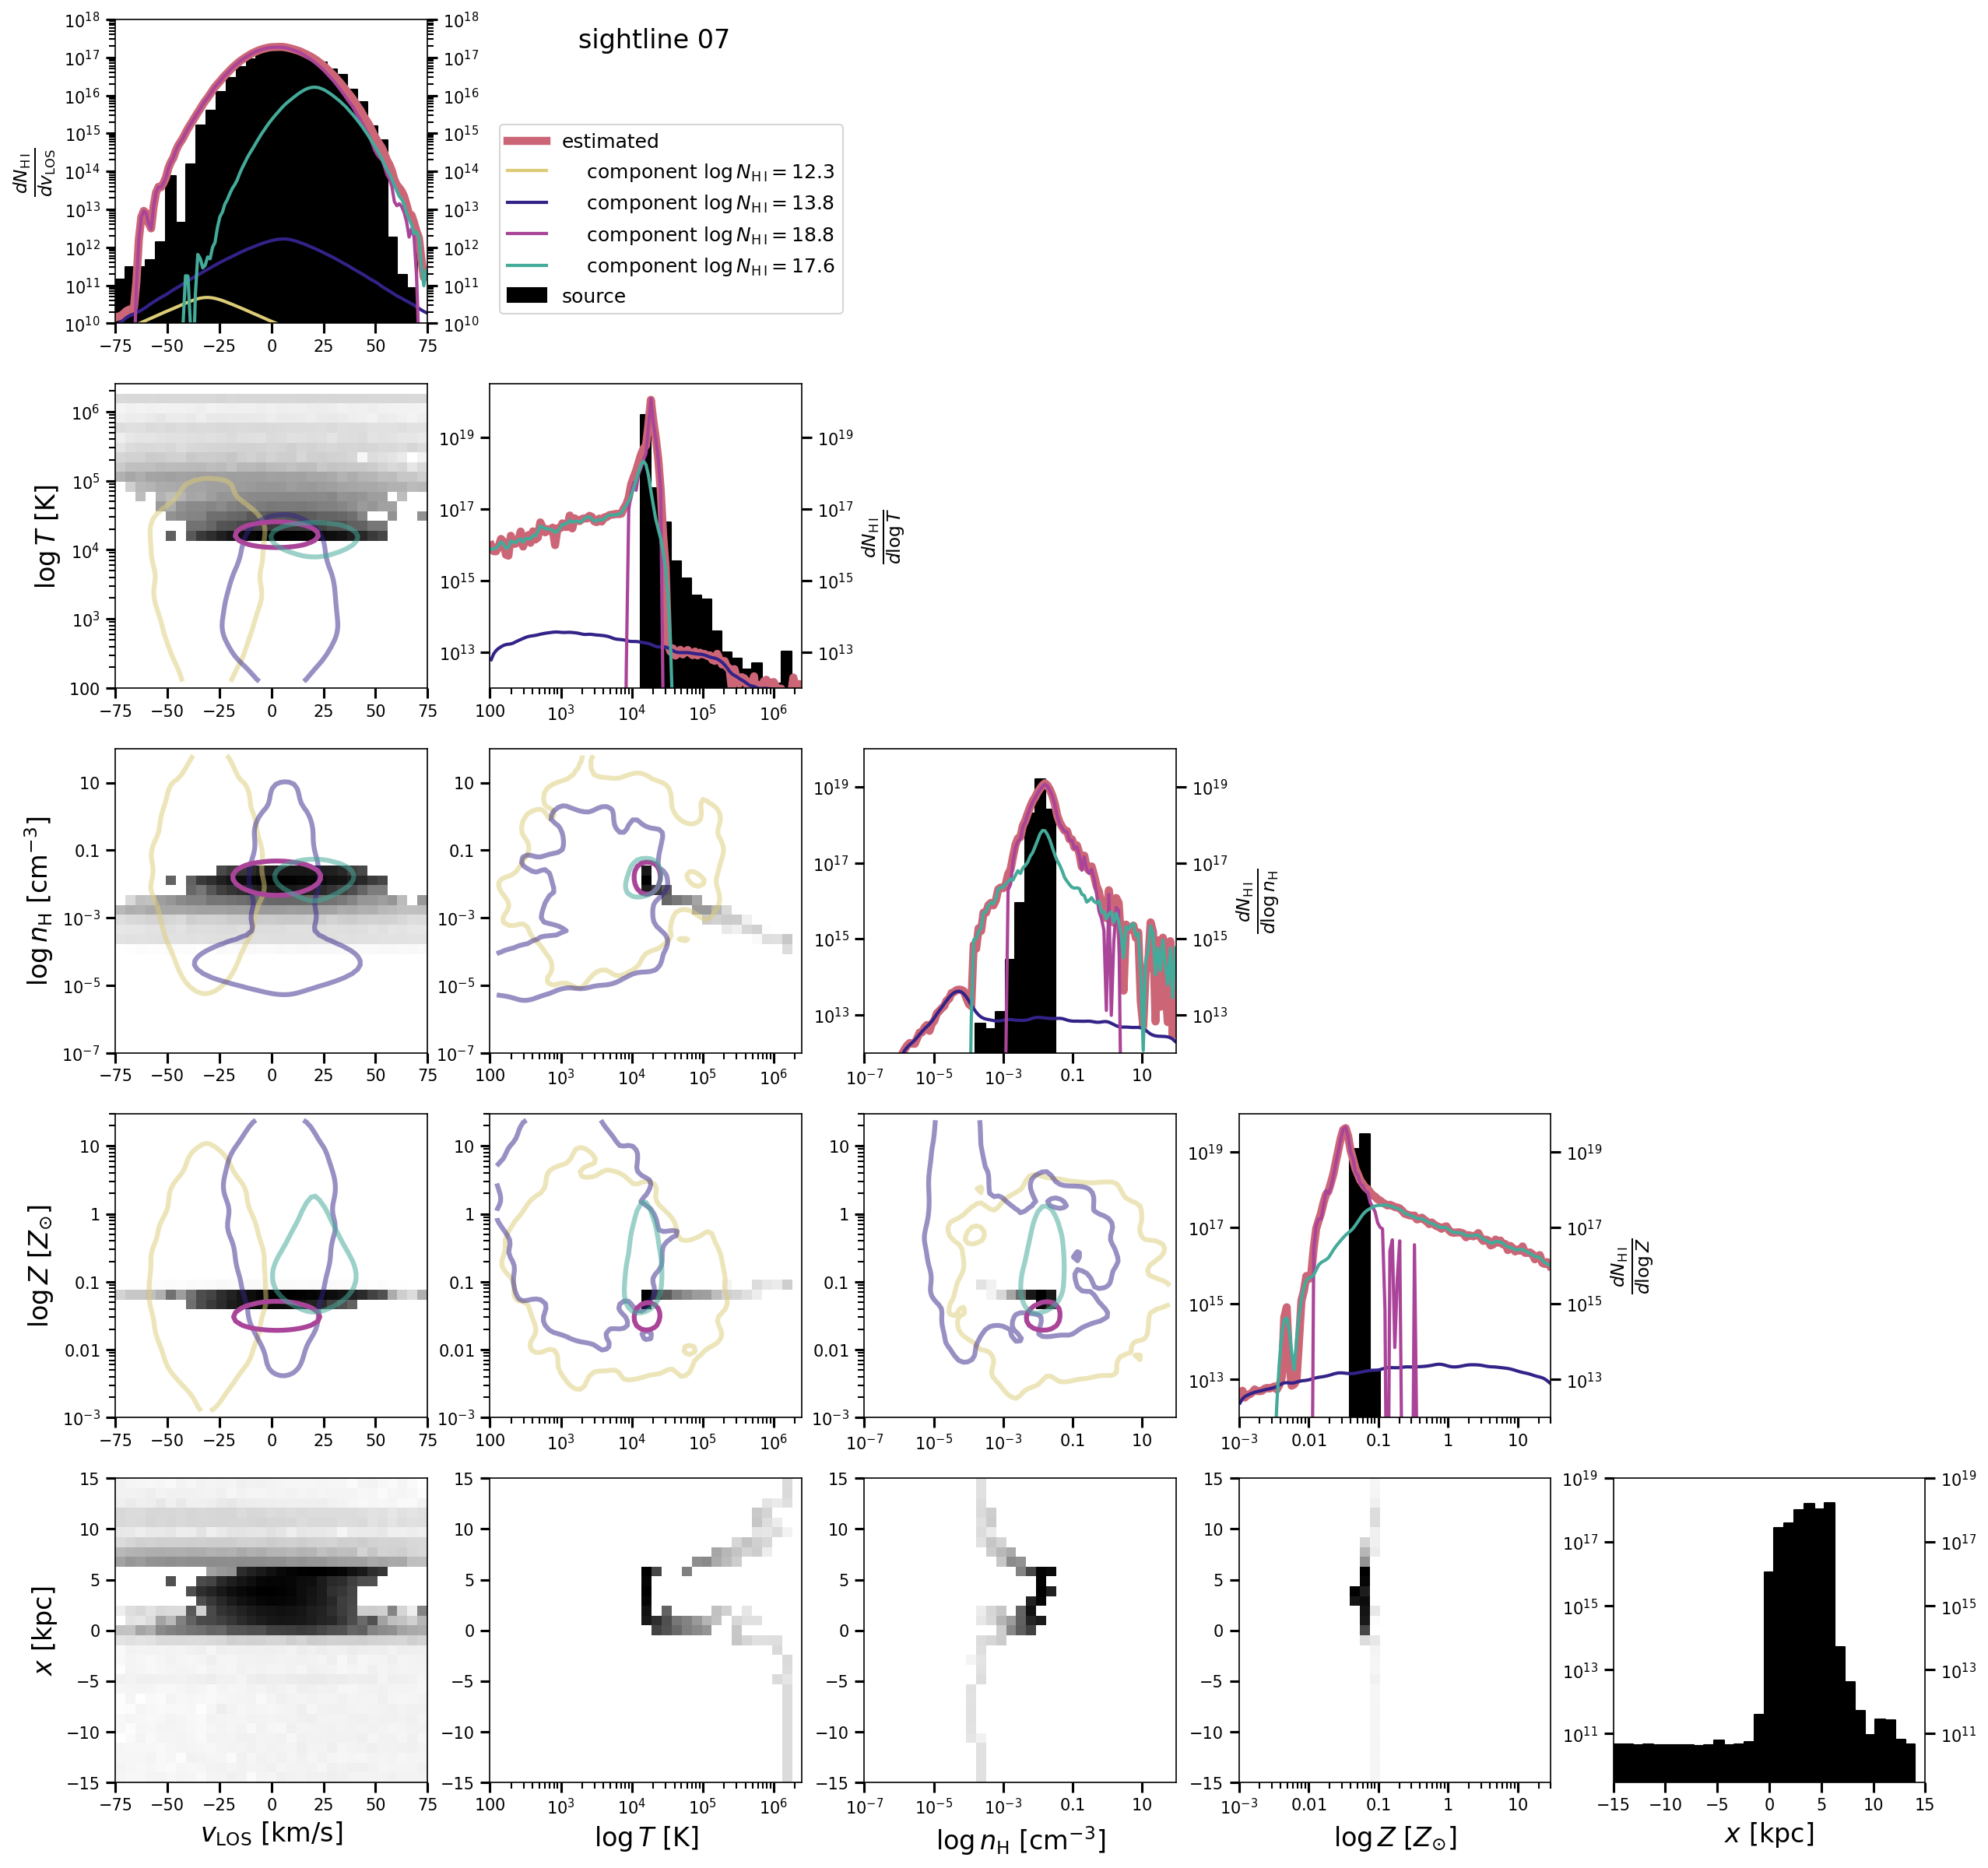
\includegraphics[height=0.45\textheight]{figures/sample2/original/sightline_0007.png}
    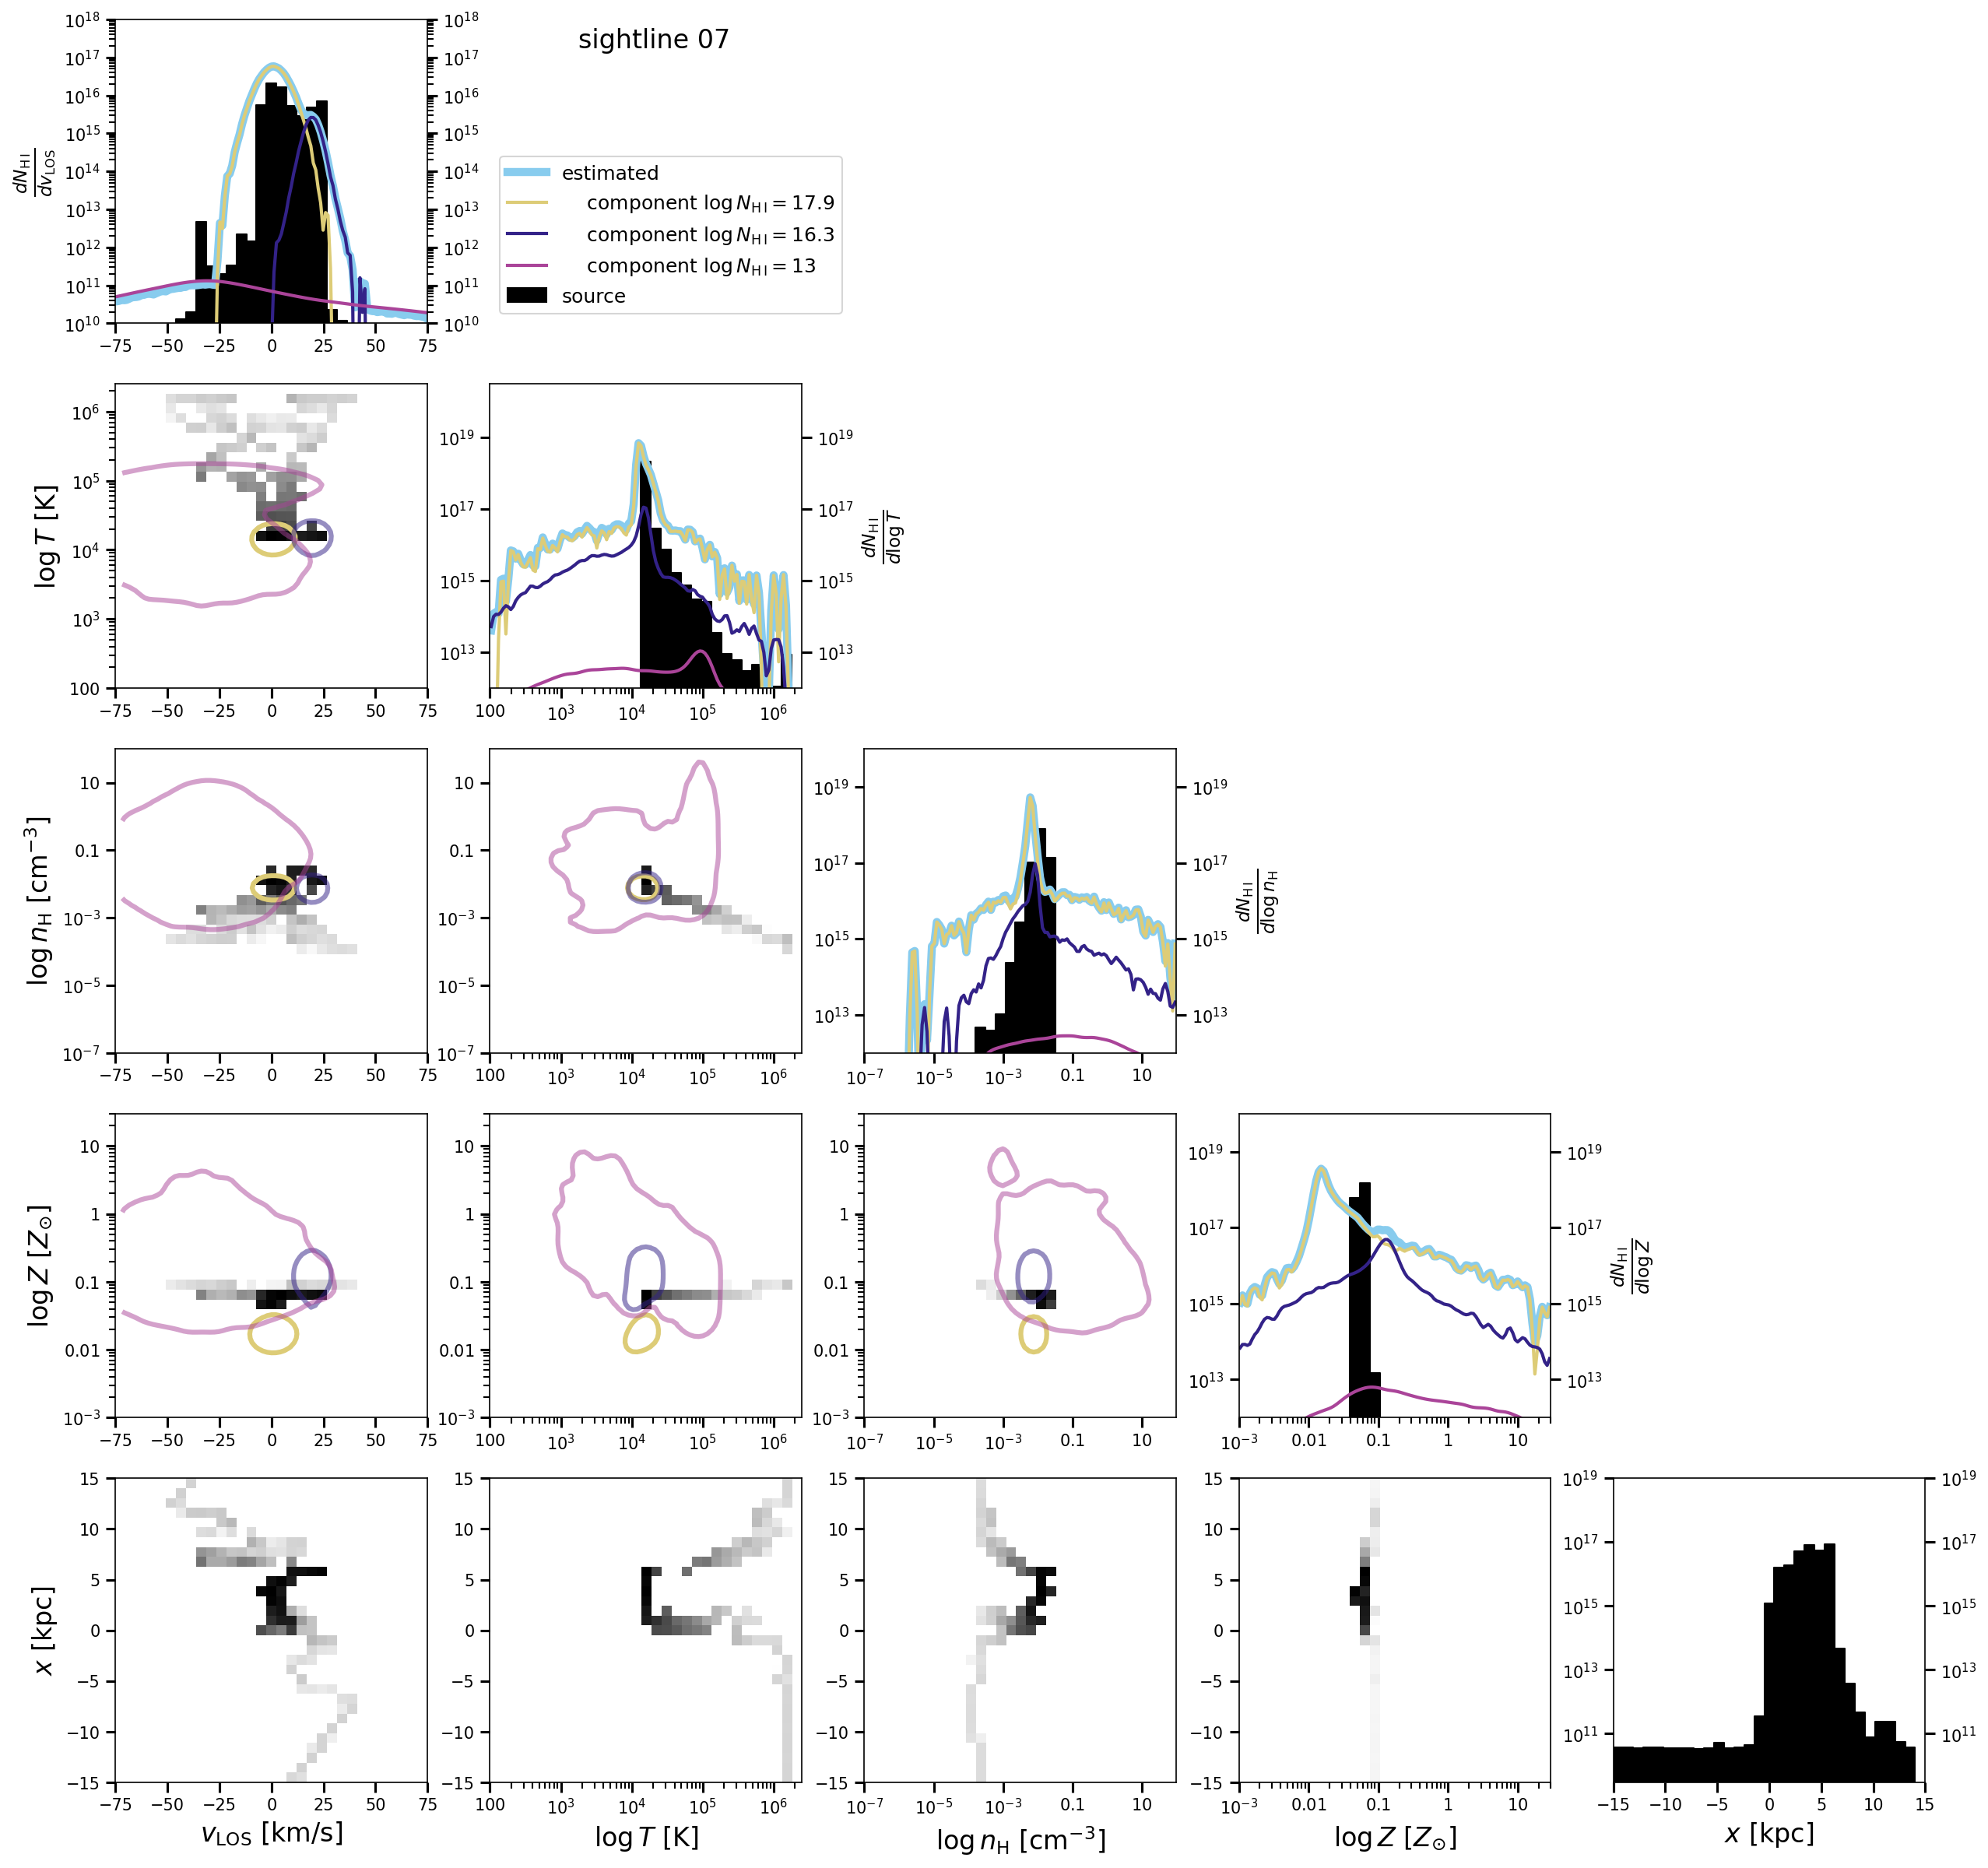
\includegraphics[height=0.45\textheight]{figures/sample2/high-z/sightline_0007.png}
    \label{f: sample2 07 corner}
    \caption{Same as Fig.~\ref{f: sample2 corner 03}, but for sightline 07.}
\end{figure*}

\begin{figure*}
    \centering
    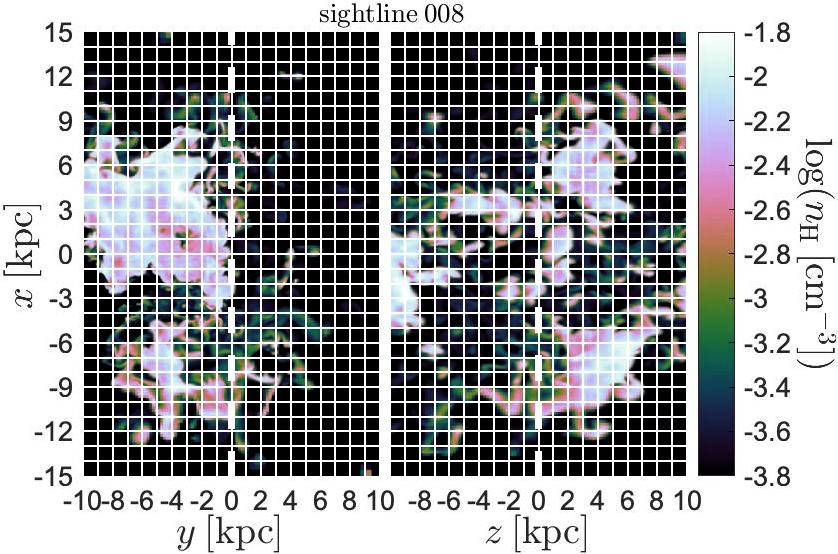
\includegraphics[width=0.49\textwidth]{figures/sample2/projections/density_projection_maps_SL_08.jpg}
    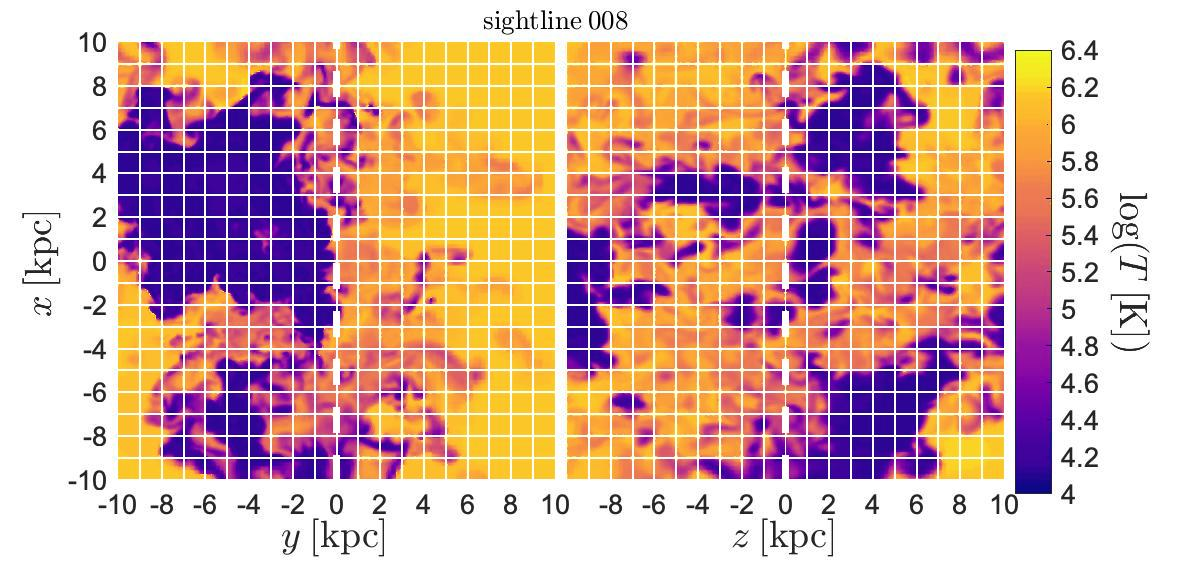
\includegraphics[width=0.49\textwidth]{figures/sample2/projections/temperature_projection_maps_SL_08.jpg} \\
    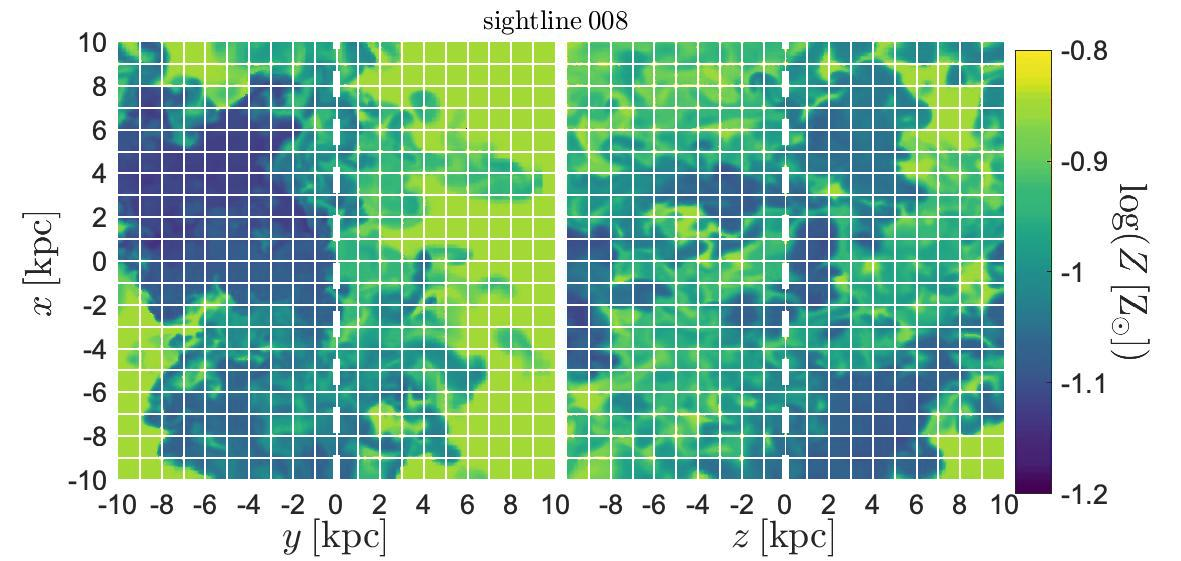
\includegraphics[width=0.49\textwidth]{figures/sample2/projections/metallicity_projection_maps_SL_08.jpg}
    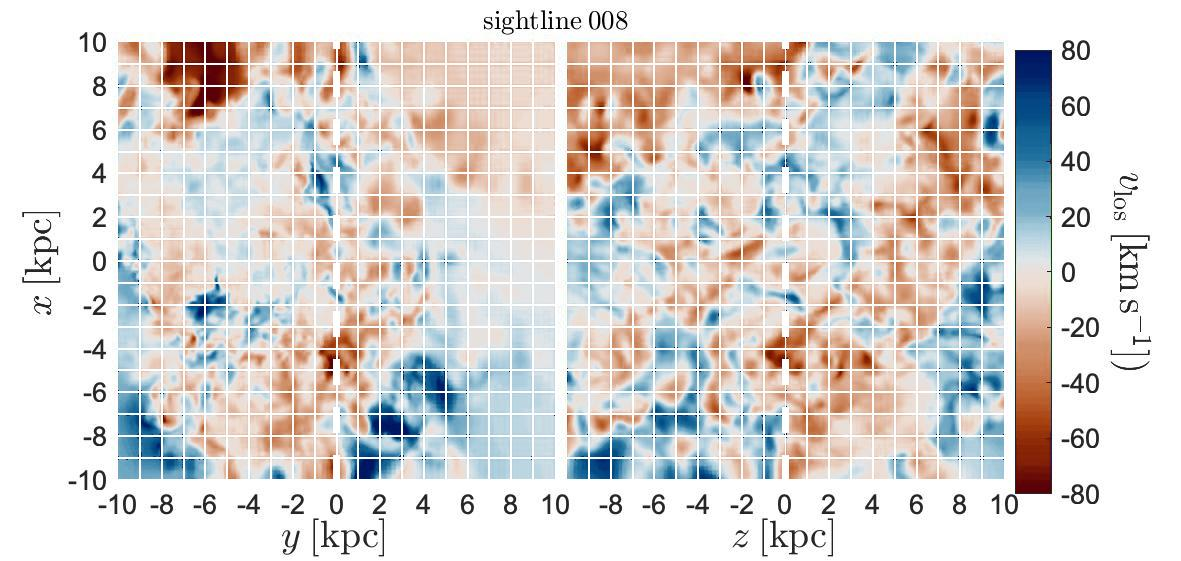
\includegraphics[width=0.49\textwidth]{figures/sample2/projections/velocity_projection_maps_SL_08.jpg}
    \caption{
    Density, temperature, metallicity, and line-of-sight velocity in a slice of the simulation used to generate \texttt{sample2}~\citep{mandelker2020Instability}.
    The dashed white line shows the location of one of the sightlines (sightline 08) forward-modeled to produce mock spectra.
    }
    \label{f: sample2 ray 08}
\end{figure*}

\begin{figure*}
    \centering
    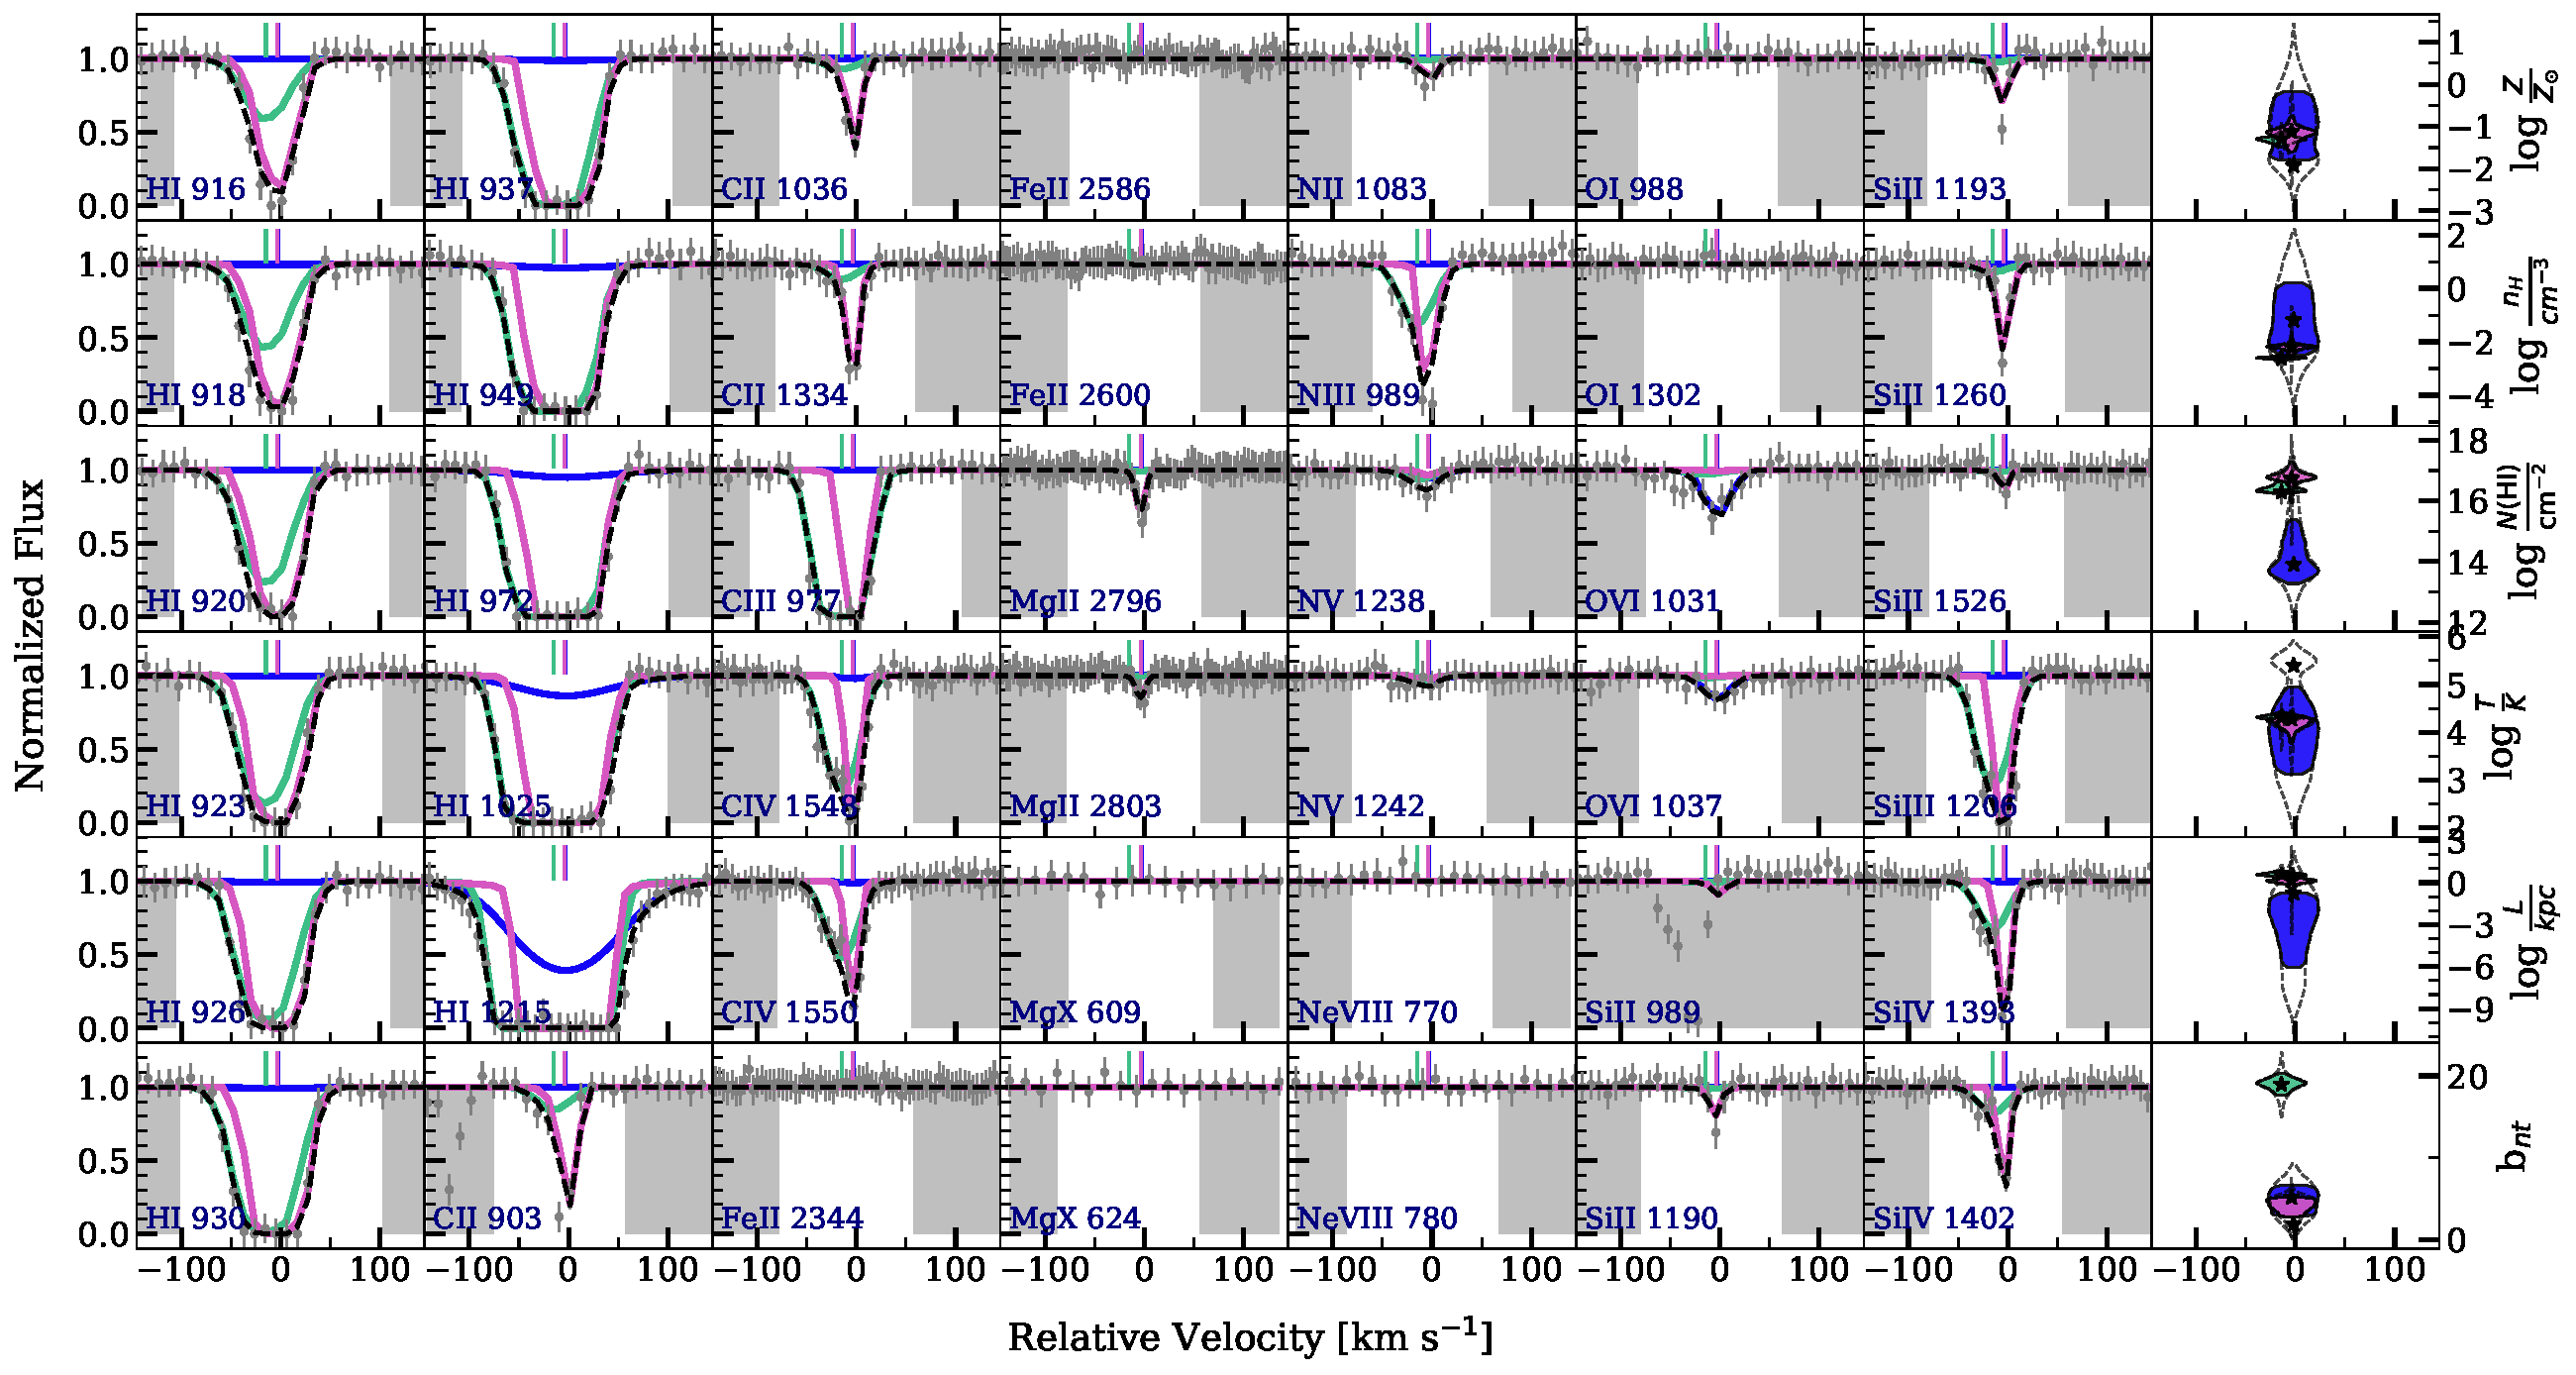
\includegraphics[width=\textwidth]{figures/sample2/best_fits/0008.pdf}
    \caption{
    Mock spectra for sightline 08,
    best fit absorption profiles found by observers,
    and the parameters of the best fits.
    }
    \label{f: sample2 spectrum 08}
\end{figure*}
\begin{figure*}
    \centering
    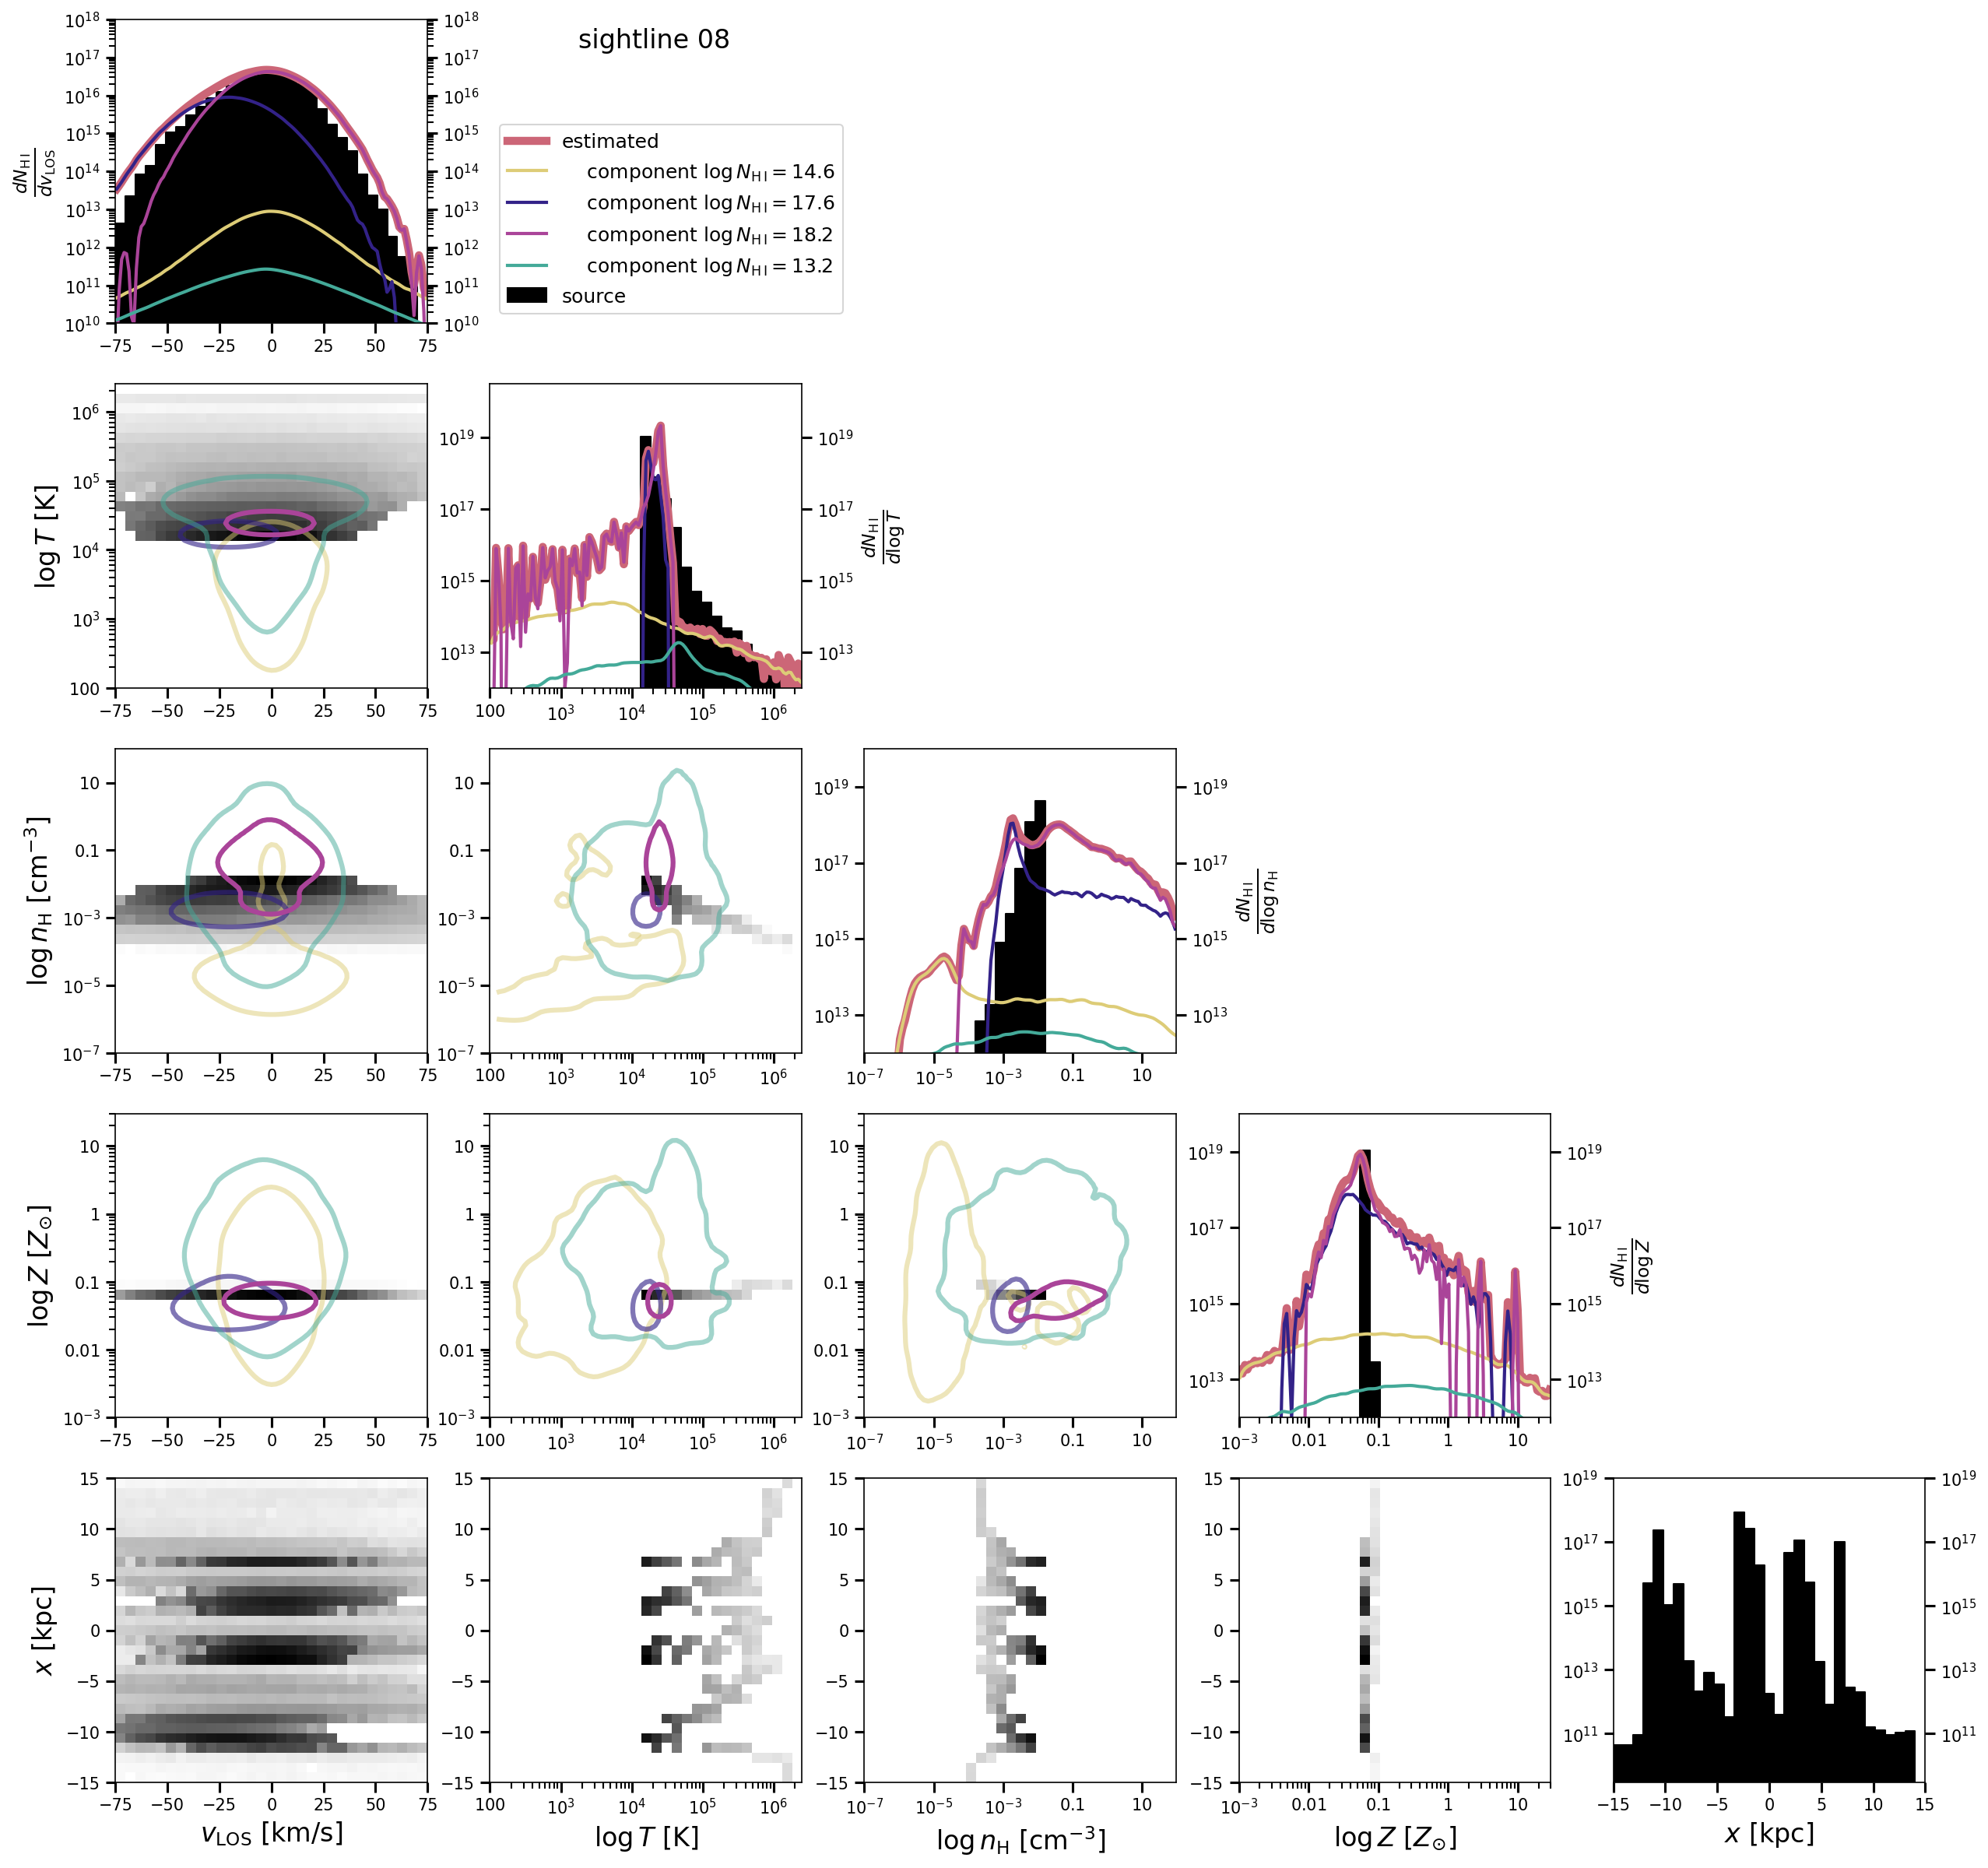
\includegraphics[height=0.45\textheight]{figures/sample2/original/sightline_0008.png}
    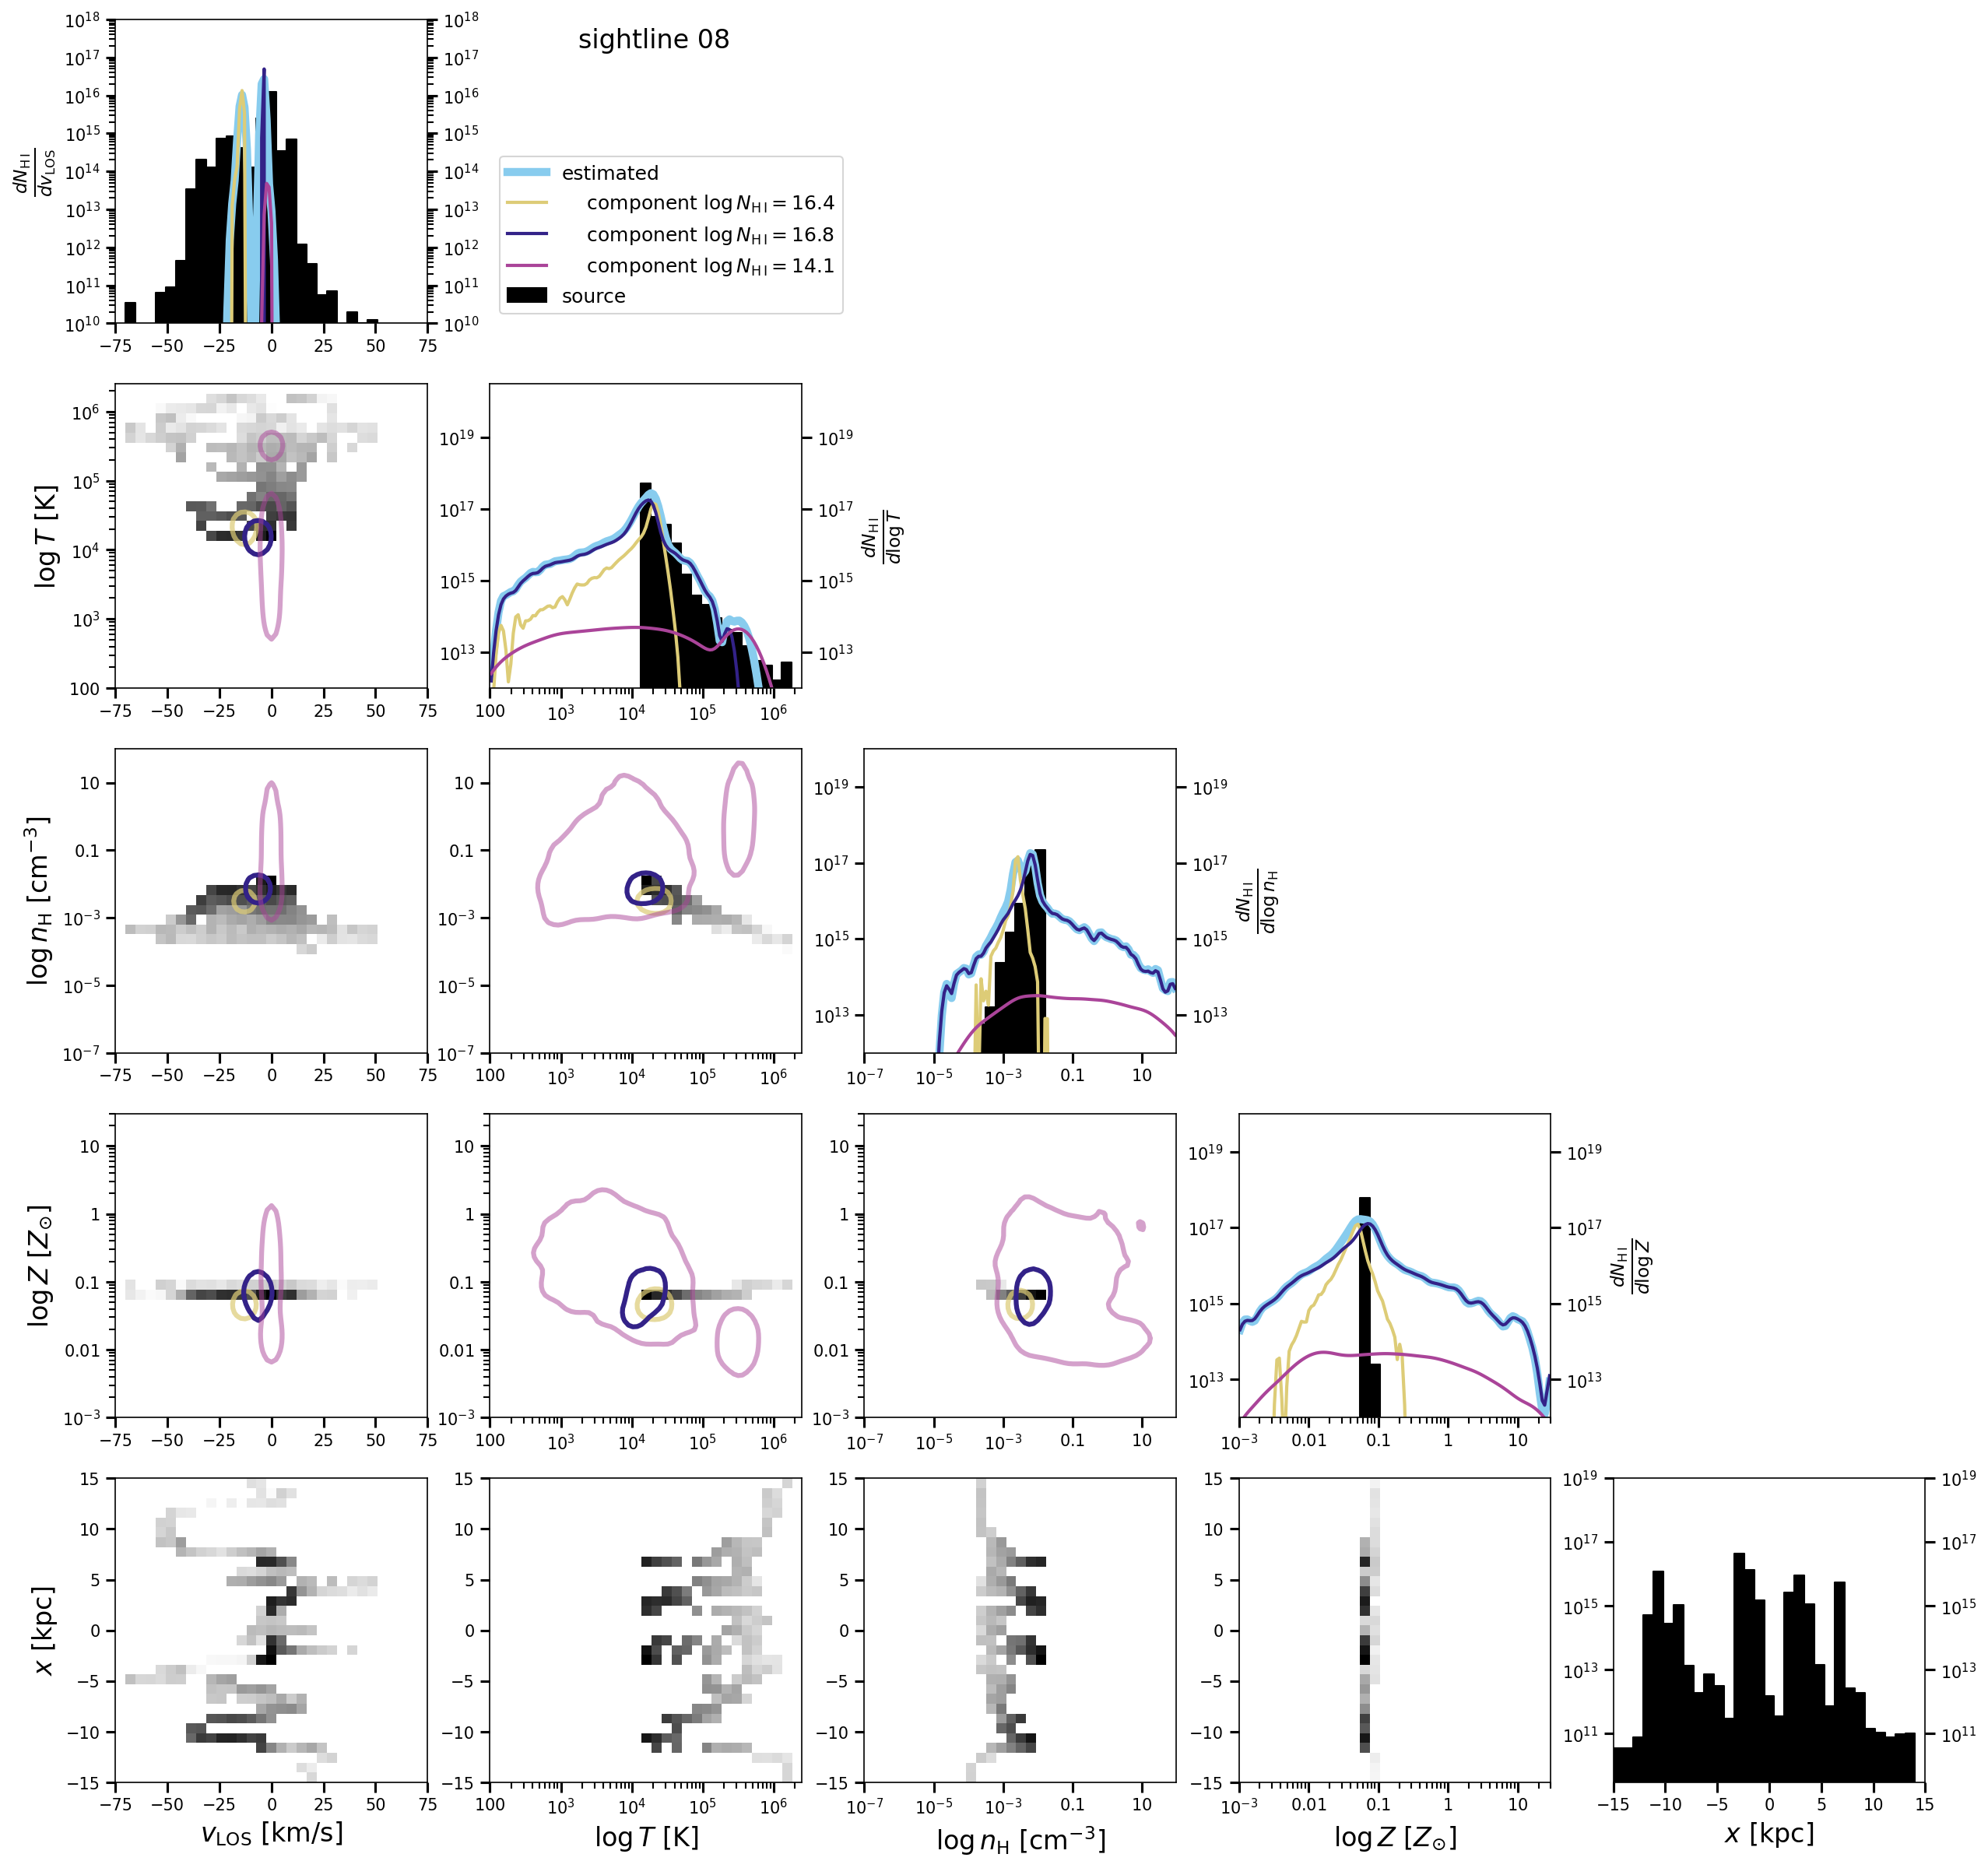
\includegraphics[height=0.45\textheight]{figures/sample2/high-z/sightline_0008.png}
    \label{f: sample2 08 corner}
    \caption{Same as Fig.~\ref{f: sample2 corner 03}, but for sightline 08.}
\end{figure*}

\begin{figure*}
    \centering
    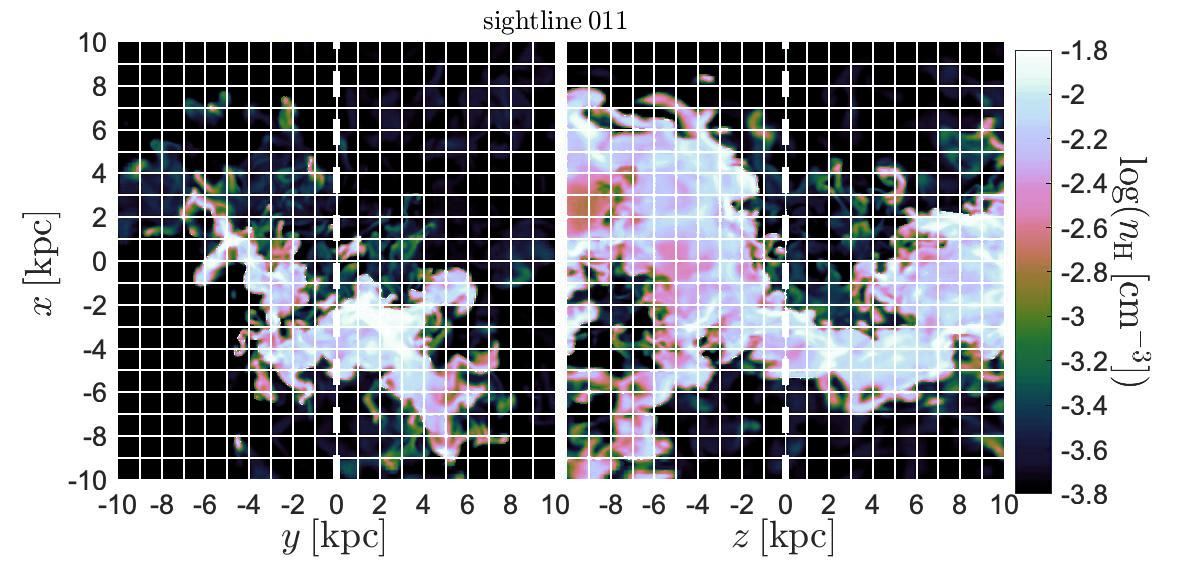
\includegraphics[width=0.49\textwidth]{figures/sample2/projections/density_projection_maps_SL_11.jpg}
    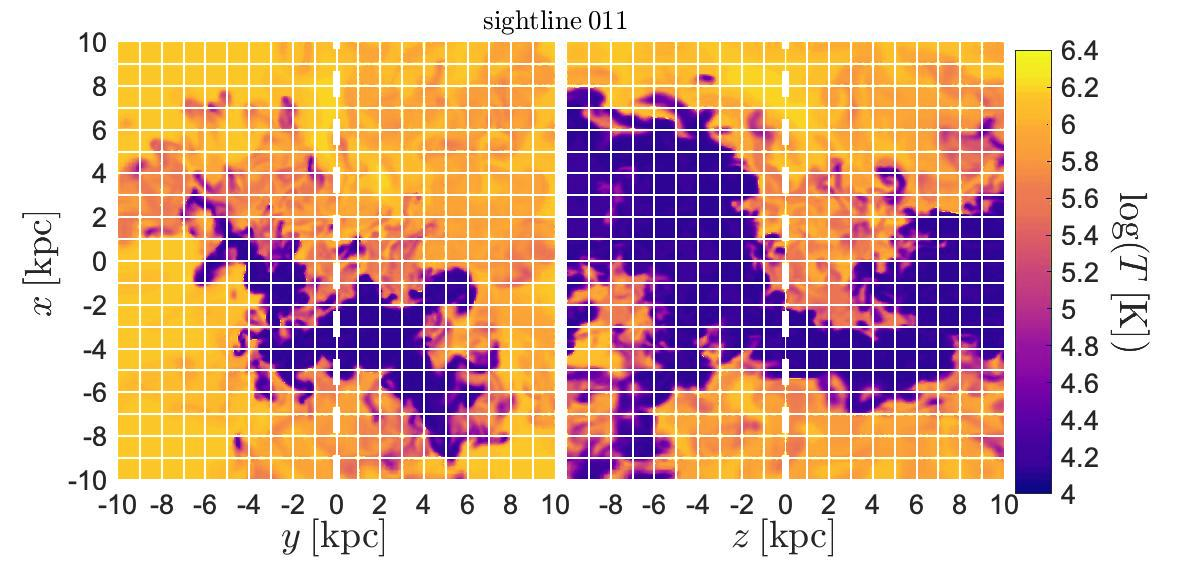
\includegraphics[width=0.49\textwidth]{figures/sample2/projections/temperature_projection_maps_SL_11.jpg} \\
    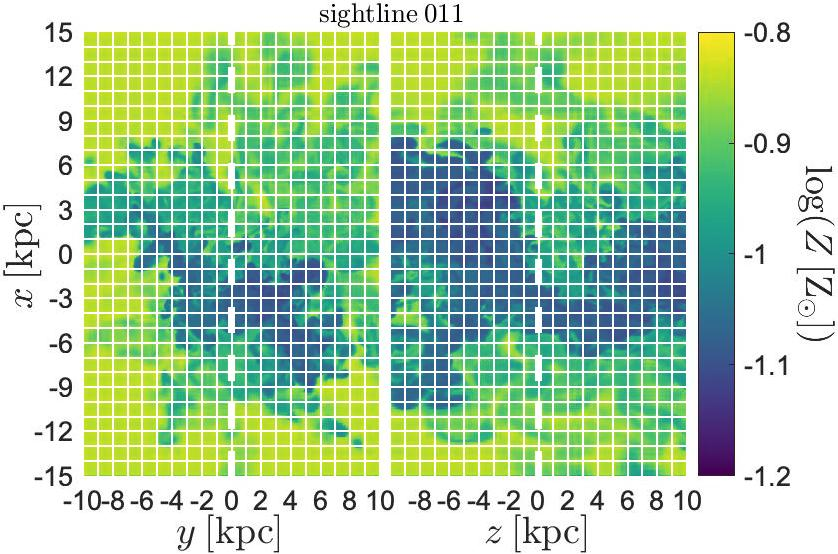
\includegraphics[width=0.49\textwidth]{figures/sample2/projections/metallicity_projection_maps_SL_11.jpg}
    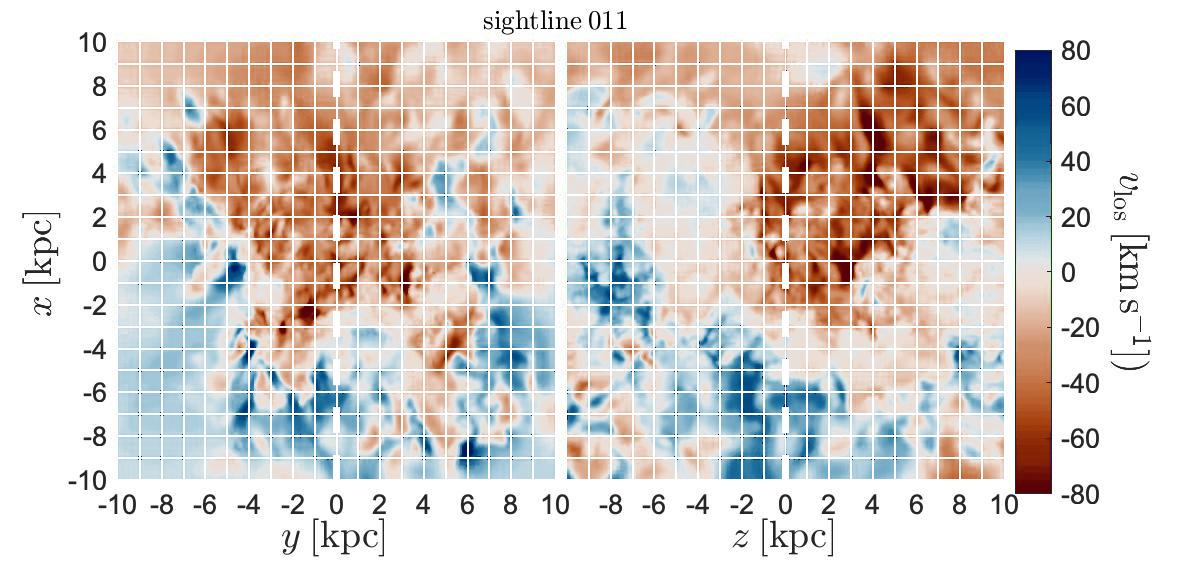
\includegraphics[width=0.49\textwidth]{figures/sample2/projections/velocity_projection_maps_SL_11.jpg}
    \caption{
    Density, temperature, metallicity, and line-of-sight velocity in a slice of the simulation used to generate \texttt{sample2}~\citep{mandelker2020Instability}.
    The dashed white line shows the location of one of the sightlines (sightline 11) forward-modeled to produce mock spectra.
    }
    \label{f: sample2 ray 11}
\end{figure*}

\begin{figure*}
    \centering
    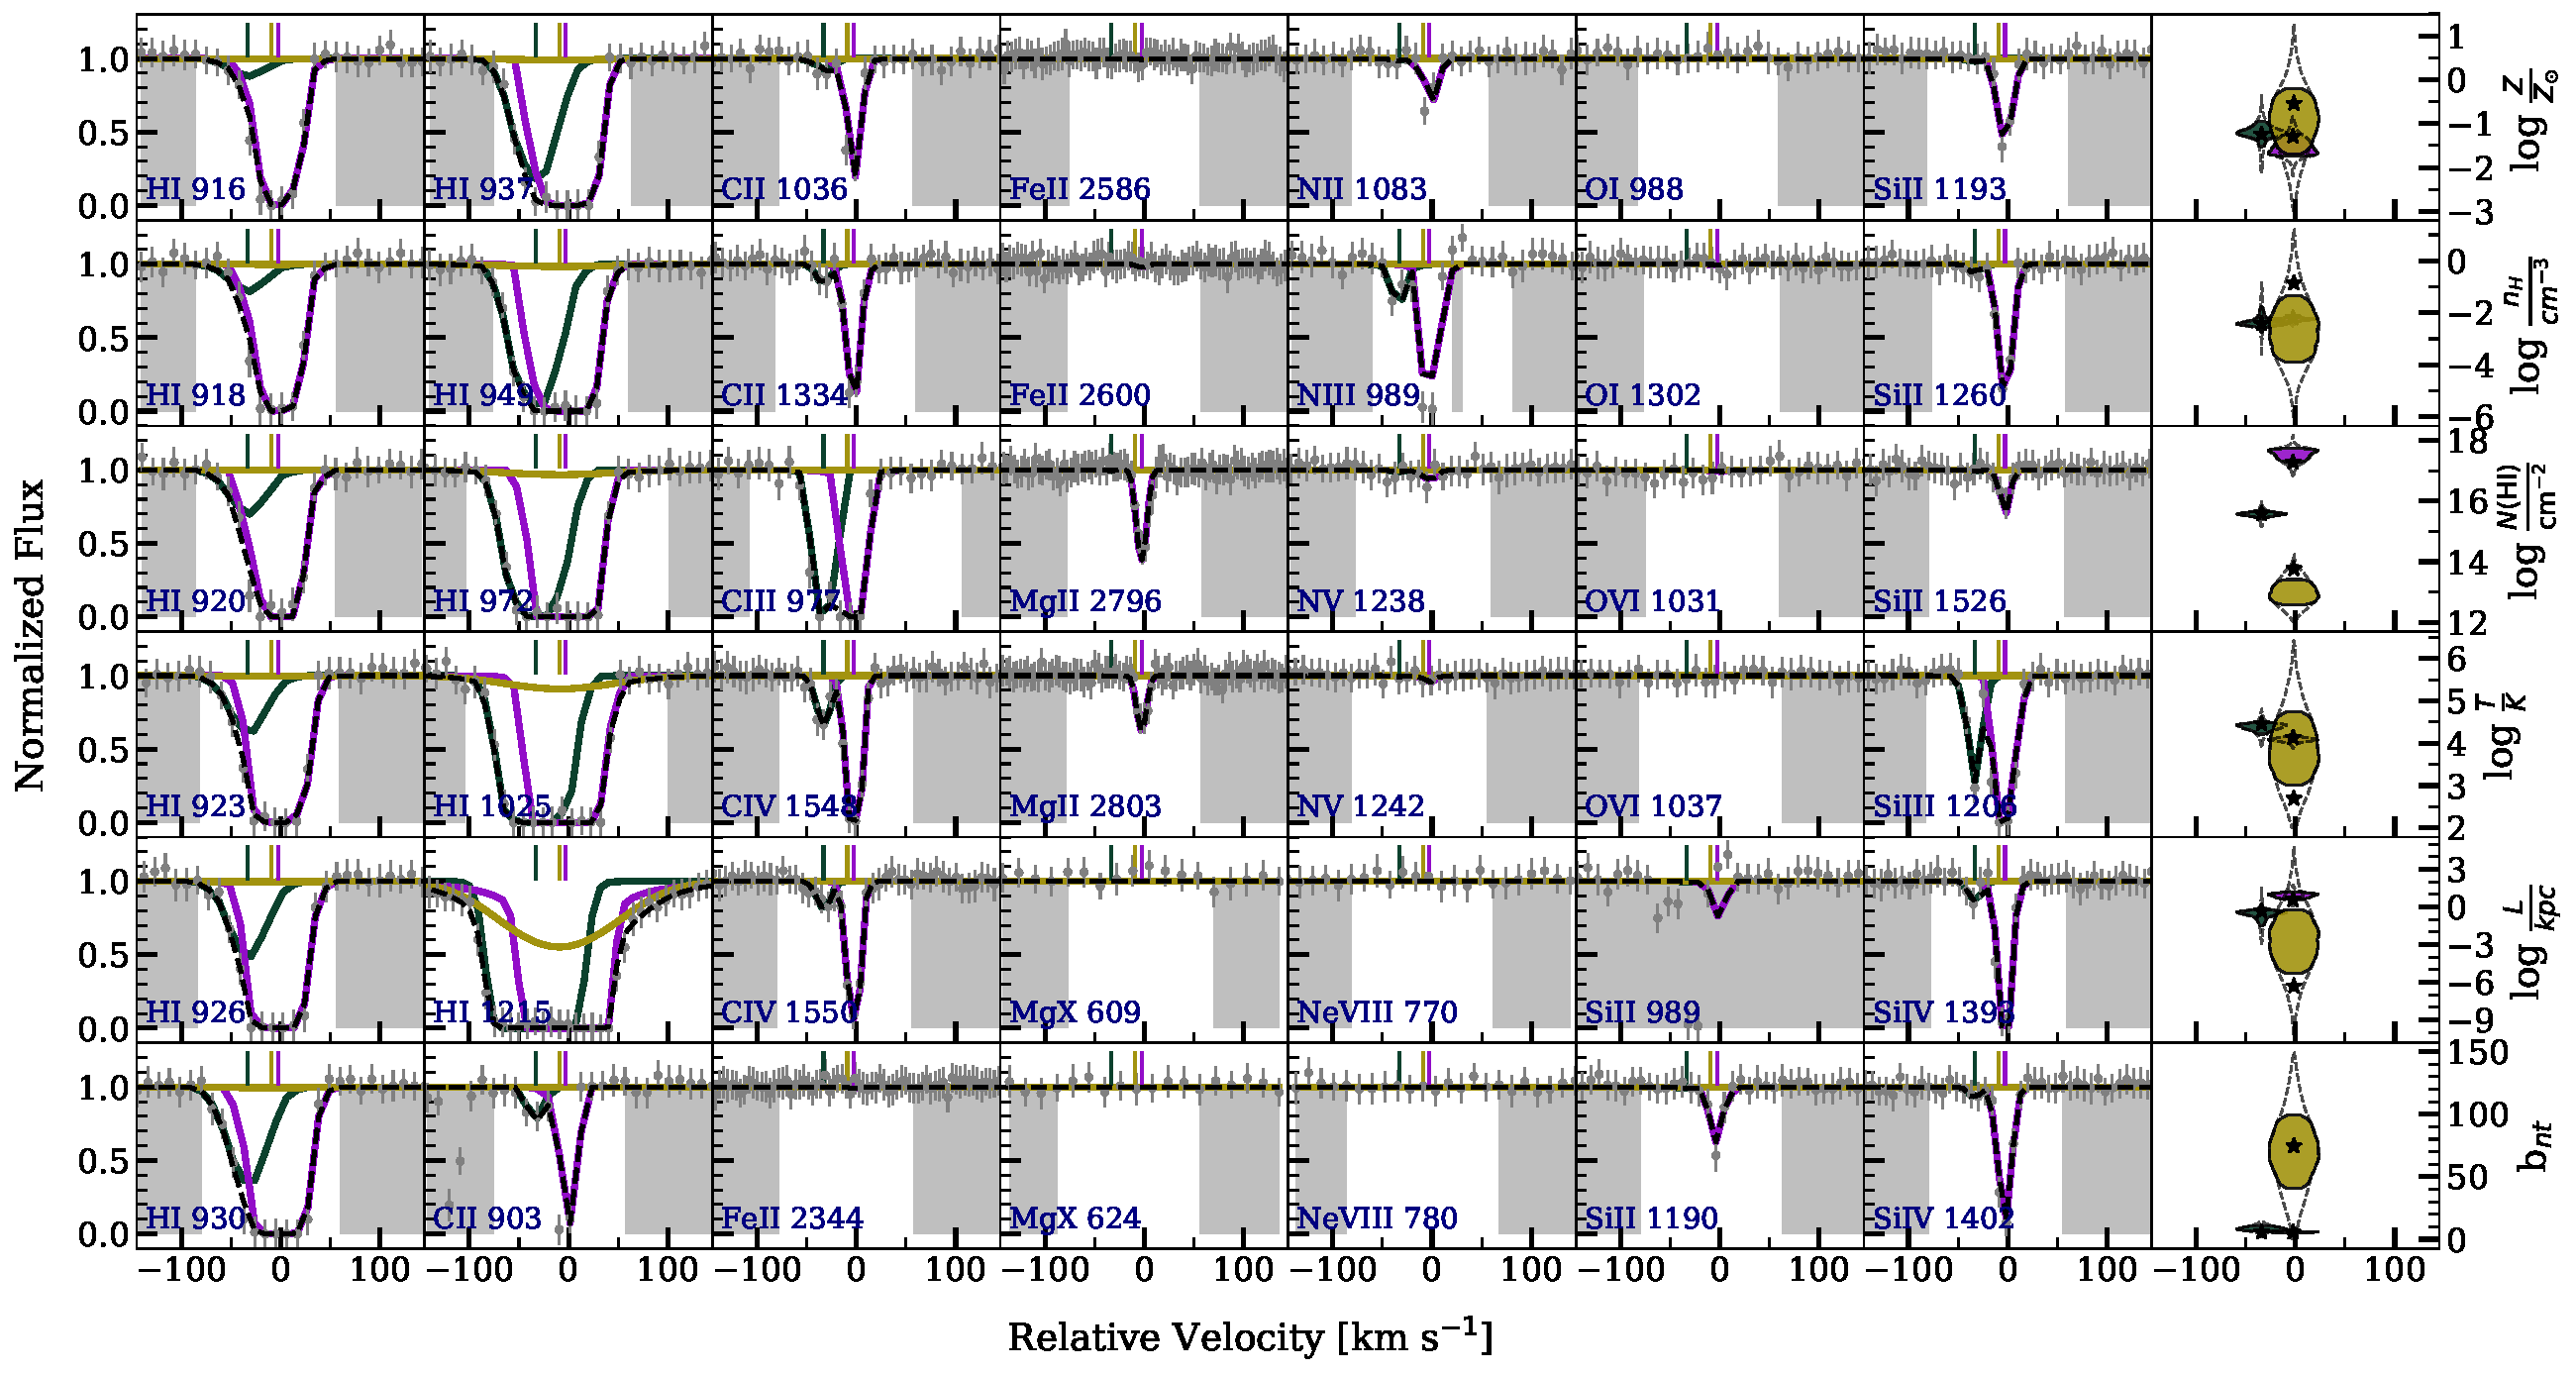
\includegraphics[width=\textwidth]{figures/sample2/best_fits/0011.pdf}
    \caption{
    Mock spectra for sightline 11,
    best fit absorption profiles found by observers,
    and the parameters of the best fits.
    }
    \label{f: sample2 spectrum 11}
\end{figure*}

\begin{figure*}
    \centering
    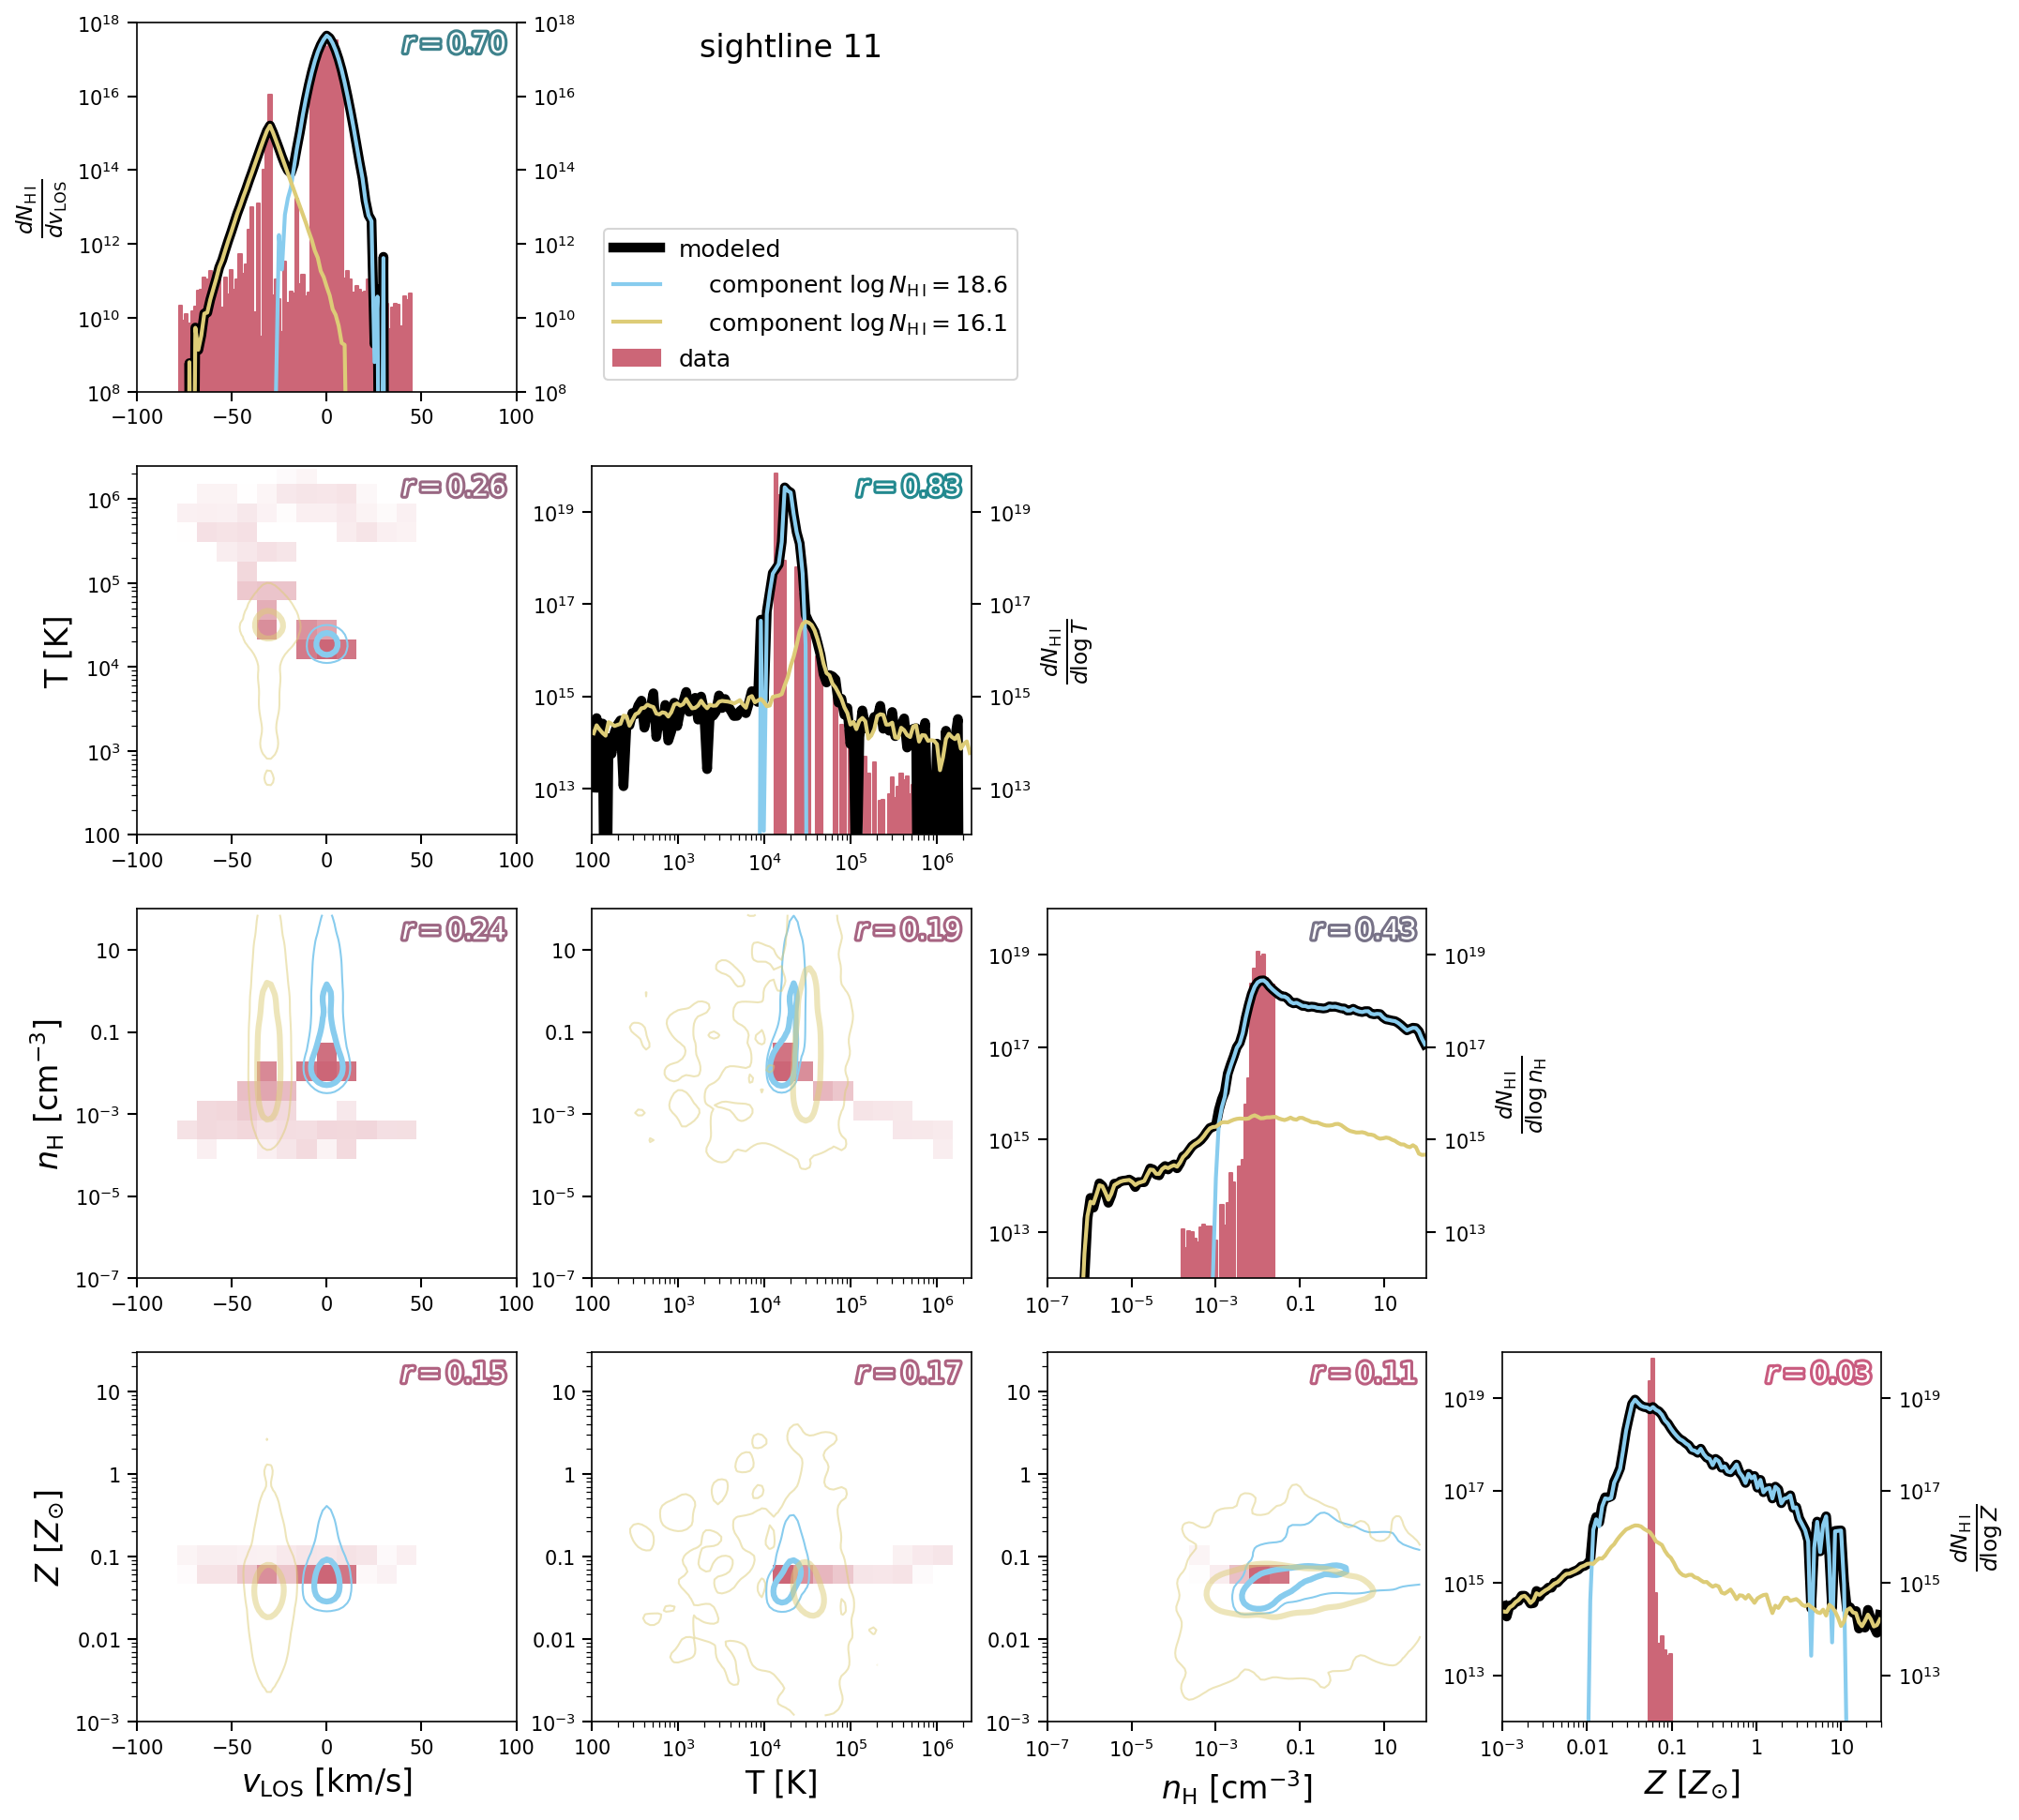
\includegraphics[height=0.45\textheight]{figures/sample2/original/sightline_0011.png}
    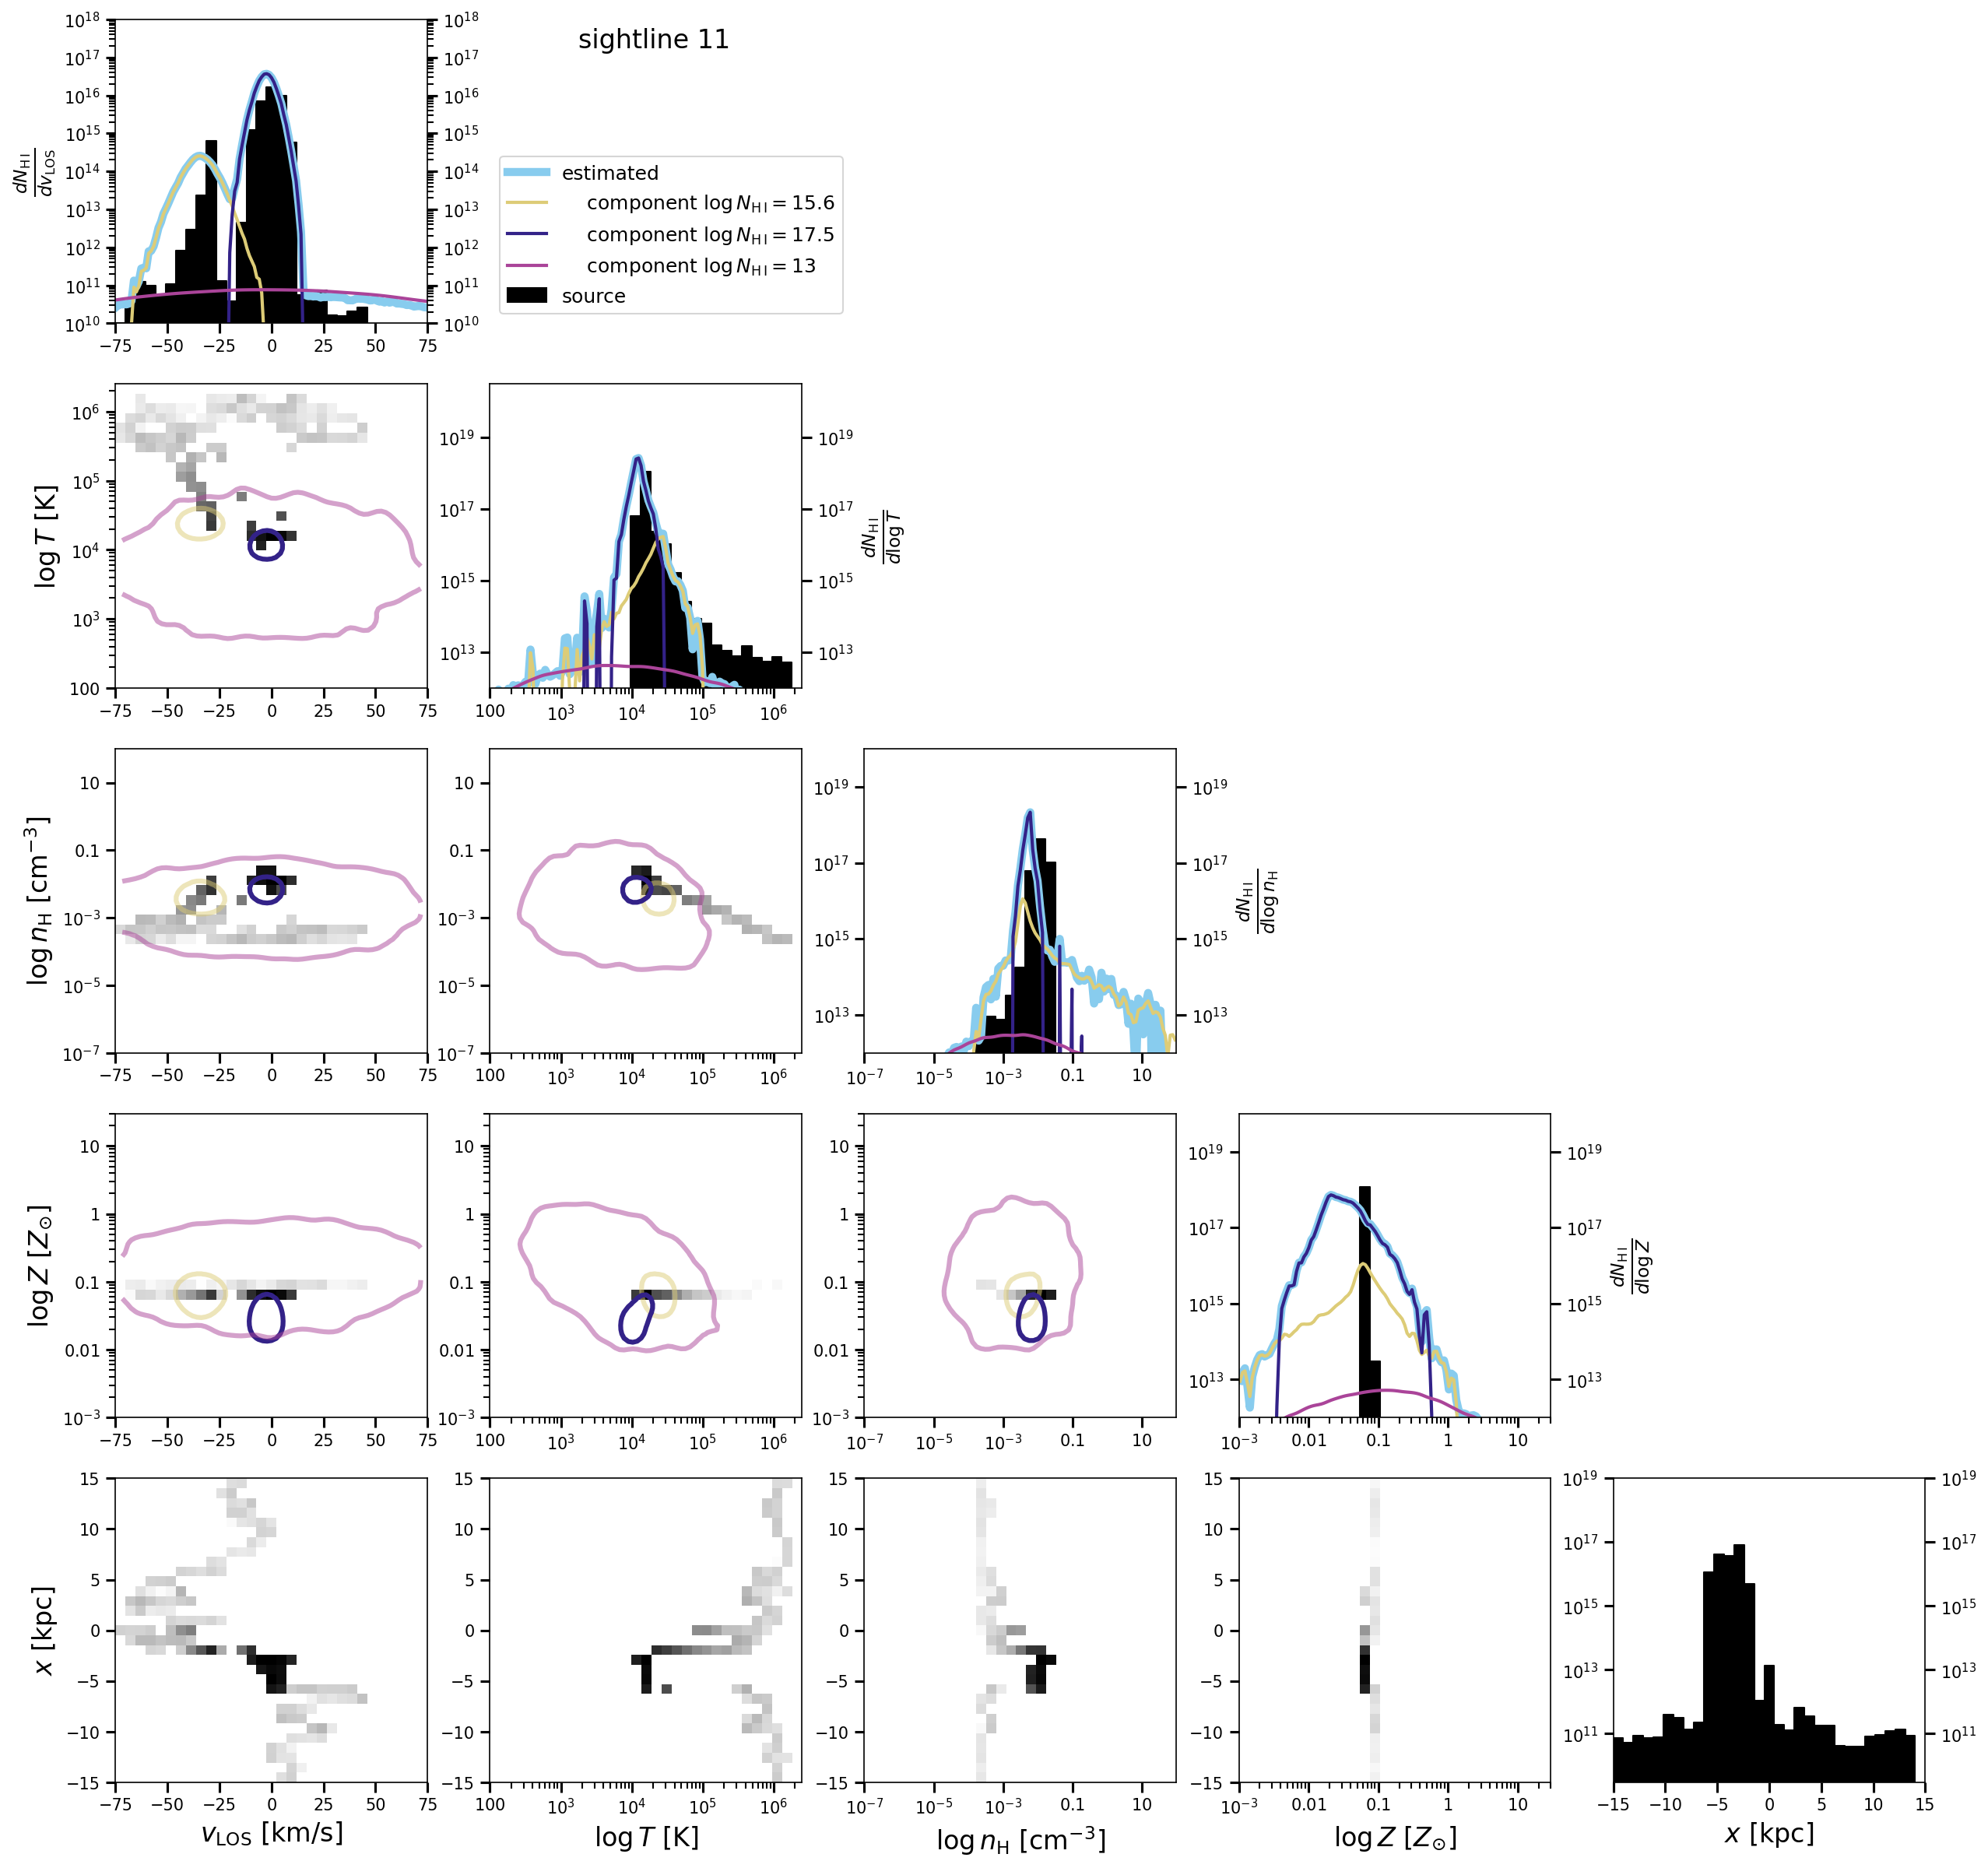
\includegraphics[height=0.45\textheight]{figures/sample2/high-z/sightline_0011.png}
    \label{f: sample2 11 corner}
    \caption{Same as Fig.~\ref{f: sample2 corner 03}, but for sightline 11.}
\end{figure*}

\begin{figure*}
    \centering
    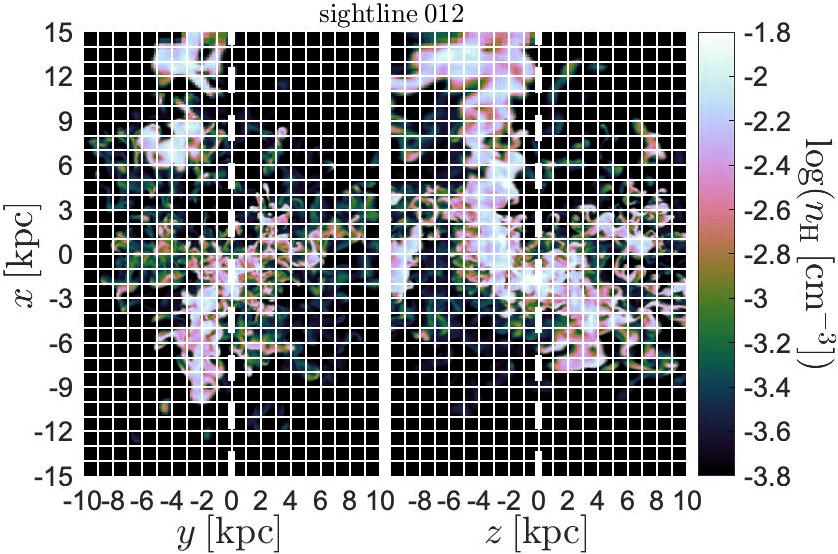
\includegraphics[width=0.49\textwidth]{figures/sample2/projections/density_projection_maps_SL_12.jpg}
    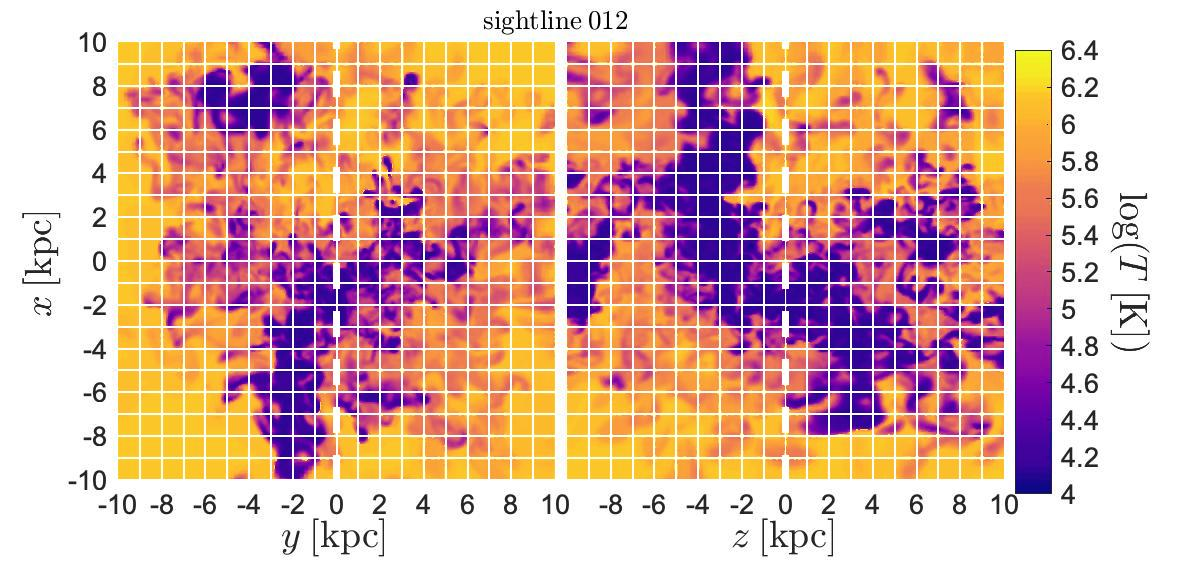
\includegraphics[width=0.49\textwidth]{figures/sample2/projections/temperature_projection_maps_SL_12.jpg} \\
    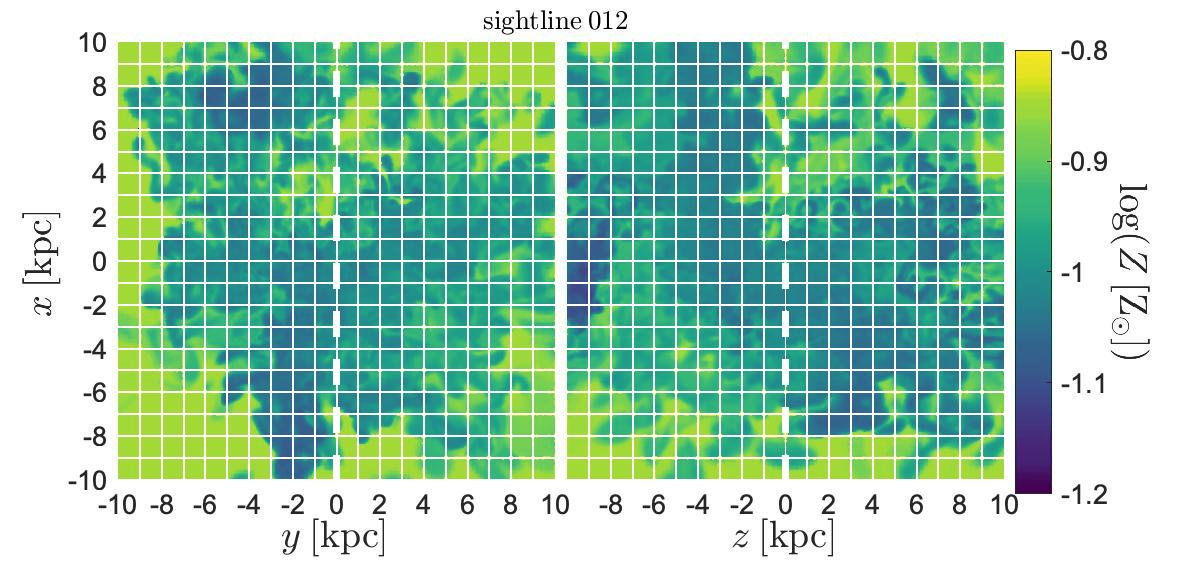
\includegraphics[width=0.49\textwidth]{figures/sample2/projections/metallicity_projection_maps_SL_12.jpg}
    \includegraphics[width=0.49\textwidth]{figures/sample2/projections/velocity_projection_maps_SL_12.jpg}
    \caption{
    Density, temperature, metallicity, and line-of-sight velocity in a slice of the simulation used to generate \texttt{sample2}~\citep{mandelker2020Instability}.
    The dashed white line shows the location of one of the sightlines (sightline 12) forward-modeled to produce mock spectra.
    }
    \label{f: sample2 ray 12}
\end{figure*}

\begin{figure*}
    \centering
    \includegraphics[width=\textwidth]{figures/sample2/best_fits/0012.pdf}
    \caption{
    Mock spectra for sightline 12,
    best fit absorption profiles found by observers,
    and the parameters of the best fits.
    }
    \label{f: sample2 spectrum 12}
\end{figure*}

\begin{figure*}
    \centering
    \includegraphics[height=0.45\textheight]{figures/sample2/original/sightline_0012.png}
    \includegraphics[height=0.45\textheight]{figures/sample2/high-z/sightline_0012.png}
    \label{f: sample2 12 corner}
    \caption{Same as Fig.~\ref{f: sample2 corner 03}, but for sightline 12.}
\end{figure*}

\begin{figure*}
    \centering
    \includegraphics[width=0.49\textwidth]{figures/sample2/projections/density_projection_maps_SL_14.jpg}
    \includegraphics[width=0.49\textwidth]{figures/sample2/projections/temperature_projection_maps_SL_14.jpg} \\
    \includegraphics[width=0.49\textwidth]{figures/sample2/projections/metallicity_projection_maps_SL_14.jpg}
    \includegraphics[width=0.49\textwidth]{figures/sample2/projections/velocity_projection_maps_SL_14.jpg}
    \caption{
    Density, temperature, metallicity, and line-of-sight velocity in a slice of the simulation used to generate \texttt{sample2}~\citep{mandelker2020Instability}.
    The dashed white line shows the location of one of the sightlines (sightline 14) forward-modeled to produce mock spectra.
    }
    \label{f: sample2 ray 14}
\end{figure*}

\begin{figure*}
    \centering
    \includegraphics[width=\textwidth]{figures/sample2/best_fits/0014.pdf}
    \caption{
    Mock spectra for sightline 14,
    best fit absorption profiles found by observers,
    and the parameters of the best fits.
    }
    \label{f: sample2 spectrum 14}
\end{figure*}

\begin{figure*}
    \centering
    \includegraphics[height=0.45\textheight]{figures/sample2/original/sightline_0014.png}
    \includegraphics[height=0.45\textheight]{figures/sample2/high-z/sightline_0014.png}
    \label{f: sample2 14 corner}
    \caption{Same as Fig.~\ref{f: sample2 corner 03}, but for sightline 14.}
\end{figure*}

\begin{figure*}
    \centering
    \includegraphics[width=0.49\textwidth]{figures/sample2/projections/density_projection_maps_SL_15.jpg}
    \includegraphics[width=0.49\textwidth]{figures/sample2/projections/temperature_projection_maps_SL_15.jpg} \\
    \includegraphics[width=0.49\textwidth]{figures/sample2/projections/metallicity_projection_maps_SL_15.jpg}
    \includegraphics[width=0.49\textwidth]{figures/sample2/projections/velocity_projection_maps_SL_15.jpg}
    \caption{
    Density, temperature, metallicity, and line-of-sight velocity in a slice of the simulation used to generate \texttt{sample2}~\citep{mandelker2020Instability}.
    The dashed white line shows the location of one of the sightlines (sightline 15) forward-modeled to produce mock spectra.
    }
    \label{f: sample2 ray 15 appendix}
\end{figure*}

\begin{figure*}
    \centering
    \includegraphics[width=\textwidth]{figures/sample2/best_fits/0015.pdf}
    \caption{
    Mock spectra for sightline 15,
    best fit absorption profiles found by observers,
    and the parameters of the best fits.
    }
    \label{f: sample2 spectrum 15 appendix}
\end{figure*}

\begin{figure*}
    \centering
    \includegraphics[height=0.45\textheight]{figures/sample2/original/sightline_0015.png}
    \includegraphics[height=0.45\textheight]{figures/sample2/high-z/sightline_0015.png}
    \label{f: sample2 15 corner}
    \caption{Same as Fig.~\ref{f: sample2 corner 03}, but for sightline 15.}
\end{figure*}

\begin{figure*}
    \centering
    \includegraphics[width=0.49\textwidth]{figures/sample2/projections/density_projection_maps_SL_16.jpg}
    \includegraphics[width=0.49\textwidth]{figures/sample2/projections/temperature_projection_maps_SL_16.jpg} \\
    \includegraphics[width=0.49\textwidth]{figures/sample2/projections/metallicity_projection_maps_SL_16.jpg}
    \includegraphics[width=0.49\textwidth]{figures/sample2/projections/velocity_projection_maps_SL_16.jpg}
    \caption{
    Density, temperature, metallicity, and line-of-sight velocity in a slice of the simulation used to generate \texttt{sample2}~\citep{mandelker2020Instability}.
    The dashed white line shows the location of one of the sightlines (sightline 16) forward-modeled to produce mock spectra.
    }
    \label{f: sample2 ray 16}
\end{figure*}

\begin{figure*}
    \centering
    \includegraphics[width=\textwidth]{figures/sample2/best_fits/0016.pdf}
    \caption{
    Mock spectra for sightline 16,
    best fit absorption profiles found by observers,
    and the parameters of the best fits.
    }
    \label{f: sample2 spectrum 16}
\end{figure*}

\begin{figure*}
    \centering
    \includegraphics[height=0.45\textheight]{figures/sample2/original/sightline_0016.png}
    \includegraphics[height=0.45\textheight]{figures/sample2/high-z/sightline_0016.png}
    \label{f: sample2 16 corner}
    \caption{Same as Fig.~\ref{f: sample2 corner 03}, but for sightline 16.}
\end{figure*}

\begin{figure*}
    \centering
    \includegraphics[width=0.49\textwidth]{figures/sample2/projections/density_projection_maps_SL_19.jpg}
    \includegraphics[width=0.49\textwidth]{figures/sample2/projections/temperature_projection_maps_SL_19.jpg} \\
    \includegraphics[width=0.49\textwidth]{figures/sample2/projections/metallicity_projection_maps_SL_19.jpg}
    \includegraphics[width=0.49\textwidth]{figures/sample2/projections/velocity_projection_maps_SL_19.jpg}
    \caption{
    Density, temperature, metallicity, and line-of-sight velocity in a slice of the simulation used to generate \texttt{sample2}~\citep{mandelker2020Instability}.
    The dashed white line shows the location of one of the sightlines (sightline 19) forward-modeled to produce mock spectra.
    }
    \label{f: sample2 ray 19}
\end{figure*}

\begin{figure*}
    \centering
    \includegraphics[width=\textwidth]{figures/sample2/best_fits/0019.pdf}
    \caption{
    Mock spectra for sightline 19,
    best fit absorption profiles found by observers,
    and the parameters of the best fits.
    }
    \label{f: sample2 spectrum 19}
\end{figure*}

\begin{figure*}
    \centering
    \includegraphics[height=0.45\textheight]{figures/sample2/original/sightline_0019.png}
    \includegraphics[height=0.45\textheight]{figures/sample2/high-z/sightline_0019.png}
    \label{f: sample2 19 corner}
    \caption{Same as Fig.~\ref{f: sample2 corner 03}, but for sightline 19.}
\end{figure*}

This section includes additional figures for sample2.

%%%%%%%%%%%%%%%%%%%%%%%%%%%%%%%%%%%%%%%%%%%%%%%%%%


% Don't change these lines
\bsp	% typesetting comment
\label{lastpage}
\end{document}

% End of mnras_template.tex
